\section{Double Multilayer Monochromator (DMM)}
\vspace*{-\baselineskip}
\begin{center}
\begin{table} [ht]
\small
\begin{tabular}[bhp]{|p{0.4\textwidth} | p{0.5\textwidth}|}
\hline
Deflection & Vertical \\
Distance from source (1st ML) & 15.165 m \\
Beamline aperture & 1.8 mrad × 0.4 mrad (Hor. × Ver.) \\
Beam size @ 1st mirror & 29 mm × 6 mm (Hor. × Ver.) \\
Working energy & 8 – 50 [keV] \\
ML length & 500 mm \\
Distance between MLs & 510 mm \\
Offset (variable) & Min. 4.2 – Max. 16.0 [mm] \\
Theta (Bragg angle) & -0.5 to +2.5 [deg] \\
Bragg resolution & 0.5 µrad \\
Input beam power on 1st mirror & 133 W \\
% Supplier & CINEL Strumenti Scientifici S.r.l. \\
\hline
\end{tabular}
\label{tab:DMM_general}
\end{table}
\end{center}

\setlength{\belowcaptionskip}{-15pt}
\vspace*{-\baselineskip}

\begin{figure} [!ht]
\centering
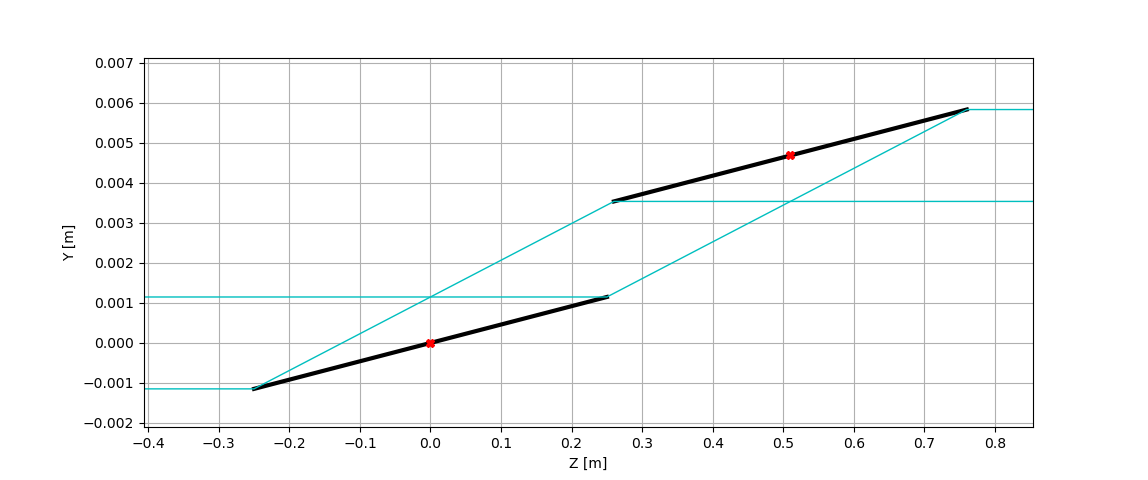
\includegraphics[width=0.9\textwidth]{./../figures/operation/DMM_mirrors_d3_E45_gr0.263_offset4.68.png}
\caption{\label{fig:DMM_mirrors_45keV} d-spacing: 3 nm; E: 45 keV; Grazing: 0.263 deg; offset: 4.68 mm.}
\end{figure}

\setlength{\belowcaptionskip}{-8pt}
\vspace*{-\baselineskip}

\begin{figure} [!ht]
\centering
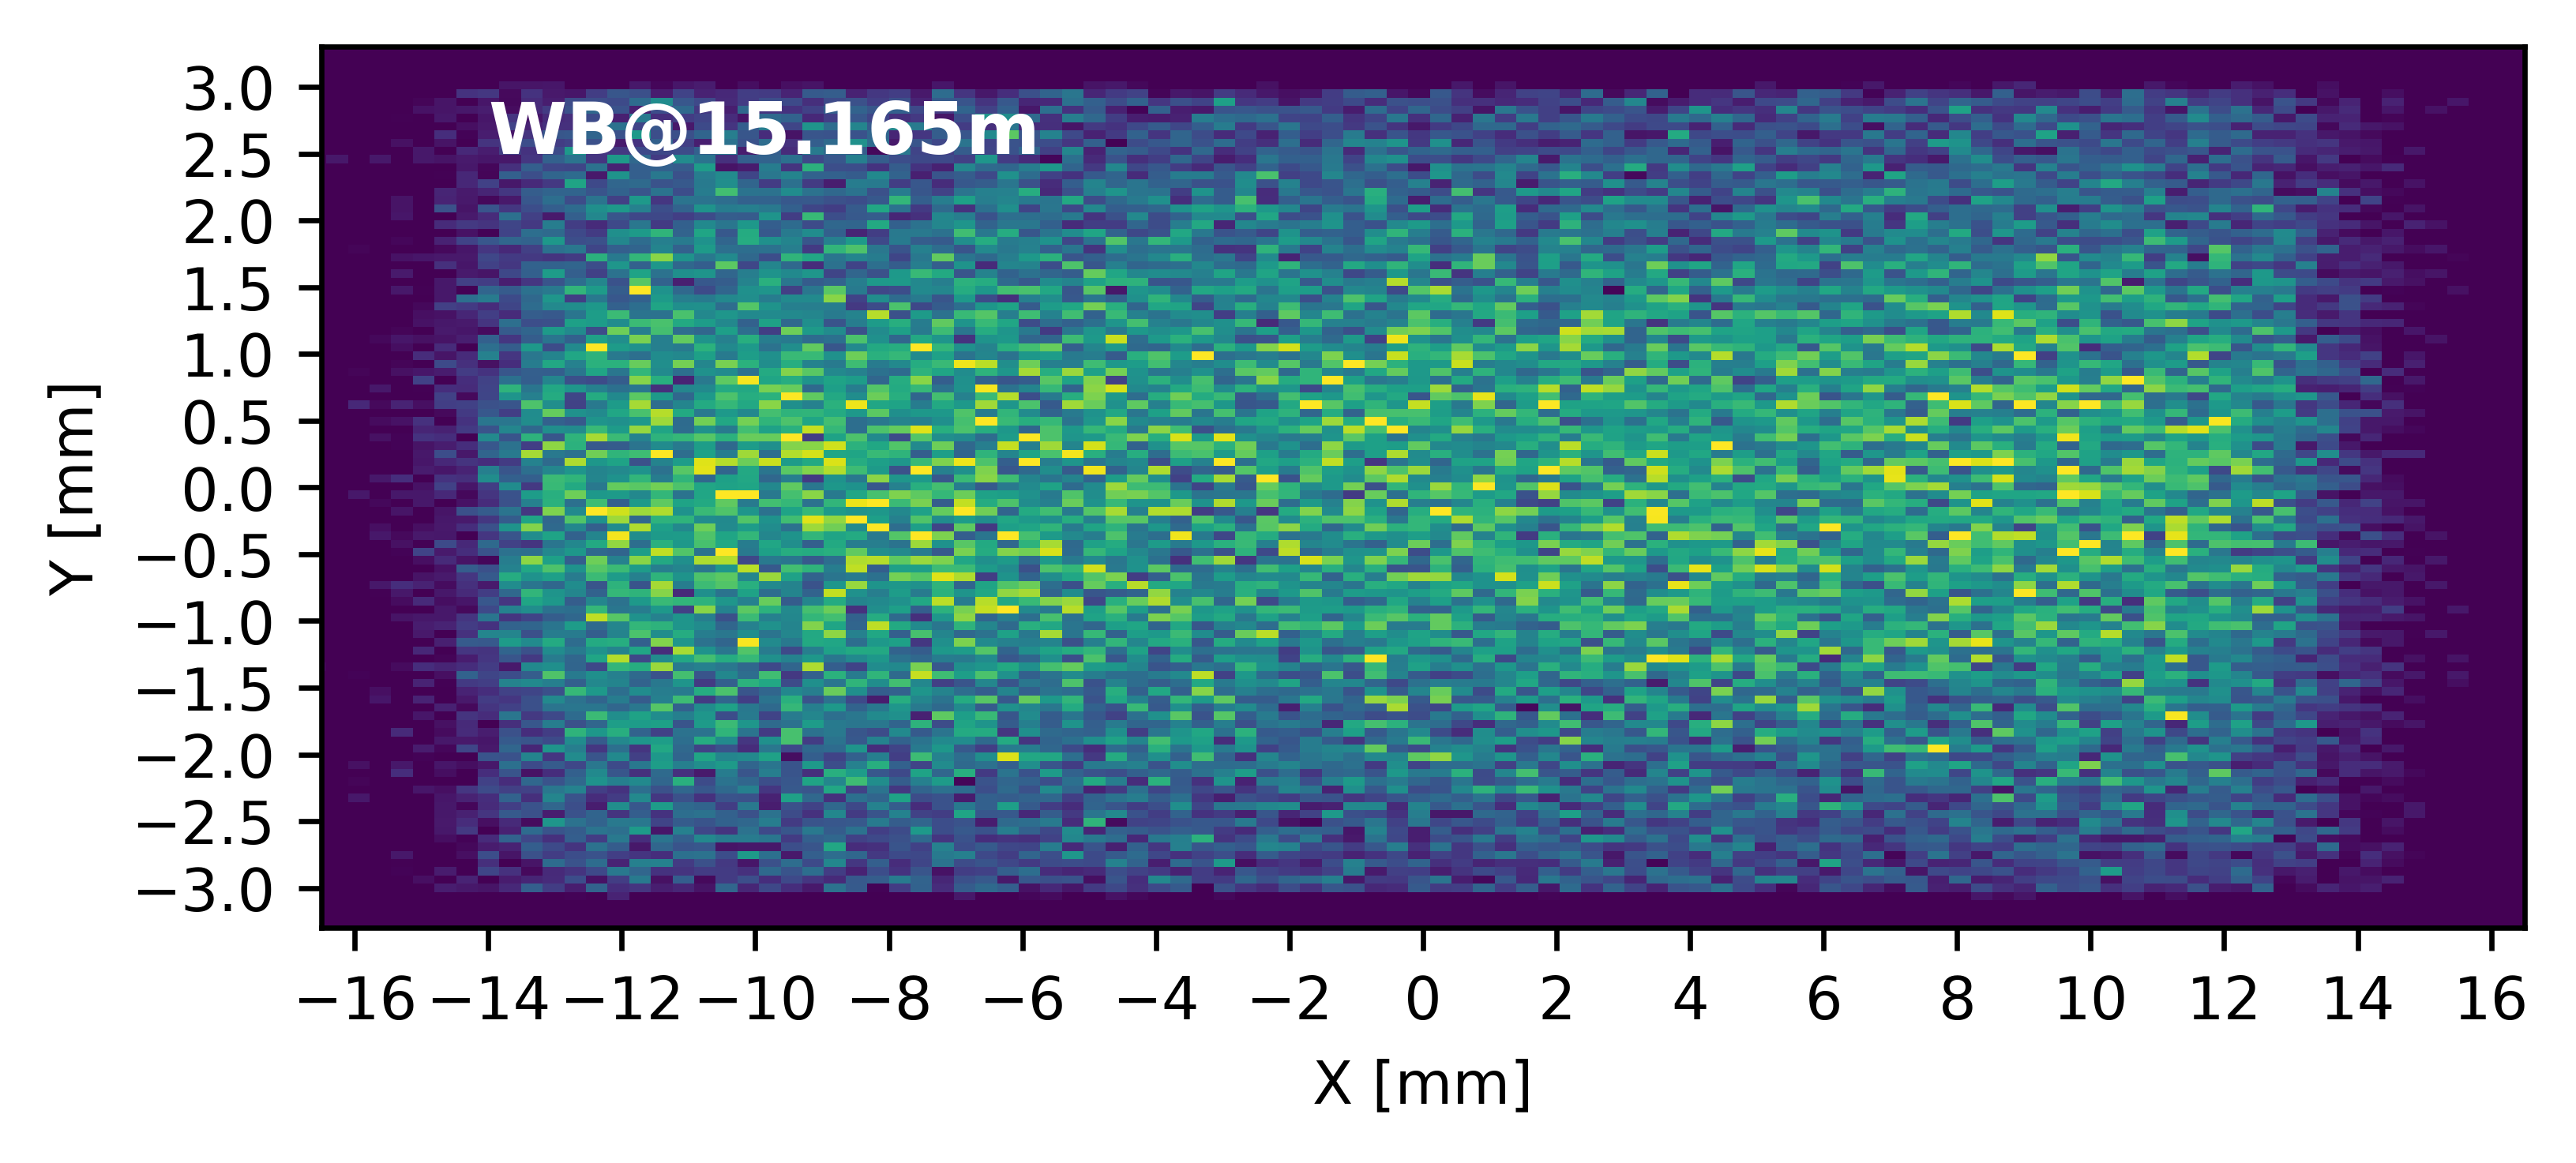
\includegraphics[width=0.8\textwidth]{./../../beam_snapshots/WB_snapshot_15.165.png}
\caption{\label{fig:snapshot_ML1} White beam (5-60 keV) snapshot at 15.165 m from source (center position of ML1).}
\end{figure}
\setlength{\belowcaptionskip}{-15pt}

%%%%%%%%%%%%%%%%%%%%%%%%%%%%%%%%%%%%%%%%%%%%%%%%%%%%%%%%%%%%%%%%%%%%%%%%%%%%%%%%%%%%
\clearpage
\subsection{Substrates}
The ML length was increased to 500 mm. A drawing of the proposed substrate size is attached. The substrate size and optical quality (tentative) are reported in Table \ref{tab:substrates}.

\begin{center}
\begin{table} [ht]
\begin{tabular}[bhp]{|p{0.4\textwidth} | p{0.5\textwidth}|}
\hline
Substrate dimension & 500 mm × 70 mm × 60 mm \\
 & (see drawing attached) \\
\hline
Coated area & 500 mm × 25 mm (2 stripes) \\
\hline
Surface roughness & $< 0.3$ nm rms \\
\hline
Slope error along Z & $\leq 0.3$ $\mu rad$ rms \\
(beam direction) & \\
\hline
Slope error along X & $< 20$ $\mu rad$ rms \\
(perpendicular to the beam) & \\
\hline
\end{tabular}
\caption{\label{tab:substrates} BEATS DMM substrates.}
\end{table}
\end{center}

%%%%%%%%%%%%%%%%%%%%%%%%%%%%%%%%%%%%%%%%%%%%%%%%%%%%%%%%%%%%%%%%%%%%%%%%%%%%%%%%%%%%
\subsection{ML coatings}
\textbf{Following the increase in ML length to 500 mm the d-spacing of the high-energy stripe is changed back from 2.5 nm to 3.0 nm.} This gives approx. +50\% int. reflectivity (dE/E increases from 2.3\% to 3.2\%). Thanks to the increased mirror length, the useful vertical part of the beam is intercepted even at minimum grazing and even with a d-spacing of 3.0 nm. Coating specs of the two ML stripes are given in Table \ref{tab:coatings}.
\begin{center}
\begin{table}[h]
\begin{tabular}[bhp]{| l | c | c |}
\hline
 & \textbf{STRIPE 1} & \textbf{STRIPE 2} \\
 & \textbf{$[W/B_{4}C]_{100} - d 3.0 nm $} & \textbf{$[Ru/B_{4}C]_{65} - d 4.0 nm $} \\
\hline
Materials & W/B4C & Ru/B4C \\
d-spacing [nm] & 3.0 & 4.0 \\
d-spacing gradient along Z (O.A. 500 mm) & \multicolumn{2}{c|}{3.297 \% (0.00659 \% / mm)} \\ 
N. bilayers & 100 & 65 \\
Duty cycle $\gamma$ & 0.5 & 0.5 \\
Energies [keV] & 20 – 50 & 8 - 22 \\
dE/E & ~ 3.2 \% & ~ 3.1 \% \\
Coated area & \multicolumn{2}{c|}{480 (500) mm × 25 mm} \\
Theta (Bragg angle) [deg] & 0.23 – 0.59 & 0.41 - 1.00 \\
\hline
\end{tabular}
\caption{\label{tab:coatings} BEATS multilayer coatings.}
\end{table}
\end{center}

%%%%%%%%%%%%%%%%%%%%%%%%%%%%%%%%%%%%%%%%%%%%%%%%%%%%%%%%%%%%%%%%%%%%%%%%%%%%%%%%%%%%
\clearpage
\subsection{Raytracing}
\begin{wrapfigure}{r}{0.3\linewidth}
\centering
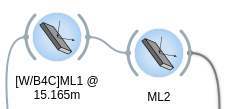
\includegraphics[width=0.3\textwidth]{images/DMM_oasys.png}
\caption{\label{fig:DMM_oasys} Double Multilayer Monochromator in Oasys Shadow.}
\end{wrapfigure}

The double-bounce DMM is modelled with two Shadow Plane Mirror widgets in series (Figure \ref{fig:DMM_oasys}). ML reflectivity is modelled with a Shadow PreMLayer widget as shown in Figure \ref{fig:PreMLayer}. The mirror surface is modified with Surface Error external splines with varying longitudinal slope error (0.1, 0.2, 0.3, 0.4 and 0.5 $\mu rad$ RMS). These modified surfaces (\ref{fig:fractals}) are simulated with the Shadow PreProcessor - Height Profile Simulator widget. The transversal slope error is kept constant at 20 $\mu rad$ RMS and fractal profiles are chosen. 

\begin{figure}  % spans both columns
\begin{subfigure}{0.5\textwidth}
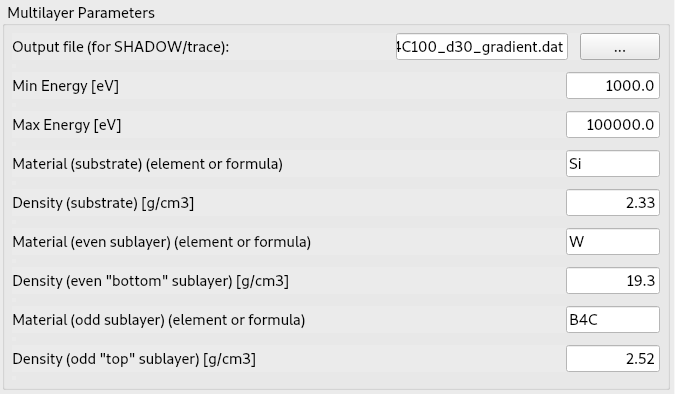
\includegraphics[width=\linewidth]{images/MLspecs_a.png}
\end{subfigure}
\hfill % maximize the horizontal distance between the graphs
\begin{subfigure}{0.5\textwidth}
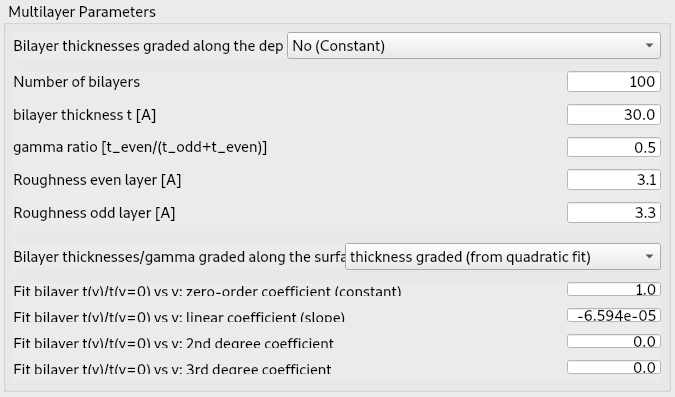
\includegraphics[width=\linewidth]{images/MLspecs_b.png}
\end{subfigure}
\caption{\label{fig:PreMLayer} PreMLayer widget settings in Shadow. }
\end{figure}

\begin{figure}[!htb]
\minipage{0.32\textwidth}
  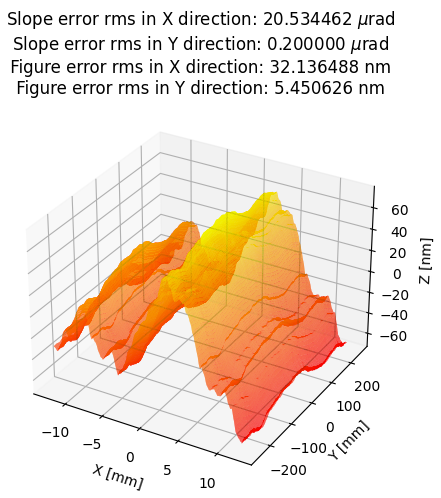
\includegraphics[width=\linewidth]{./../figures/slope_error/surface_error_profile_500x25_02x20urad.png}
  % \caption{A really Awesome Image}\label{fig:awesome_image1}
\endminipage\hfill
\minipage{0.32\textwidth}
  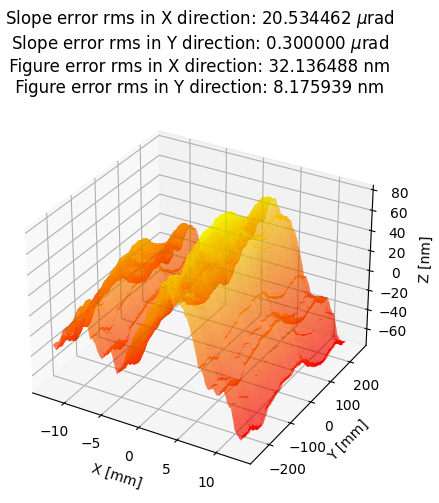
\includegraphics[width=\linewidth]{./../figures/slope_error/surface_error_profile_500x25_03x20urad.png}
  % \caption{A really Awesome Image}\label{fig:awesome_image2}
\endminipage\hfill
\minipage{0.32\textwidth}%
  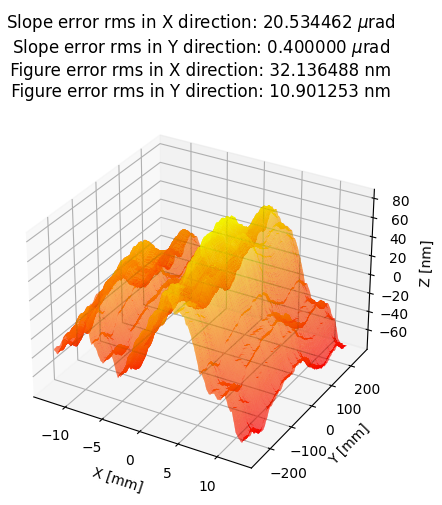
\includegraphics[width=\linewidth]{./../figures/slope_error/surface_error_profile_500x25_04x20urad.png}
  %\caption{A really Awesome Image}\label{fig:awesome_image3}
\endminipage
\caption{\label{fig:fractals} Modified mirror surfaces. }
\end{figure}

\subsection{Substrates slope error}
For this paragraph a substrate length of 500 mm is considered.

\subsubsection{Raytracing}
\begin{wrapfigure}{r}{0.3\linewidth}
\centering
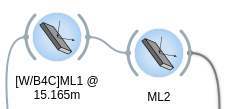
\includegraphics[width=0.3\textwidth]{images/DMM_oasys.png}
\caption{\label{fig:DMM_oasys} Double Multilayer Monochromator in Oasys Shadow.}
\end{wrapfigure}

The double-bounce DMM is modelled with two Shadow Plane Mirror widgets in series (Figure \ref{fig:DMM_oasys}). ML reflectivity is modelled with a Shadow PreMLayer widget as shown in Figure \ref{fig:PreMLayer}. The mirror surface is modified with Surface Error external splines with varying longitudinal slope error (0.1, 0.2, 0.3, 0.4 and 0.5 $\mu rad$ RMS). These modified surfaces (\ref{fig:fractals}) are simulated with the Shadow PreProcessor - Height Profile Simulator widget. The transversal slope error is kept constant at 20 $\mu rad$ RMS and fractal profiles are chosen. 

\begin{figure}  % spans both columns
\begin{subfigure}{0.5\textwidth}
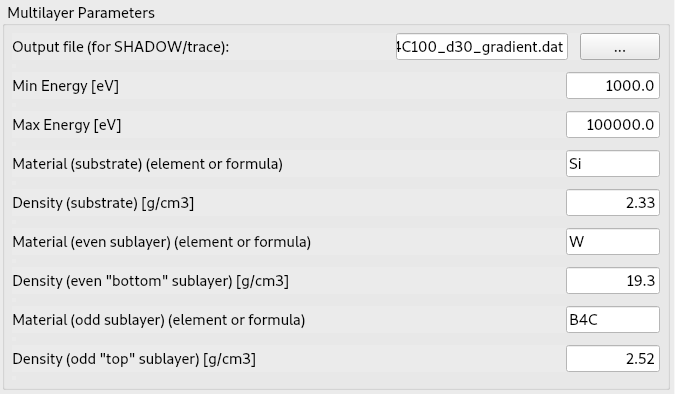
\includegraphics[width=\linewidth]{images/MLspecs_a.png}
\end{subfigure}
\hfill % maximize the horizontal distance between the graphs
\begin{subfigure}{0.5\textwidth}
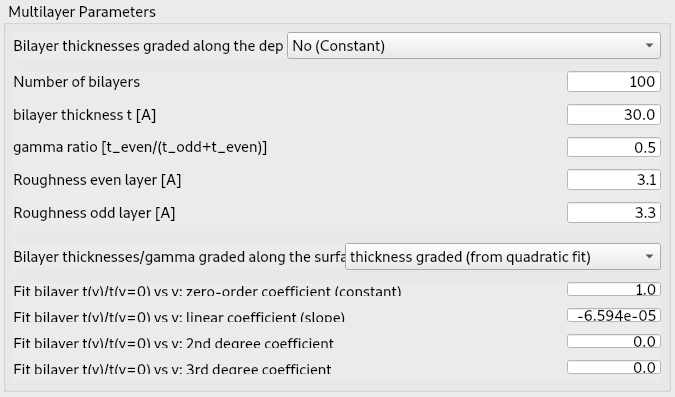
\includegraphics[width=\linewidth]{images/MLspecs_b.png}
\end{subfigure}
\caption{\label{fig:PreMLayer} PreMLayer widget settings in Shadow. }
\end{figure}

\begin{figure}[!htb]
\minipage{0.32\textwidth}
  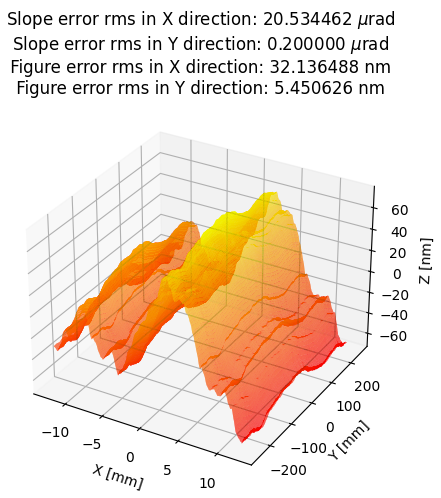
\includegraphics[width=\linewidth]{./../figures/slope_error/surface_error_profile_500x25_02x20urad.png}
  % \caption{A really Awesome Image}\label{fig:awesome_image1}
\endminipage\hfill
\minipage{0.32\textwidth}
  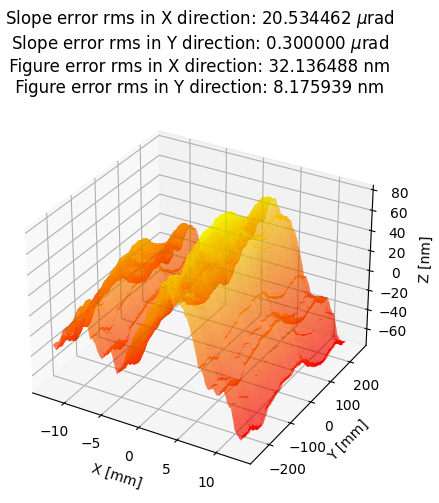
\includegraphics[width=\linewidth]{./../figures/slope_error/surface_error_profile_500x25_03x20urad.png}
  % \caption{A really Awesome Image}\label{fig:awesome_image2}
\endminipage\hfill
\minipage{0.32\textwidth}%
  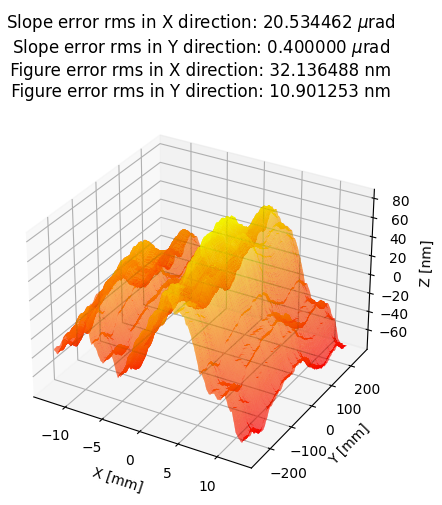
\includegraphics[width=\linewidth]{./../figures/slope_error/surface_error_profile_500x25_04x20urad.png}
  %\caption{A really Awesome Image}\label{fig:awesome_image3}
\endminipage
\caption{\label{fig:fractals} Modified mirror surfaces. }
\end{figure}

%%%%%%%%%%%%%%%%%%%%%%%%%%%%%%%%%%%%%%%%%%%%%%%%%%%%%%%%%%%%%%%%%%%%%%%%%%%%%%%%%%
\clearpage
\subsubsection{0.1 urad}
\begin{figure}[H]
\centering
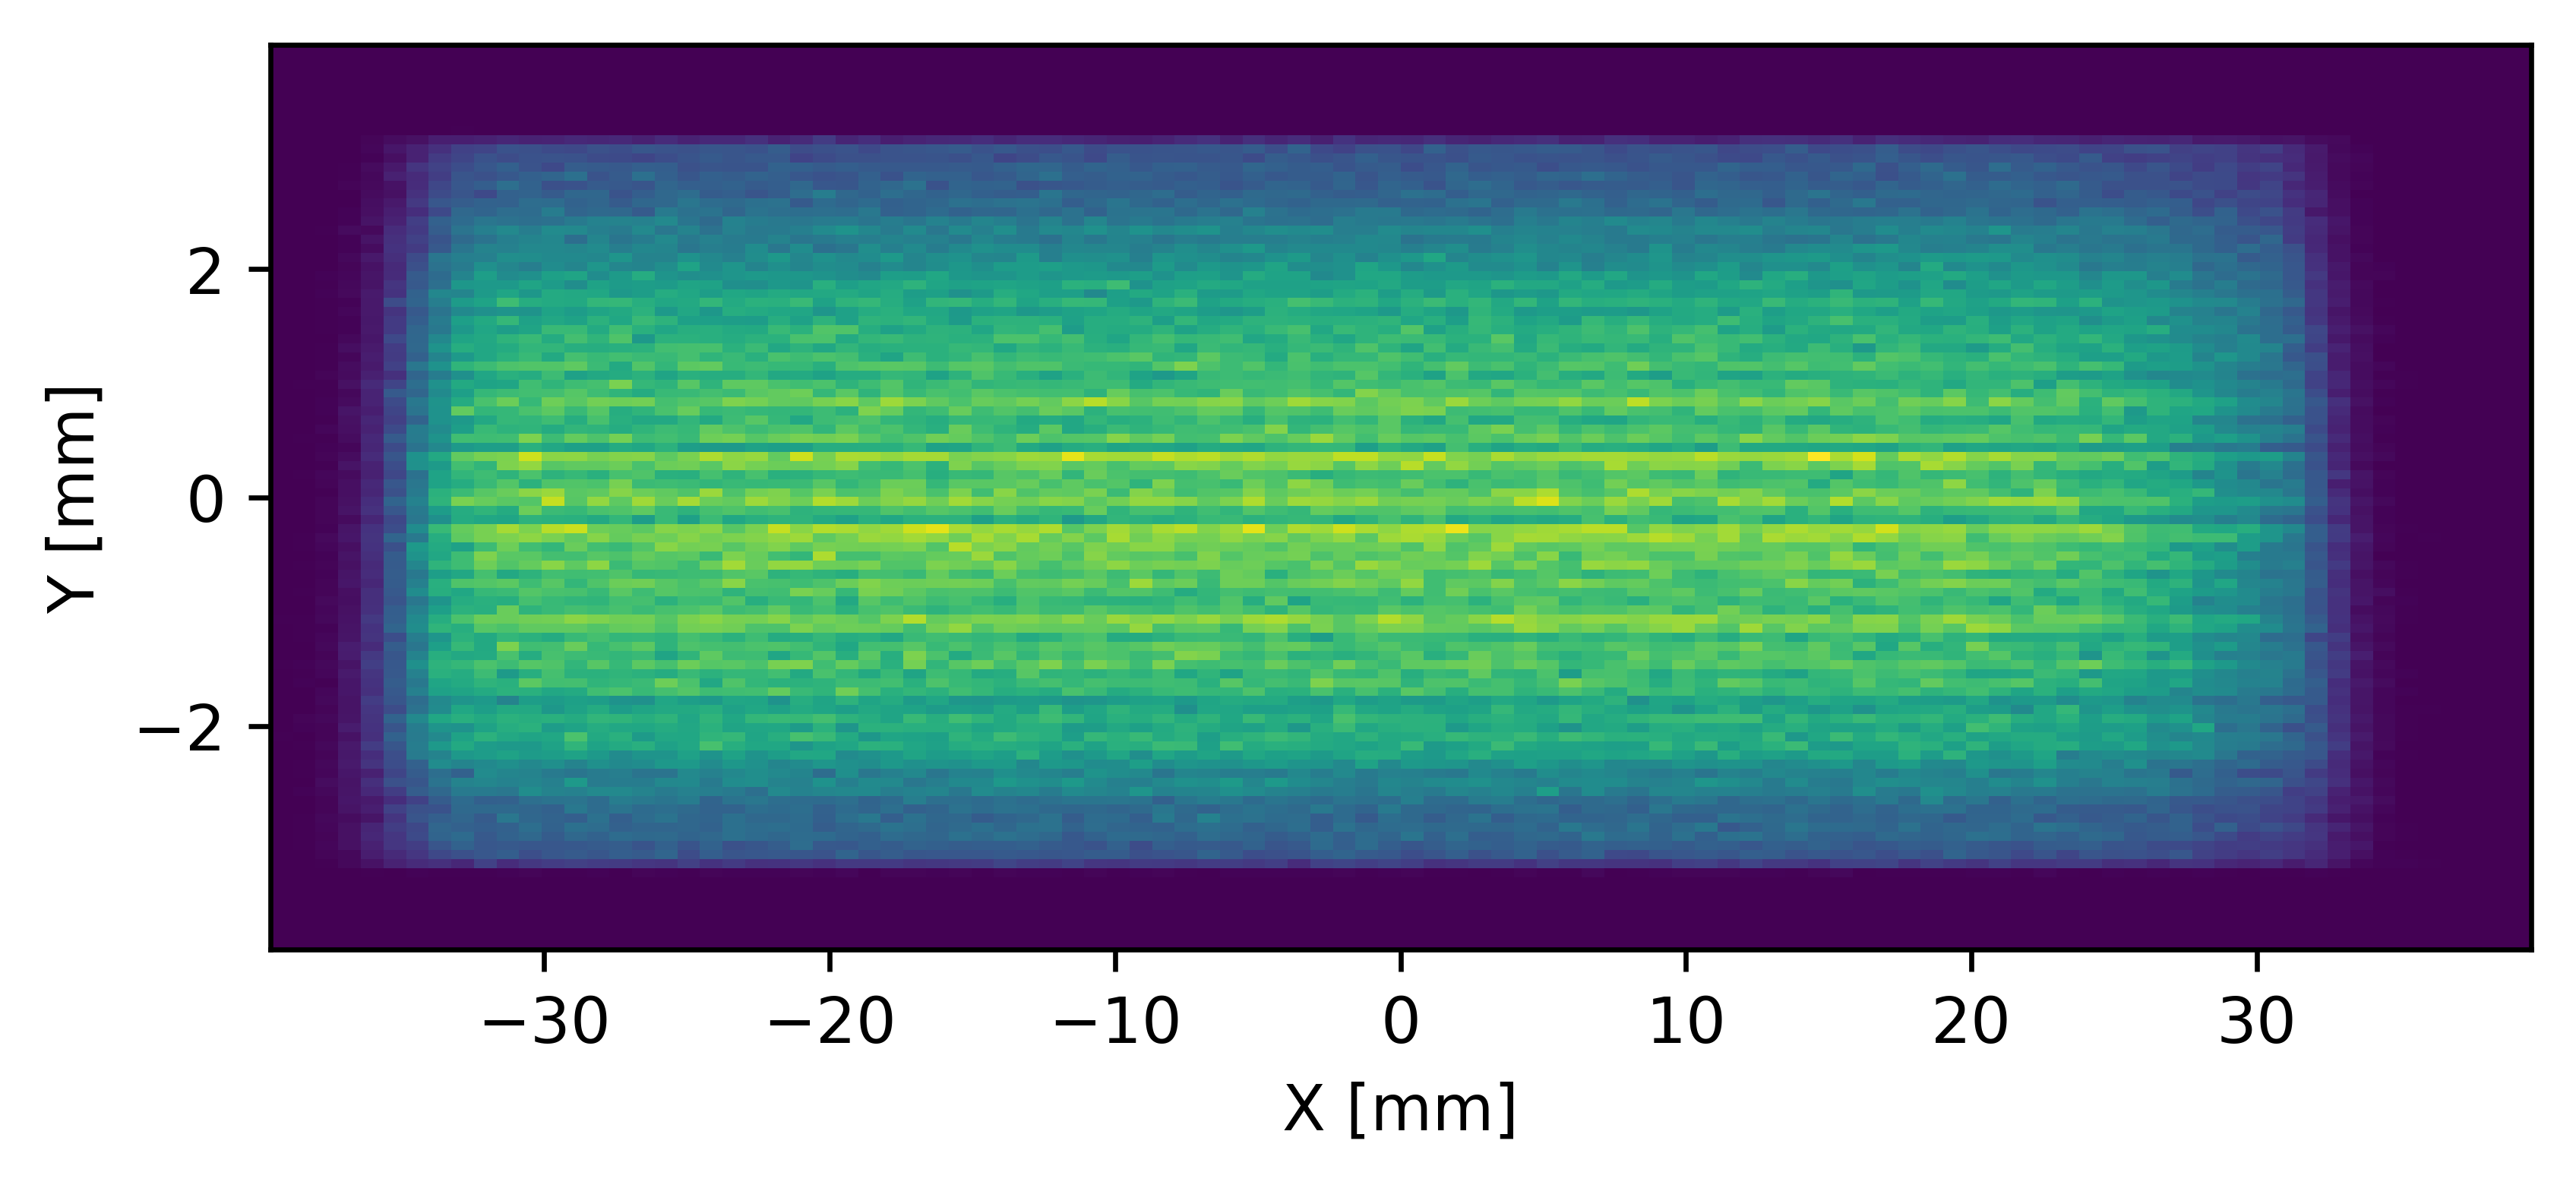
\includegraphics[width=0.9\linewidth]{./../figures/slope_error/WB4C_d30_d-spacing_gradient_45keV_slope_error01urad.png}
\end{figure}

\begin{figure}[H]
\centering
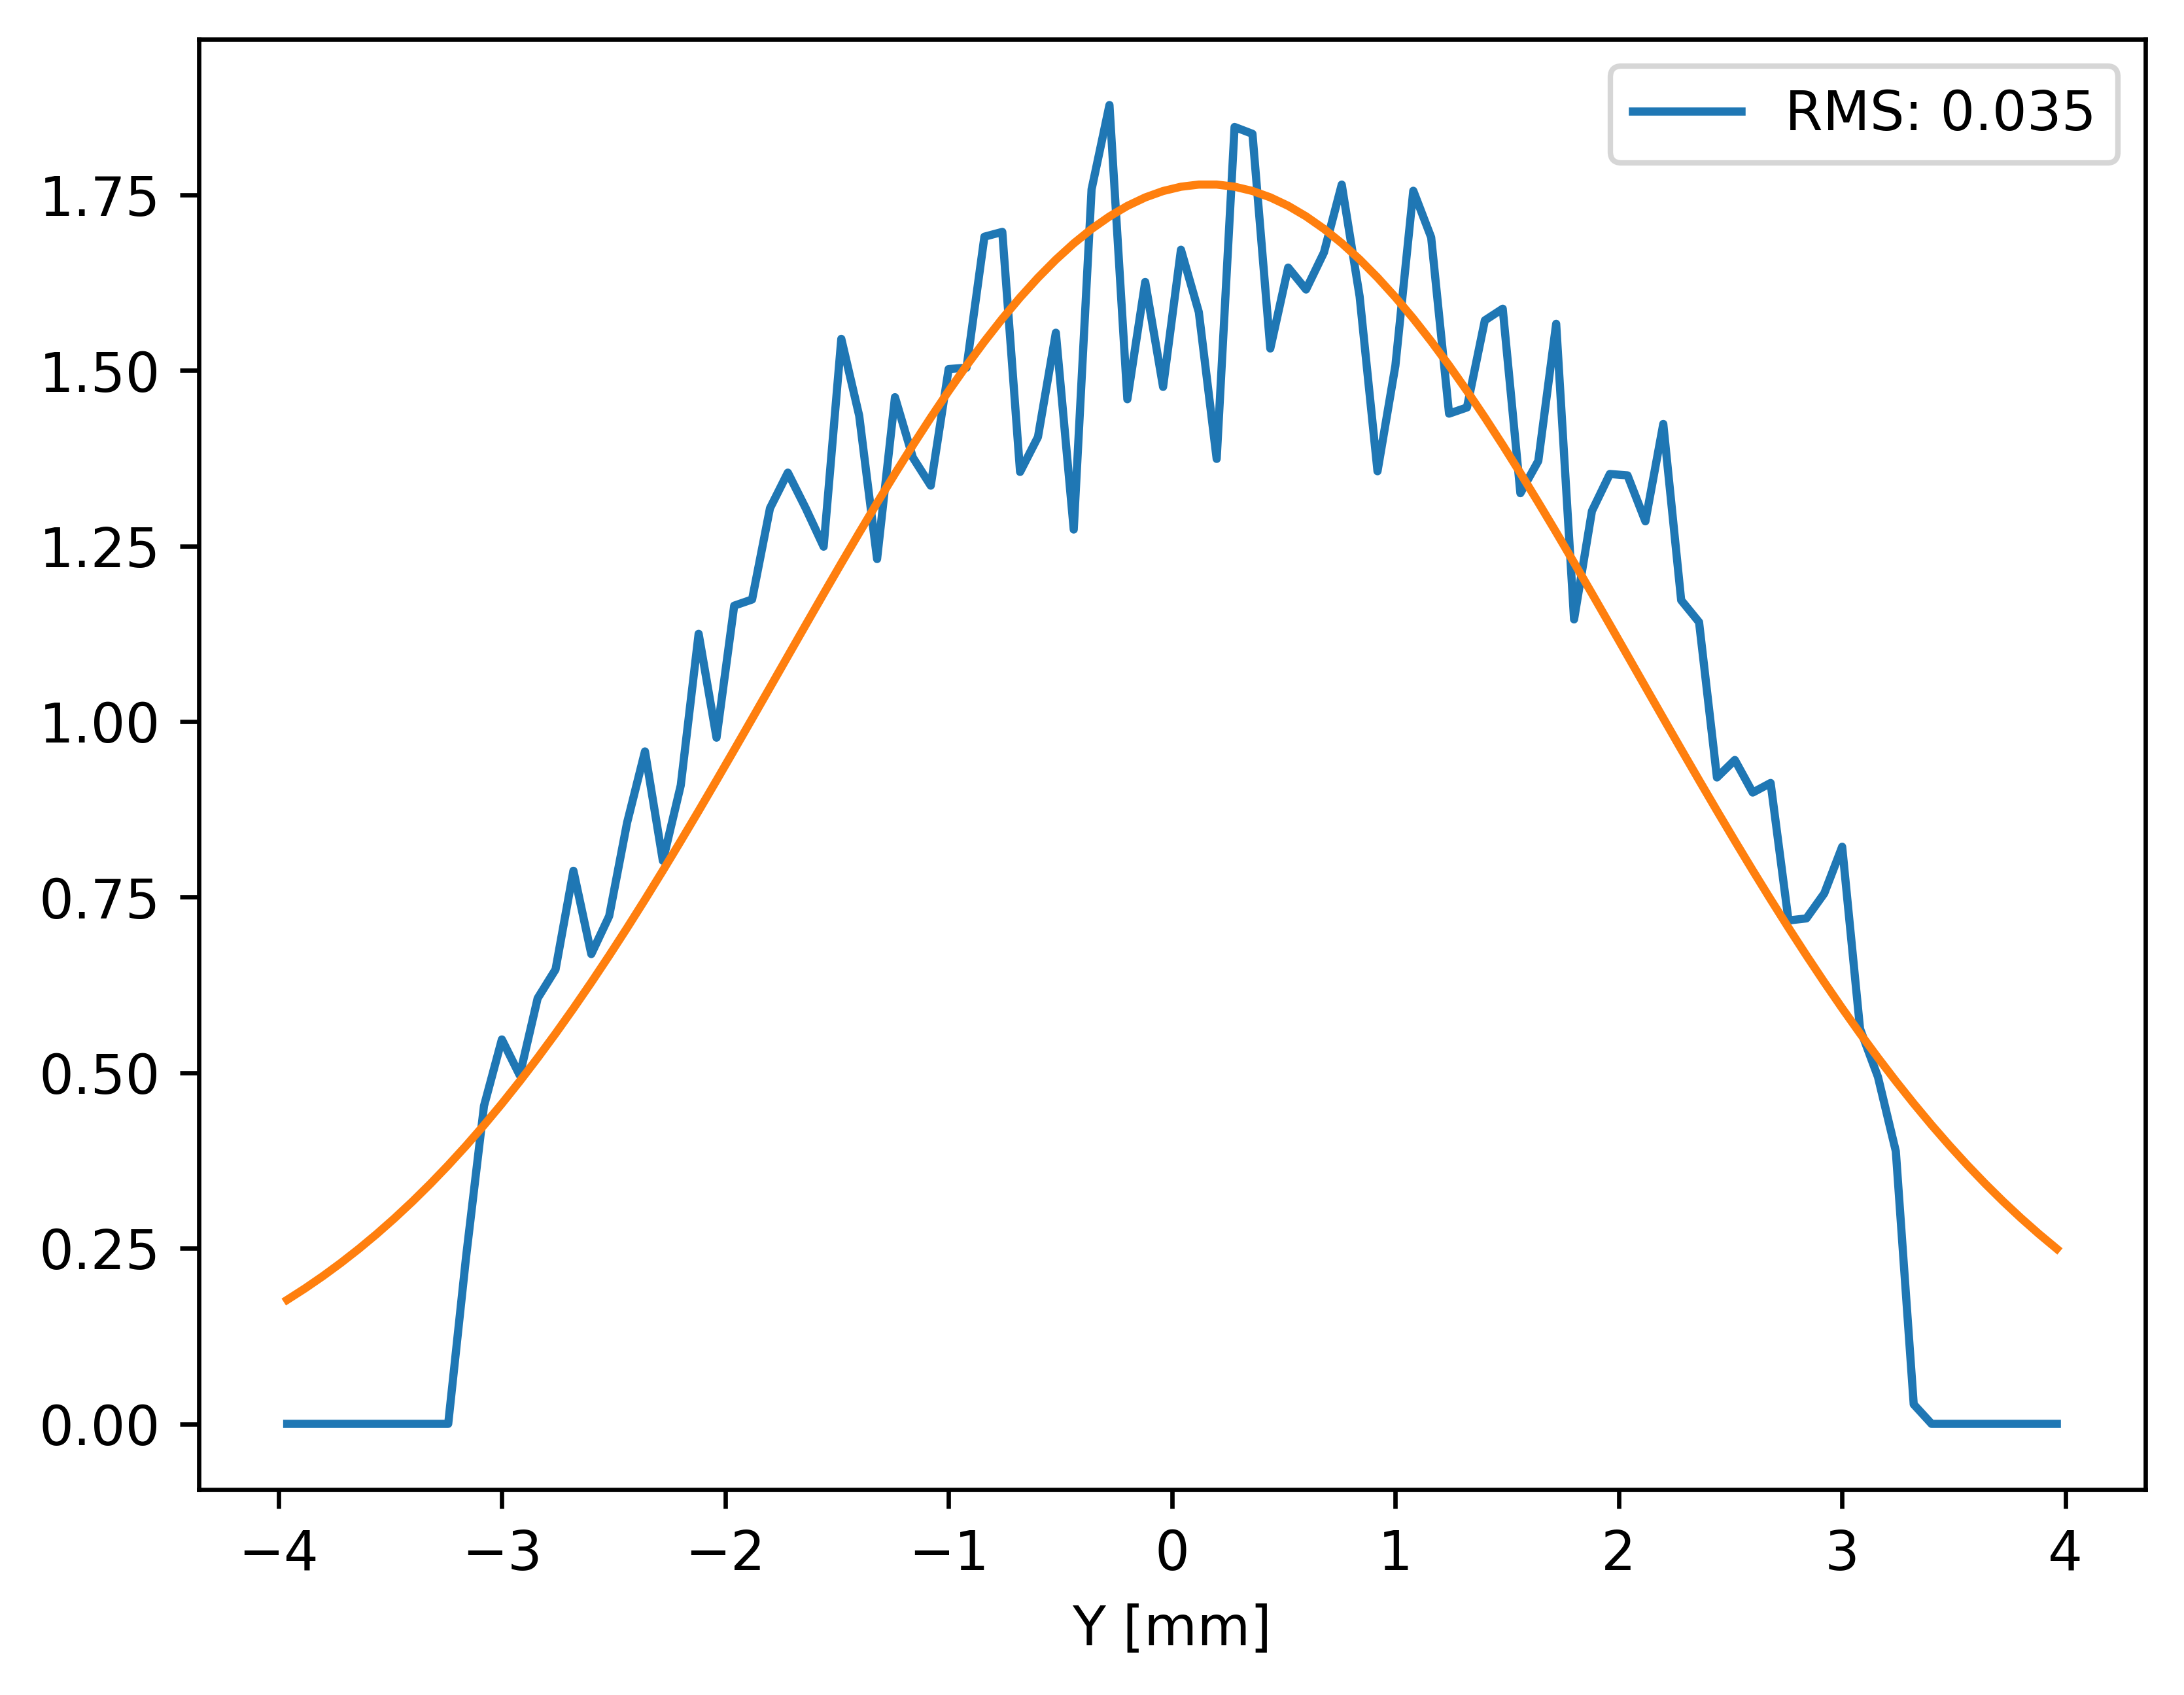
\includegraphics[width=0.9\linewidth]{./../figures/slope_error/WB4C_d30_d-spacing_gradient_45keV_slope_error01urad_Yprofile.png}
\caption{0.1 urad}
\label{fig:01urad}
\end{figure}

%%%%%%%%%%%%%%%%%%%%%%%%%%%%%%%%%%%%%%%%%%%%%%%%%%%%%%%%%%%%%%%%%%%%%%%%%%%%%%%%%%
\clearpage
\subsubsection{0.2 urad}
\begin{figure}[H]
\centering
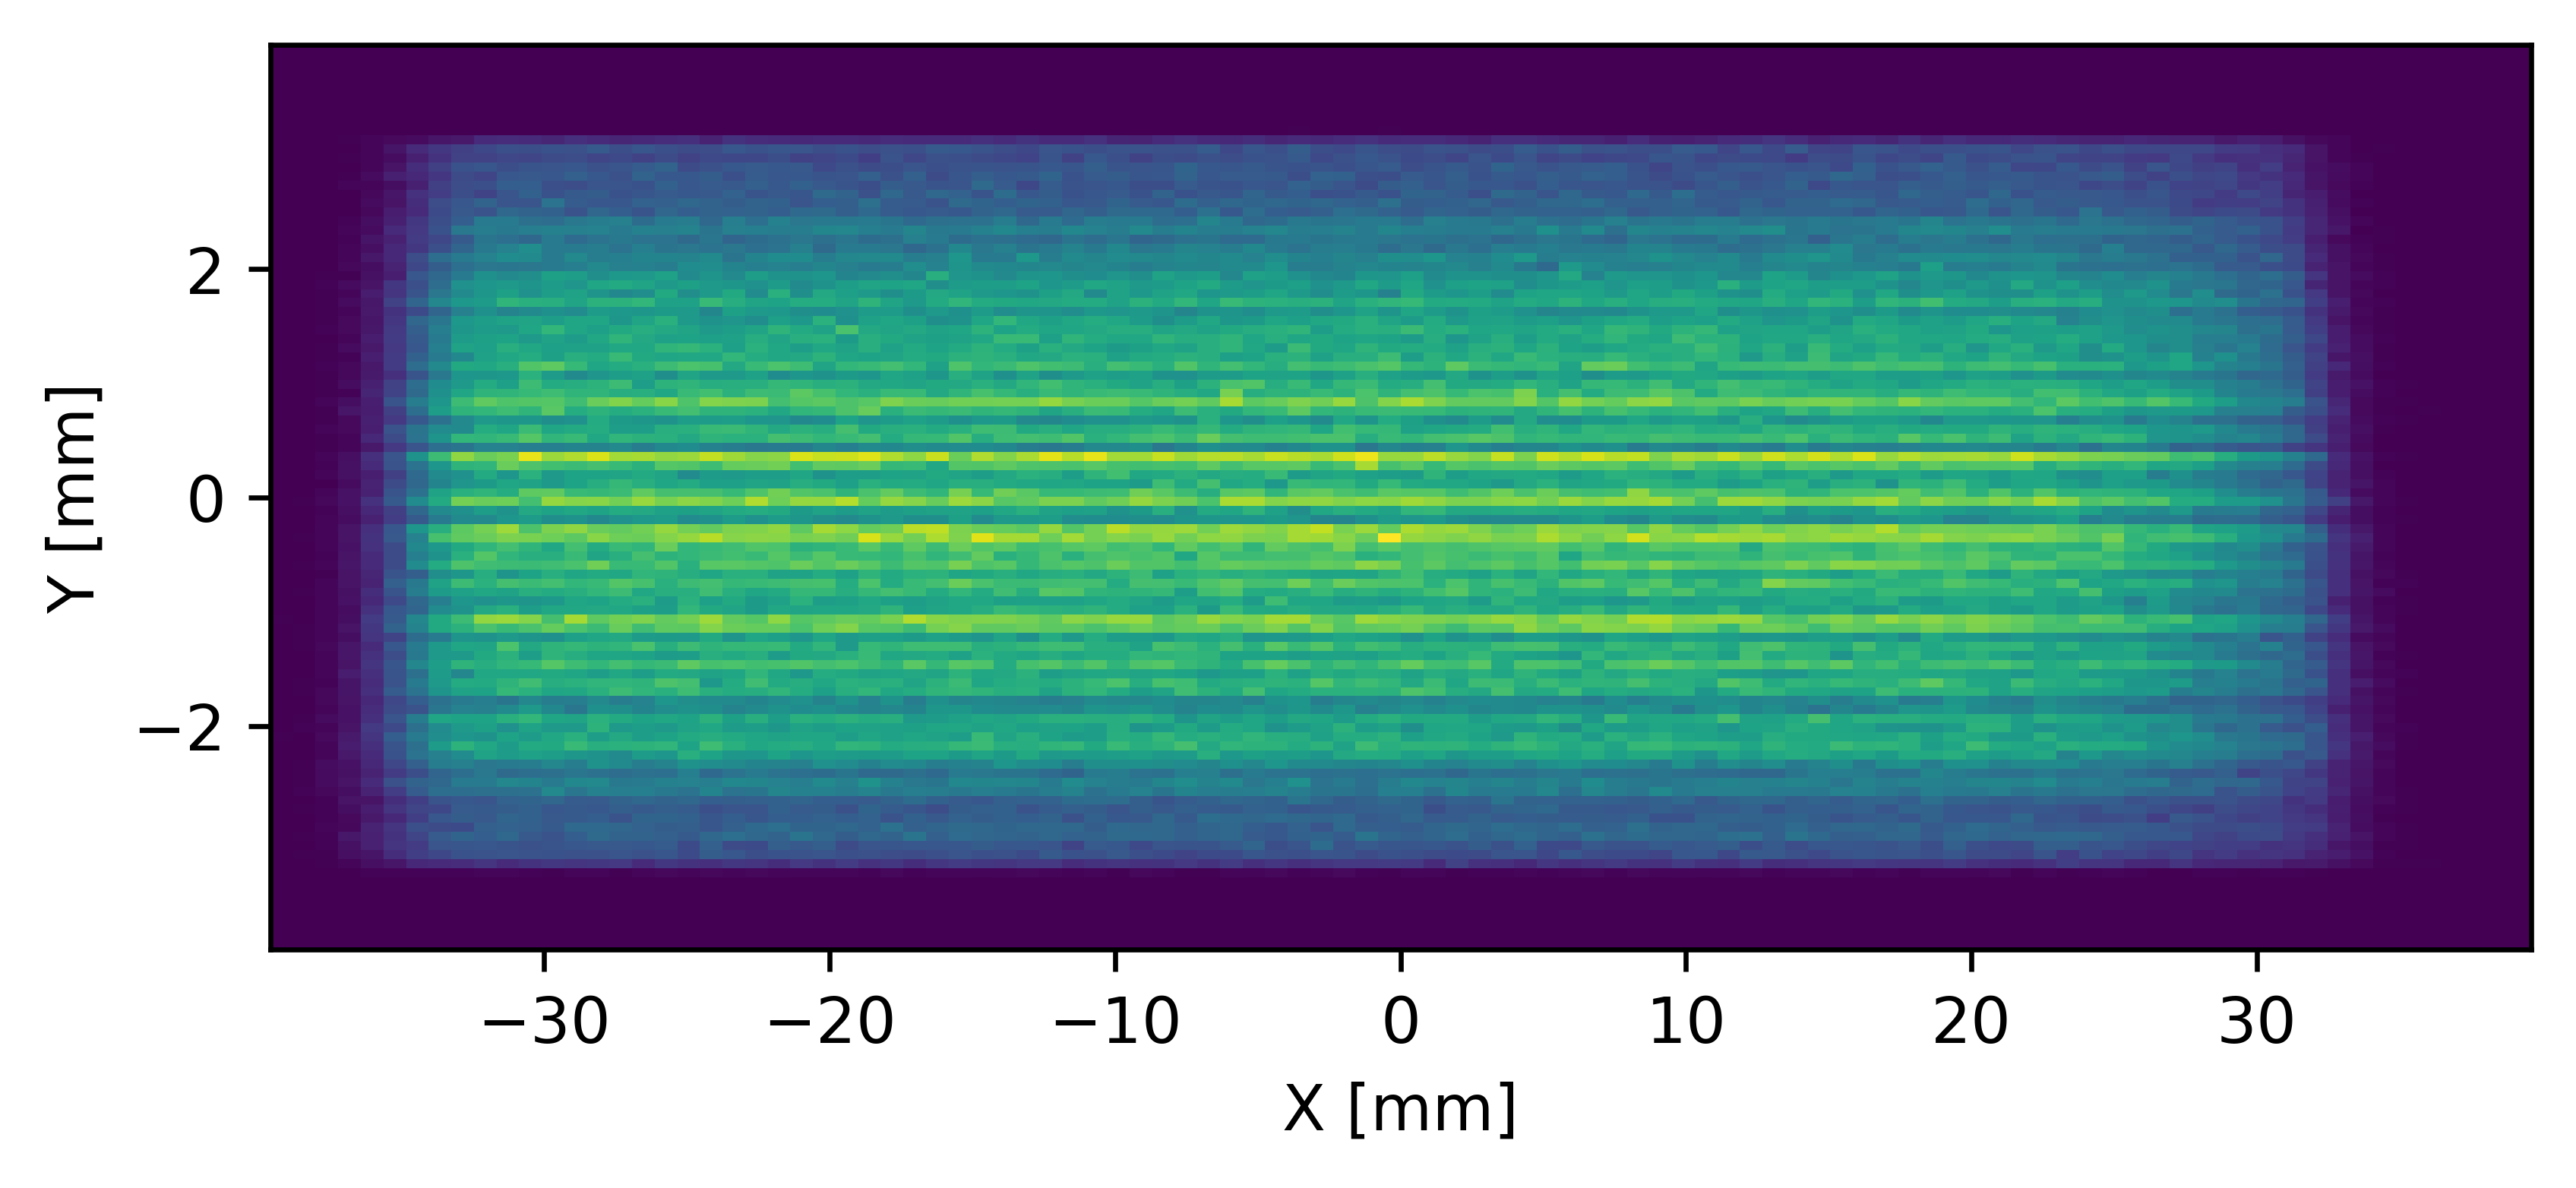
\includegraphics[width=0.9\linewidth]{./../figures/slope_error/WB4C_d30_d-spacing_gradient_45keV_slope_error02urad.png}
\end{figure}

\begin{figure}[H]
\centering
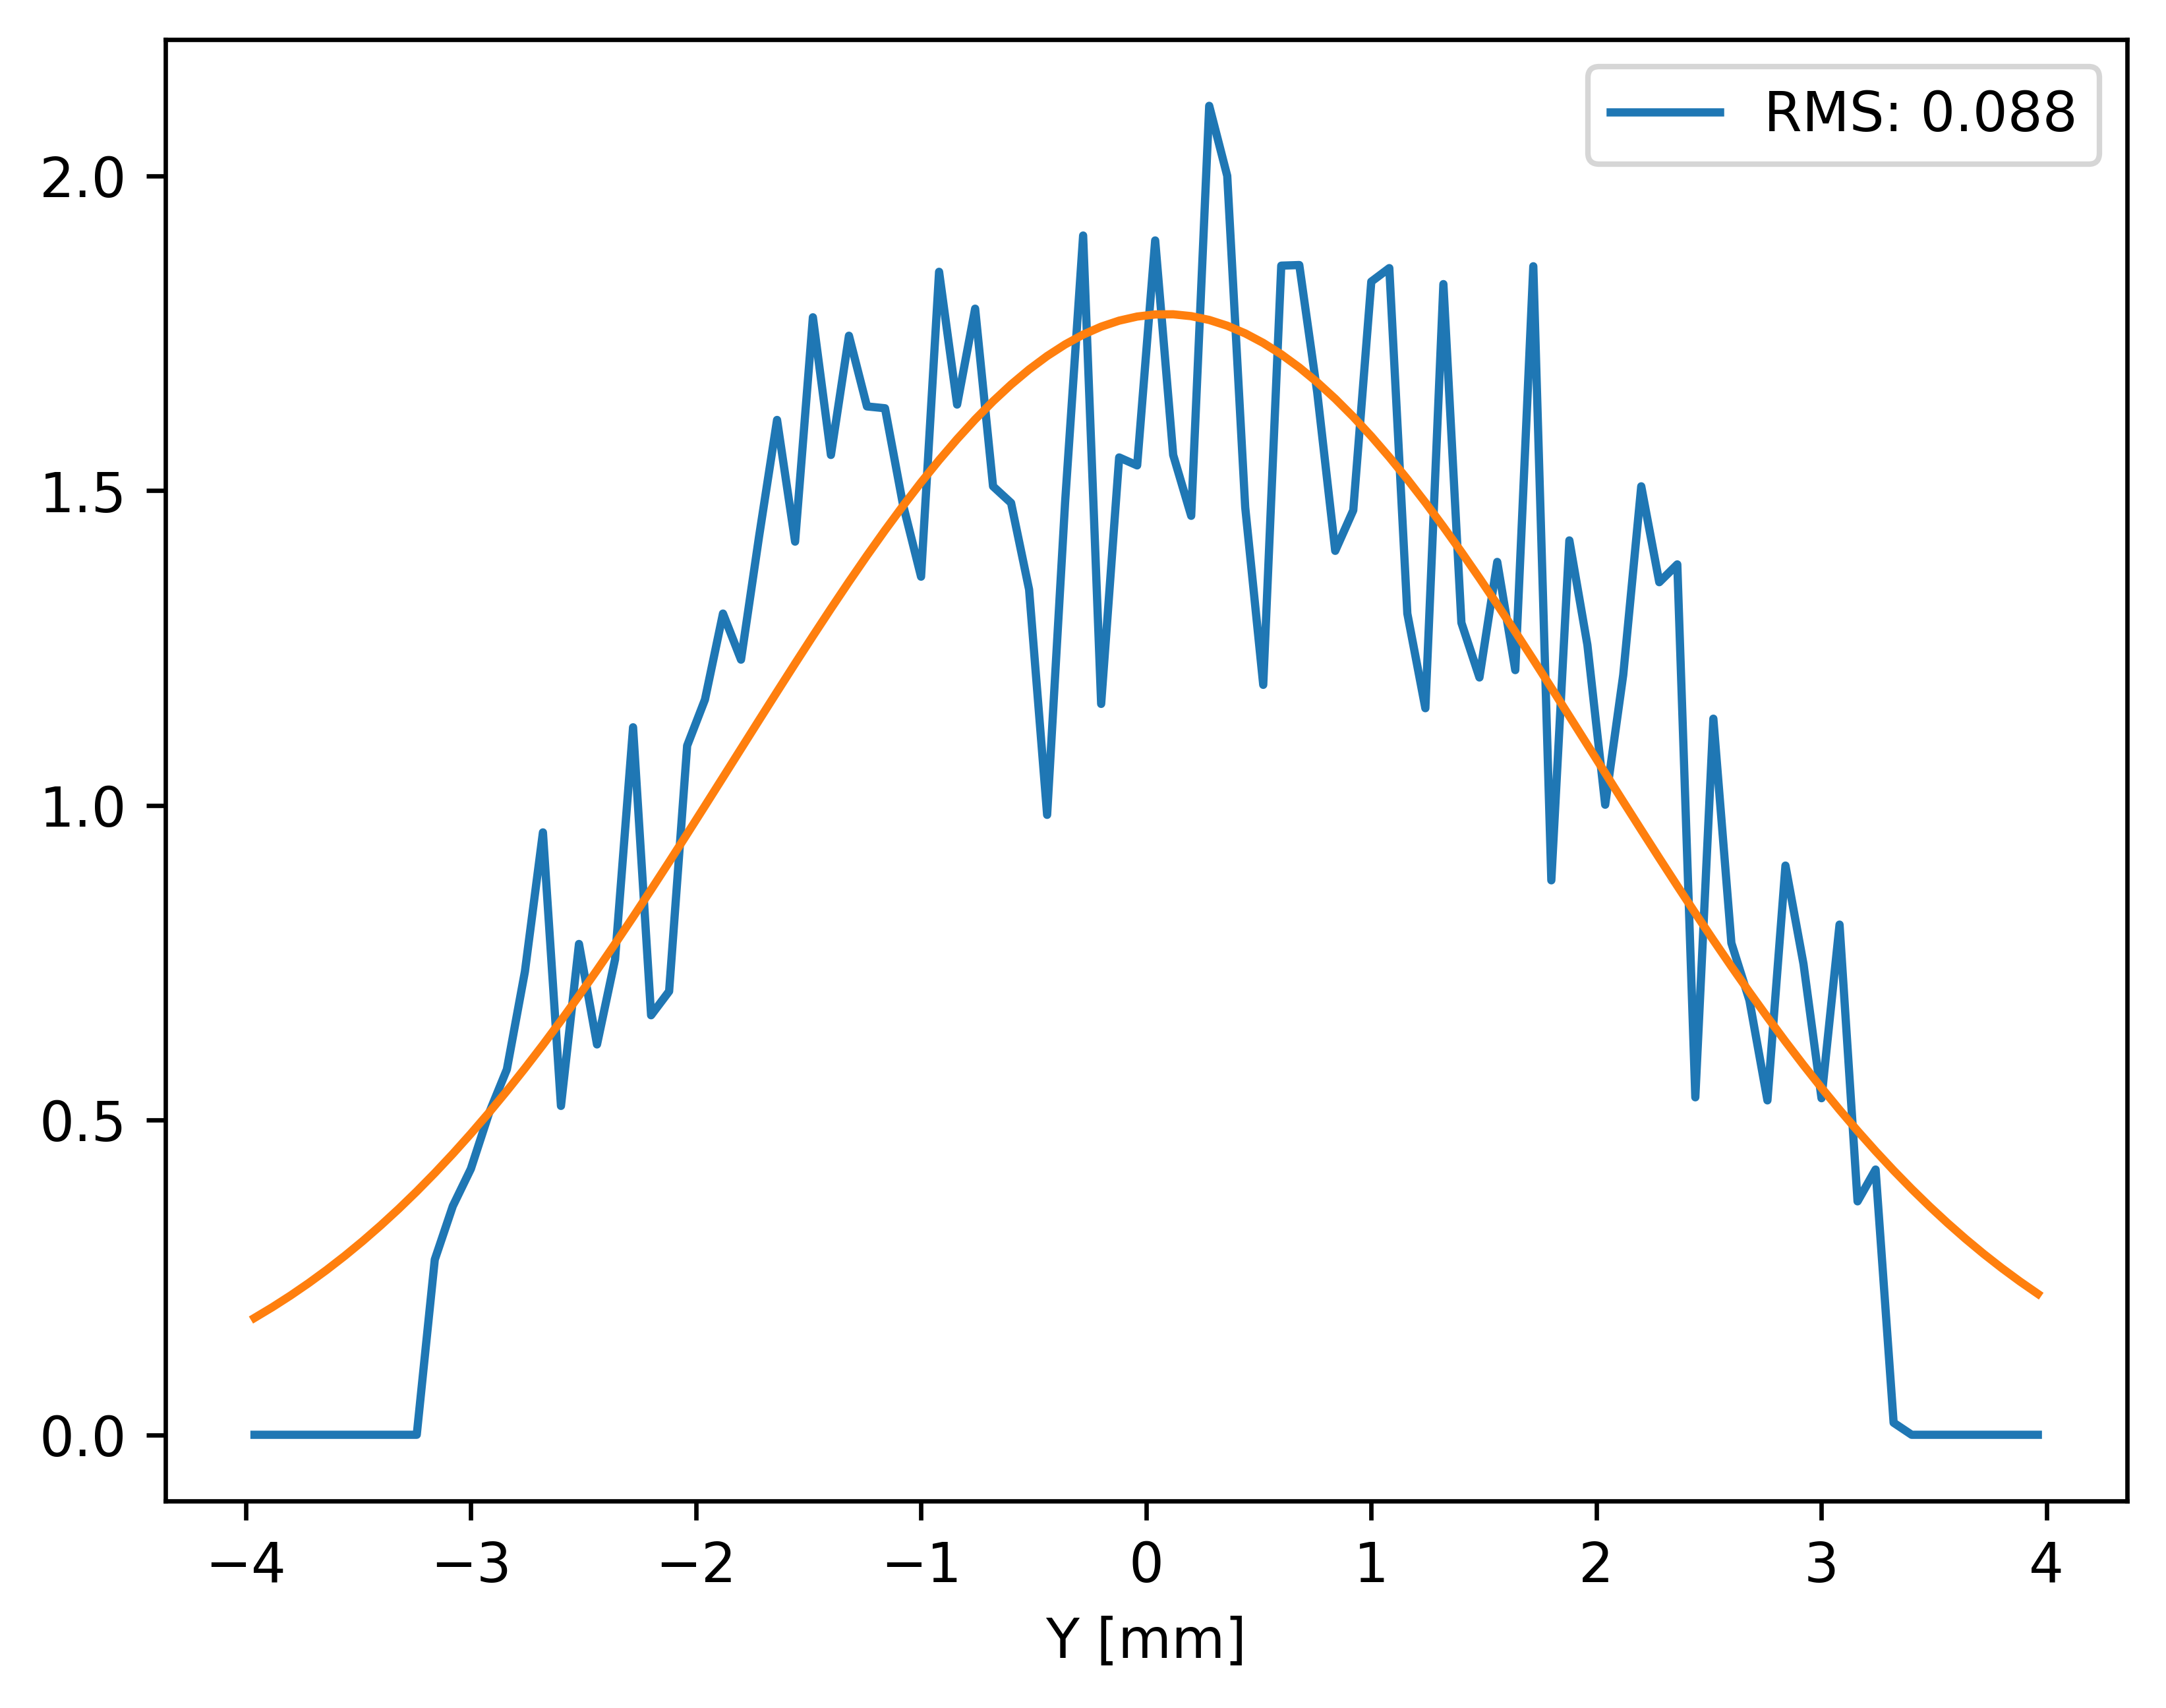
\includegraphics[width=0.9\linewidth]{./../figures/slope_error/WB4C_d30_d-spacing_gradient_45keV_slope_error02urad_Yprofile.png}
\caption{0.2 urad}
\label{fig:02urad}
\end{figure}

%%%%%%%%%%%%%%%%%%%%%%%%%%%%%%%%%%%%%%%%%%%%%%%%%%%%%%%%%%%%%%%%%%%%%%%%%%%%%%%%%%
\clearpage
\subsubsection{0.25 urad}
\begin{figure}[H]
\centering
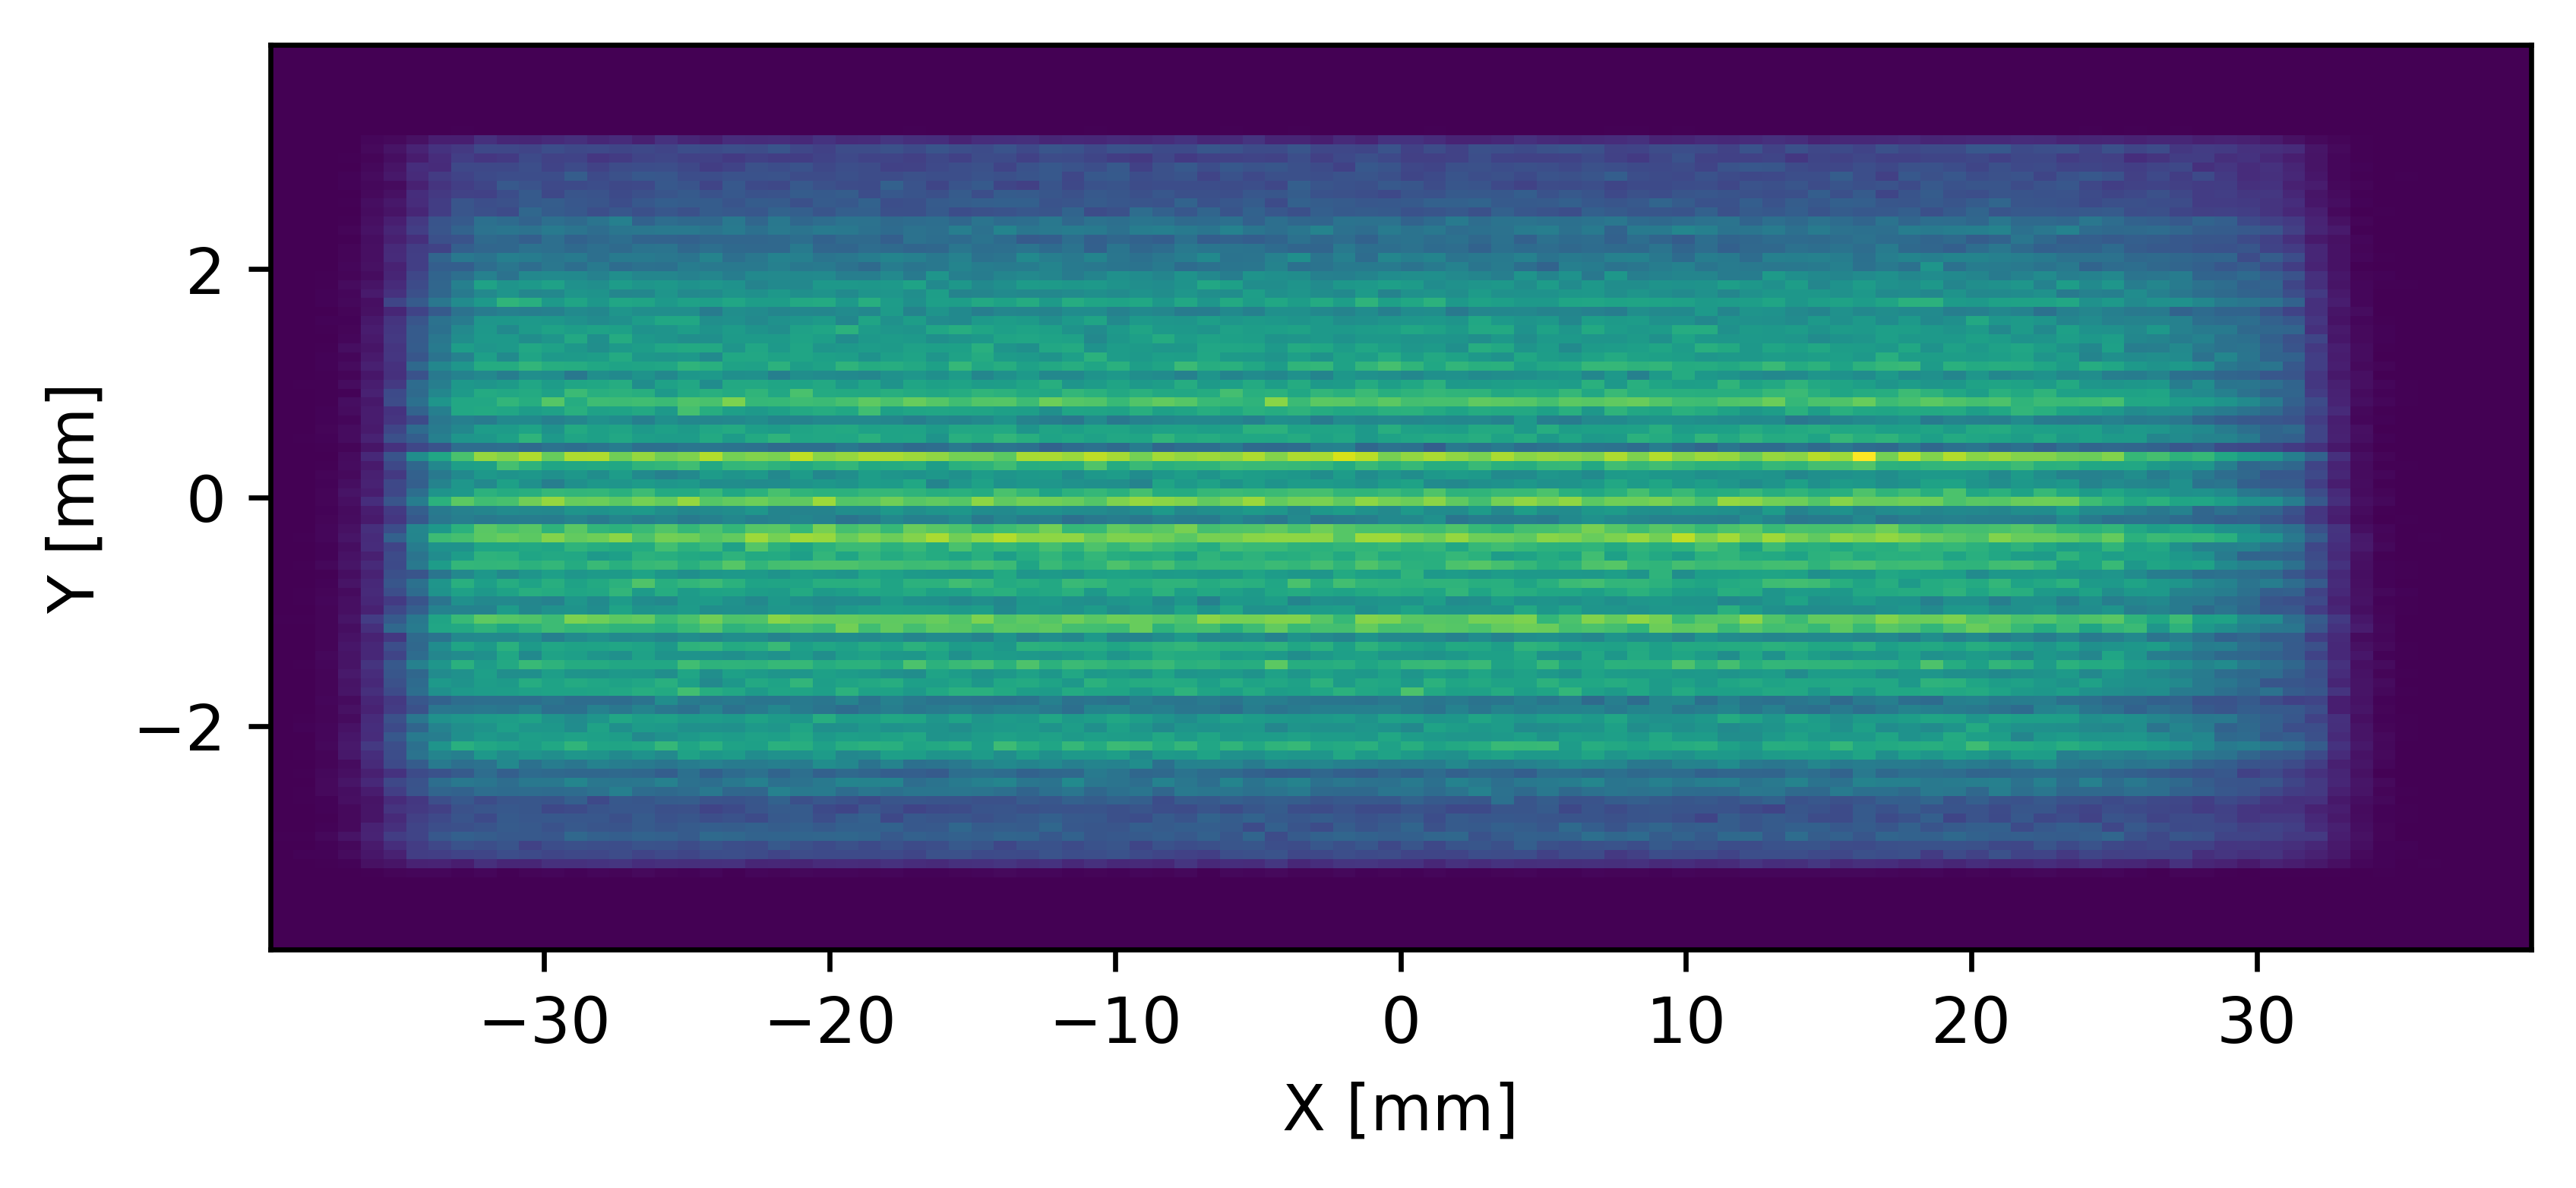
\includegraphics[width=0.9\linewidth]{./../figures/slope_error/WB4C_d30_d-spacing_gradient_45keV_slope_error025urad.png}
\end{figure}

\begin{figure}[H]
\centering
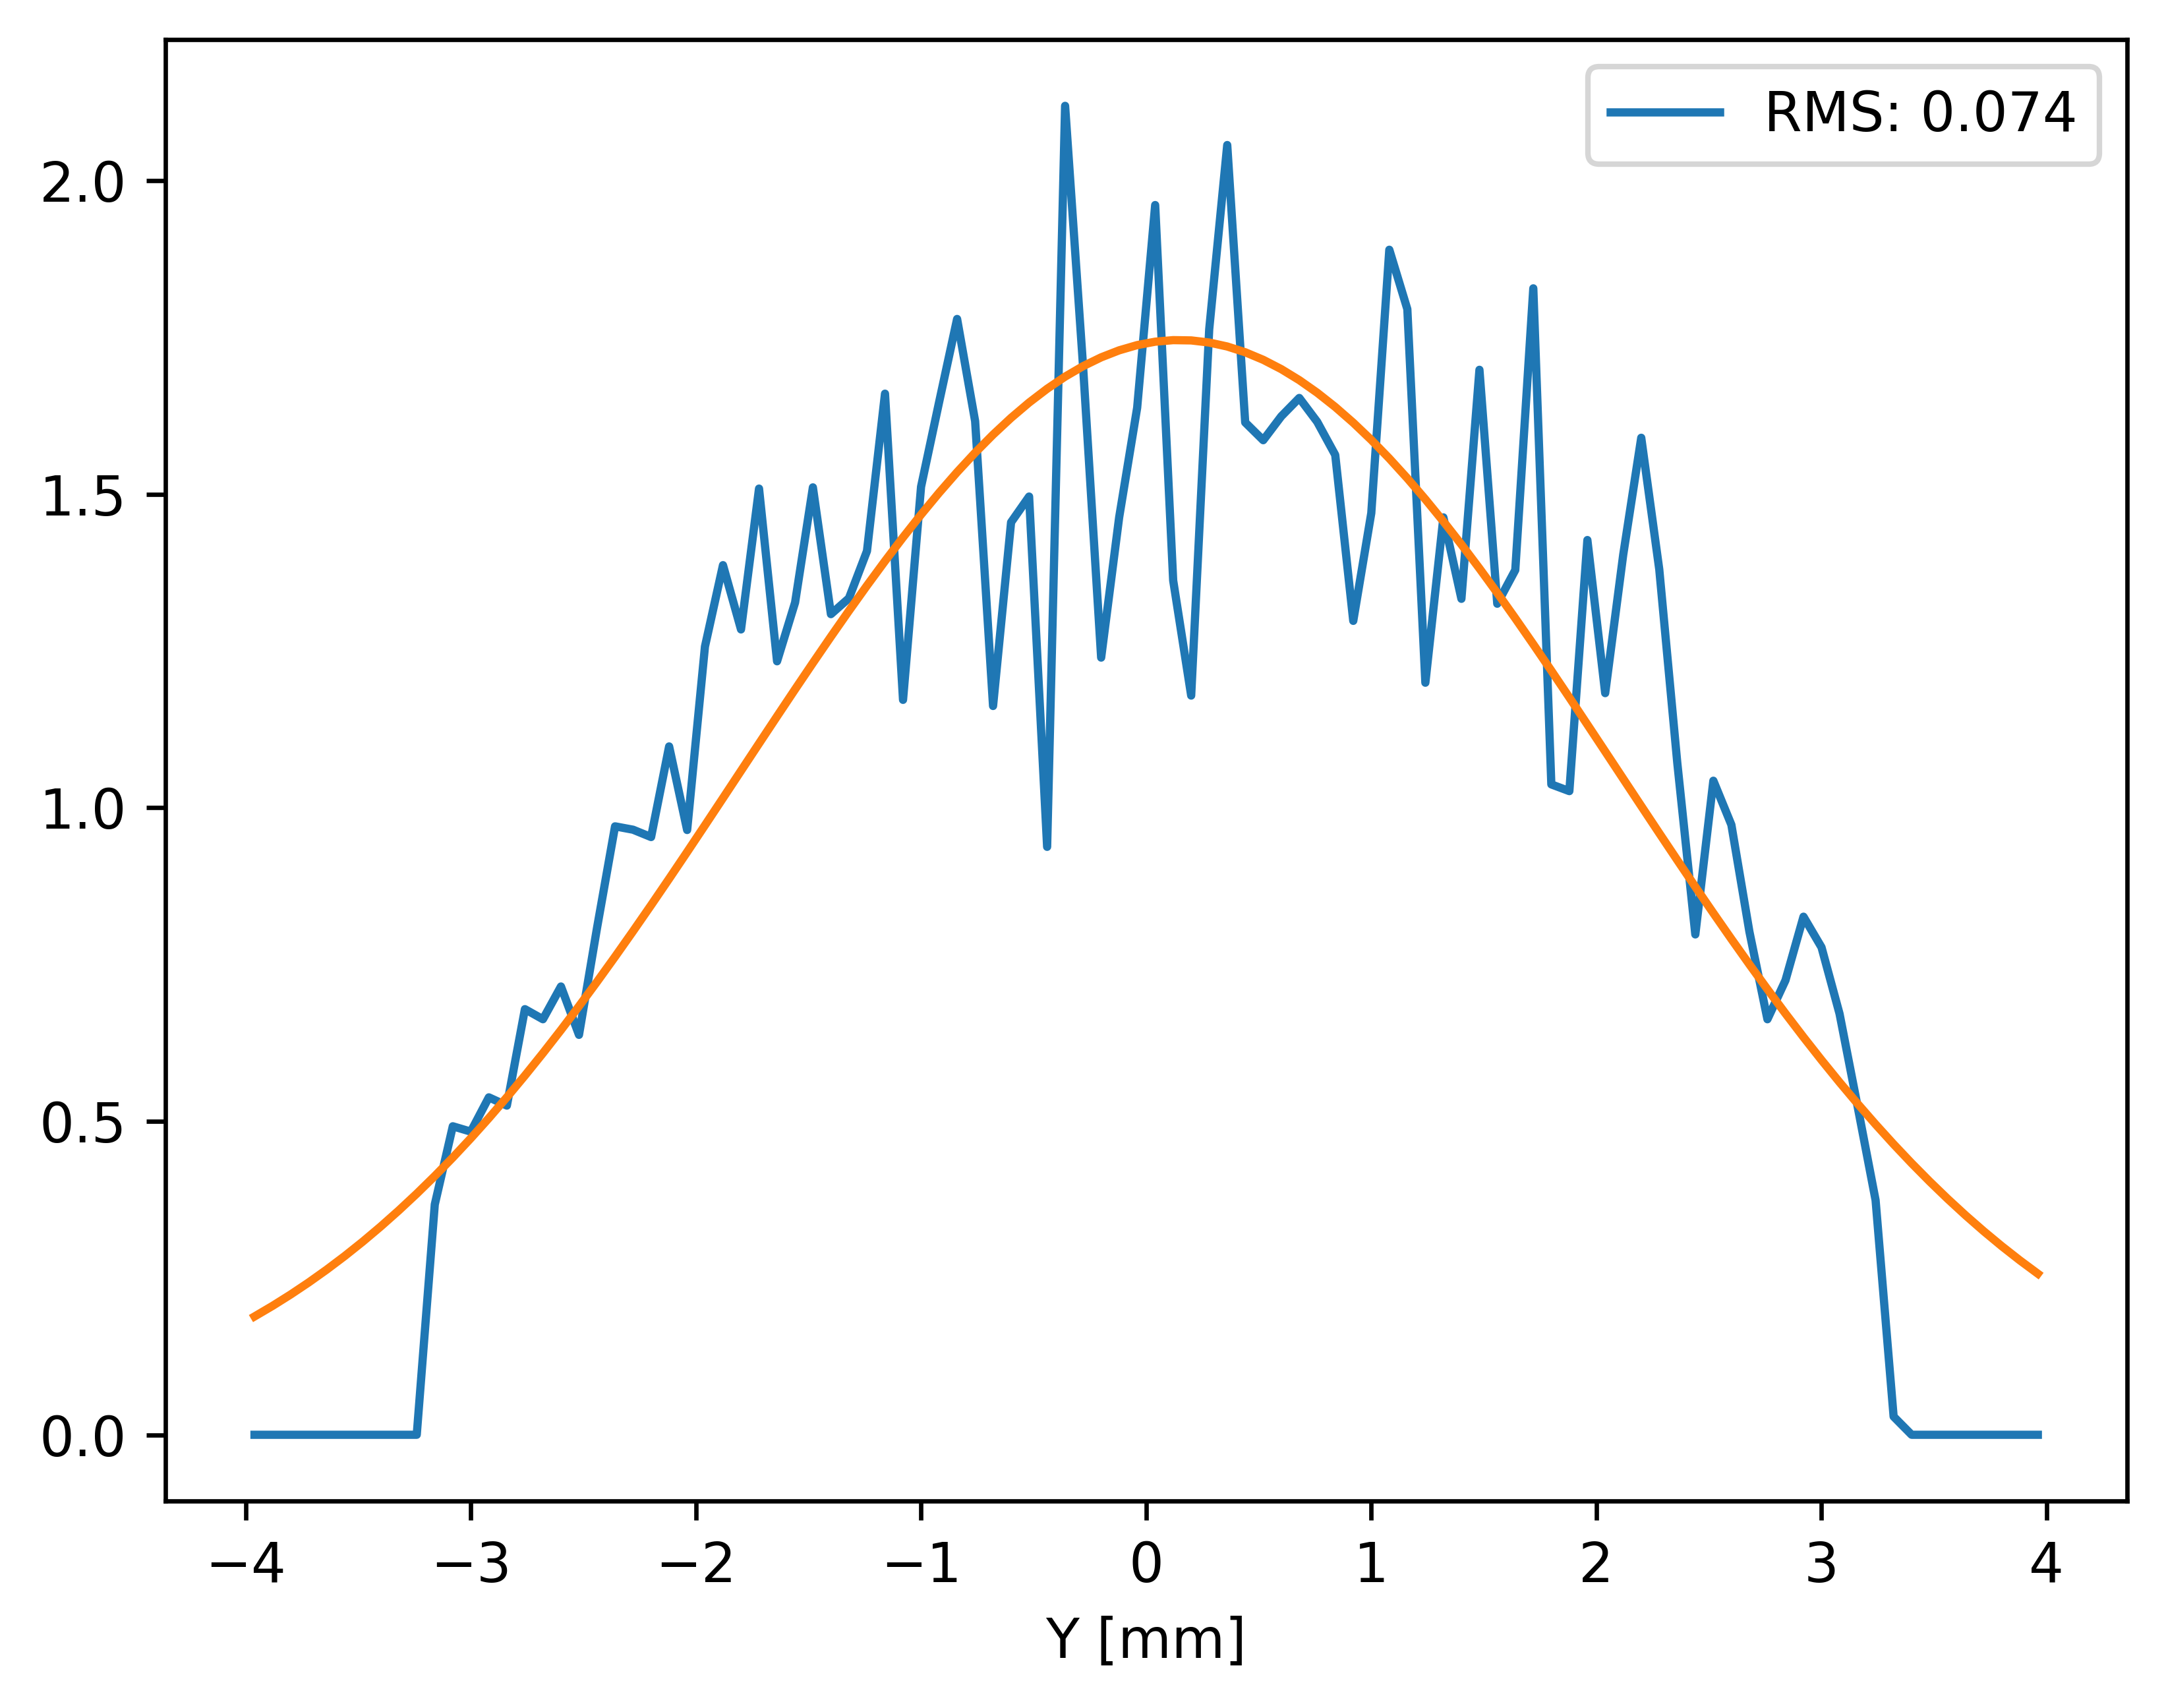
\includegraphics[width=0.9\linewidth]{./../figures/slope_error/WB4C_d30_d-spacing_gradient_45keV_slope_error025urad_Yprofile.png}
\caption{0.25 urad}
\label{fig:025urad}
\end{figure}

%%%%%%%%%%%%%%%%%%%%%%%%%%%%%%%%%%%%%%%%%%%%%%%%%%%%%%%%%%%%%%%%%%%%%%%%%%%%%%%%%%
\clearpage
\subsubsection{0.3 urad}
\begin{figure}[H]
\centering
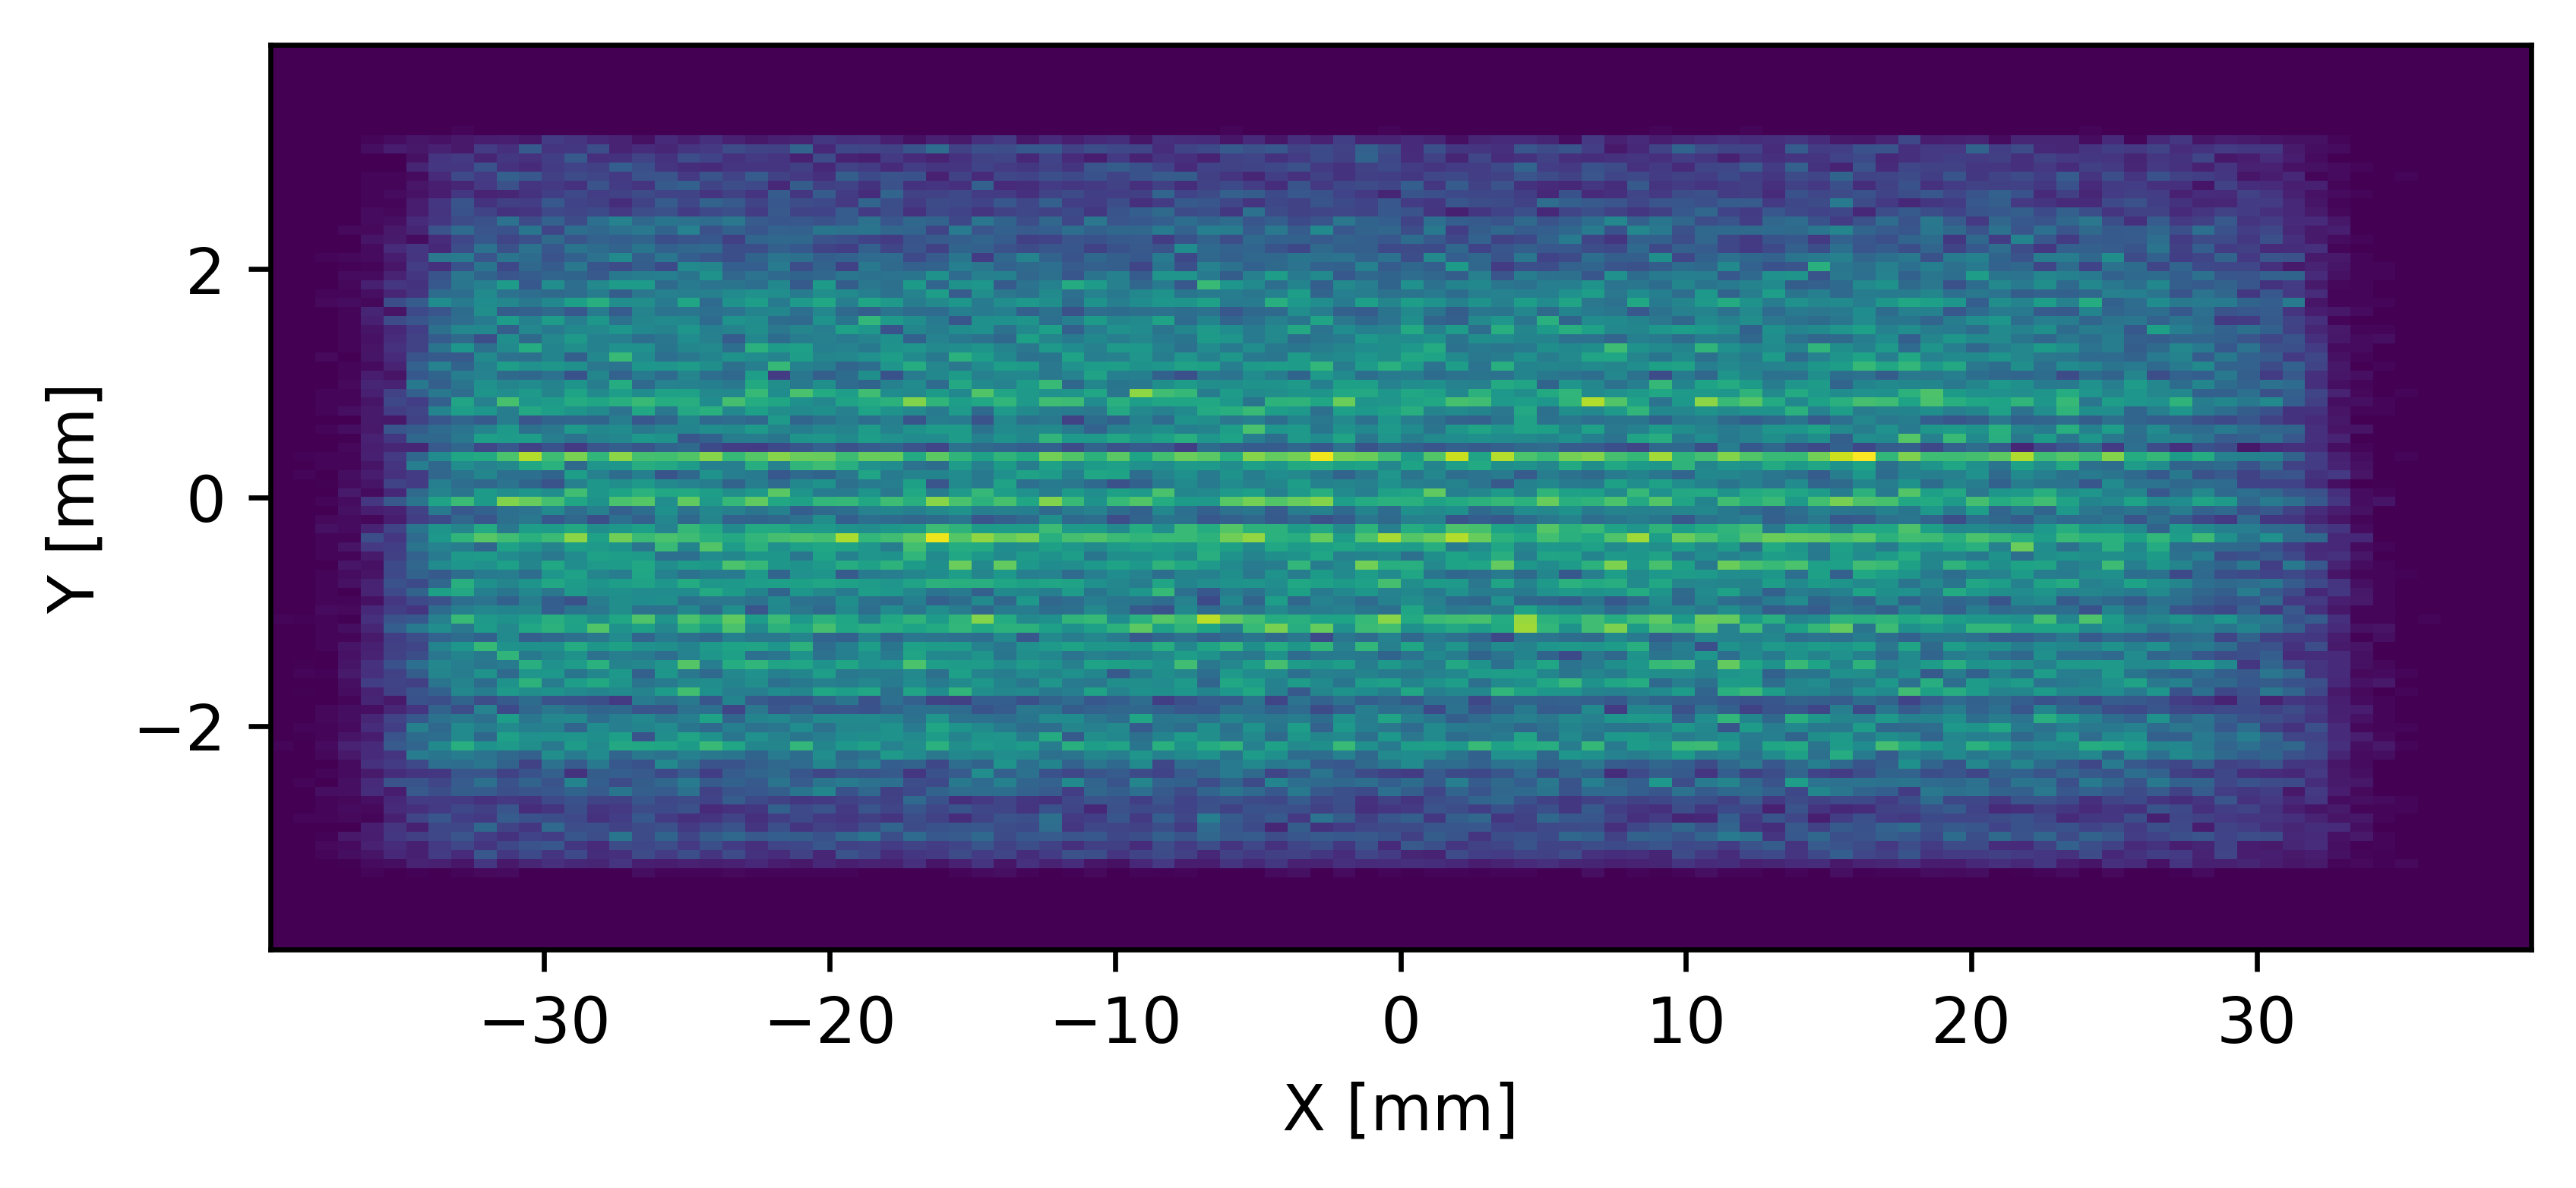
\includegraphics[width=0.9\linewidth]{./../figures/slope_error/WB4C_d30_d-spacing_gradient_45keV_slope_error03urad.png}
\end{figure}

\begin{figure}[H]
\centering
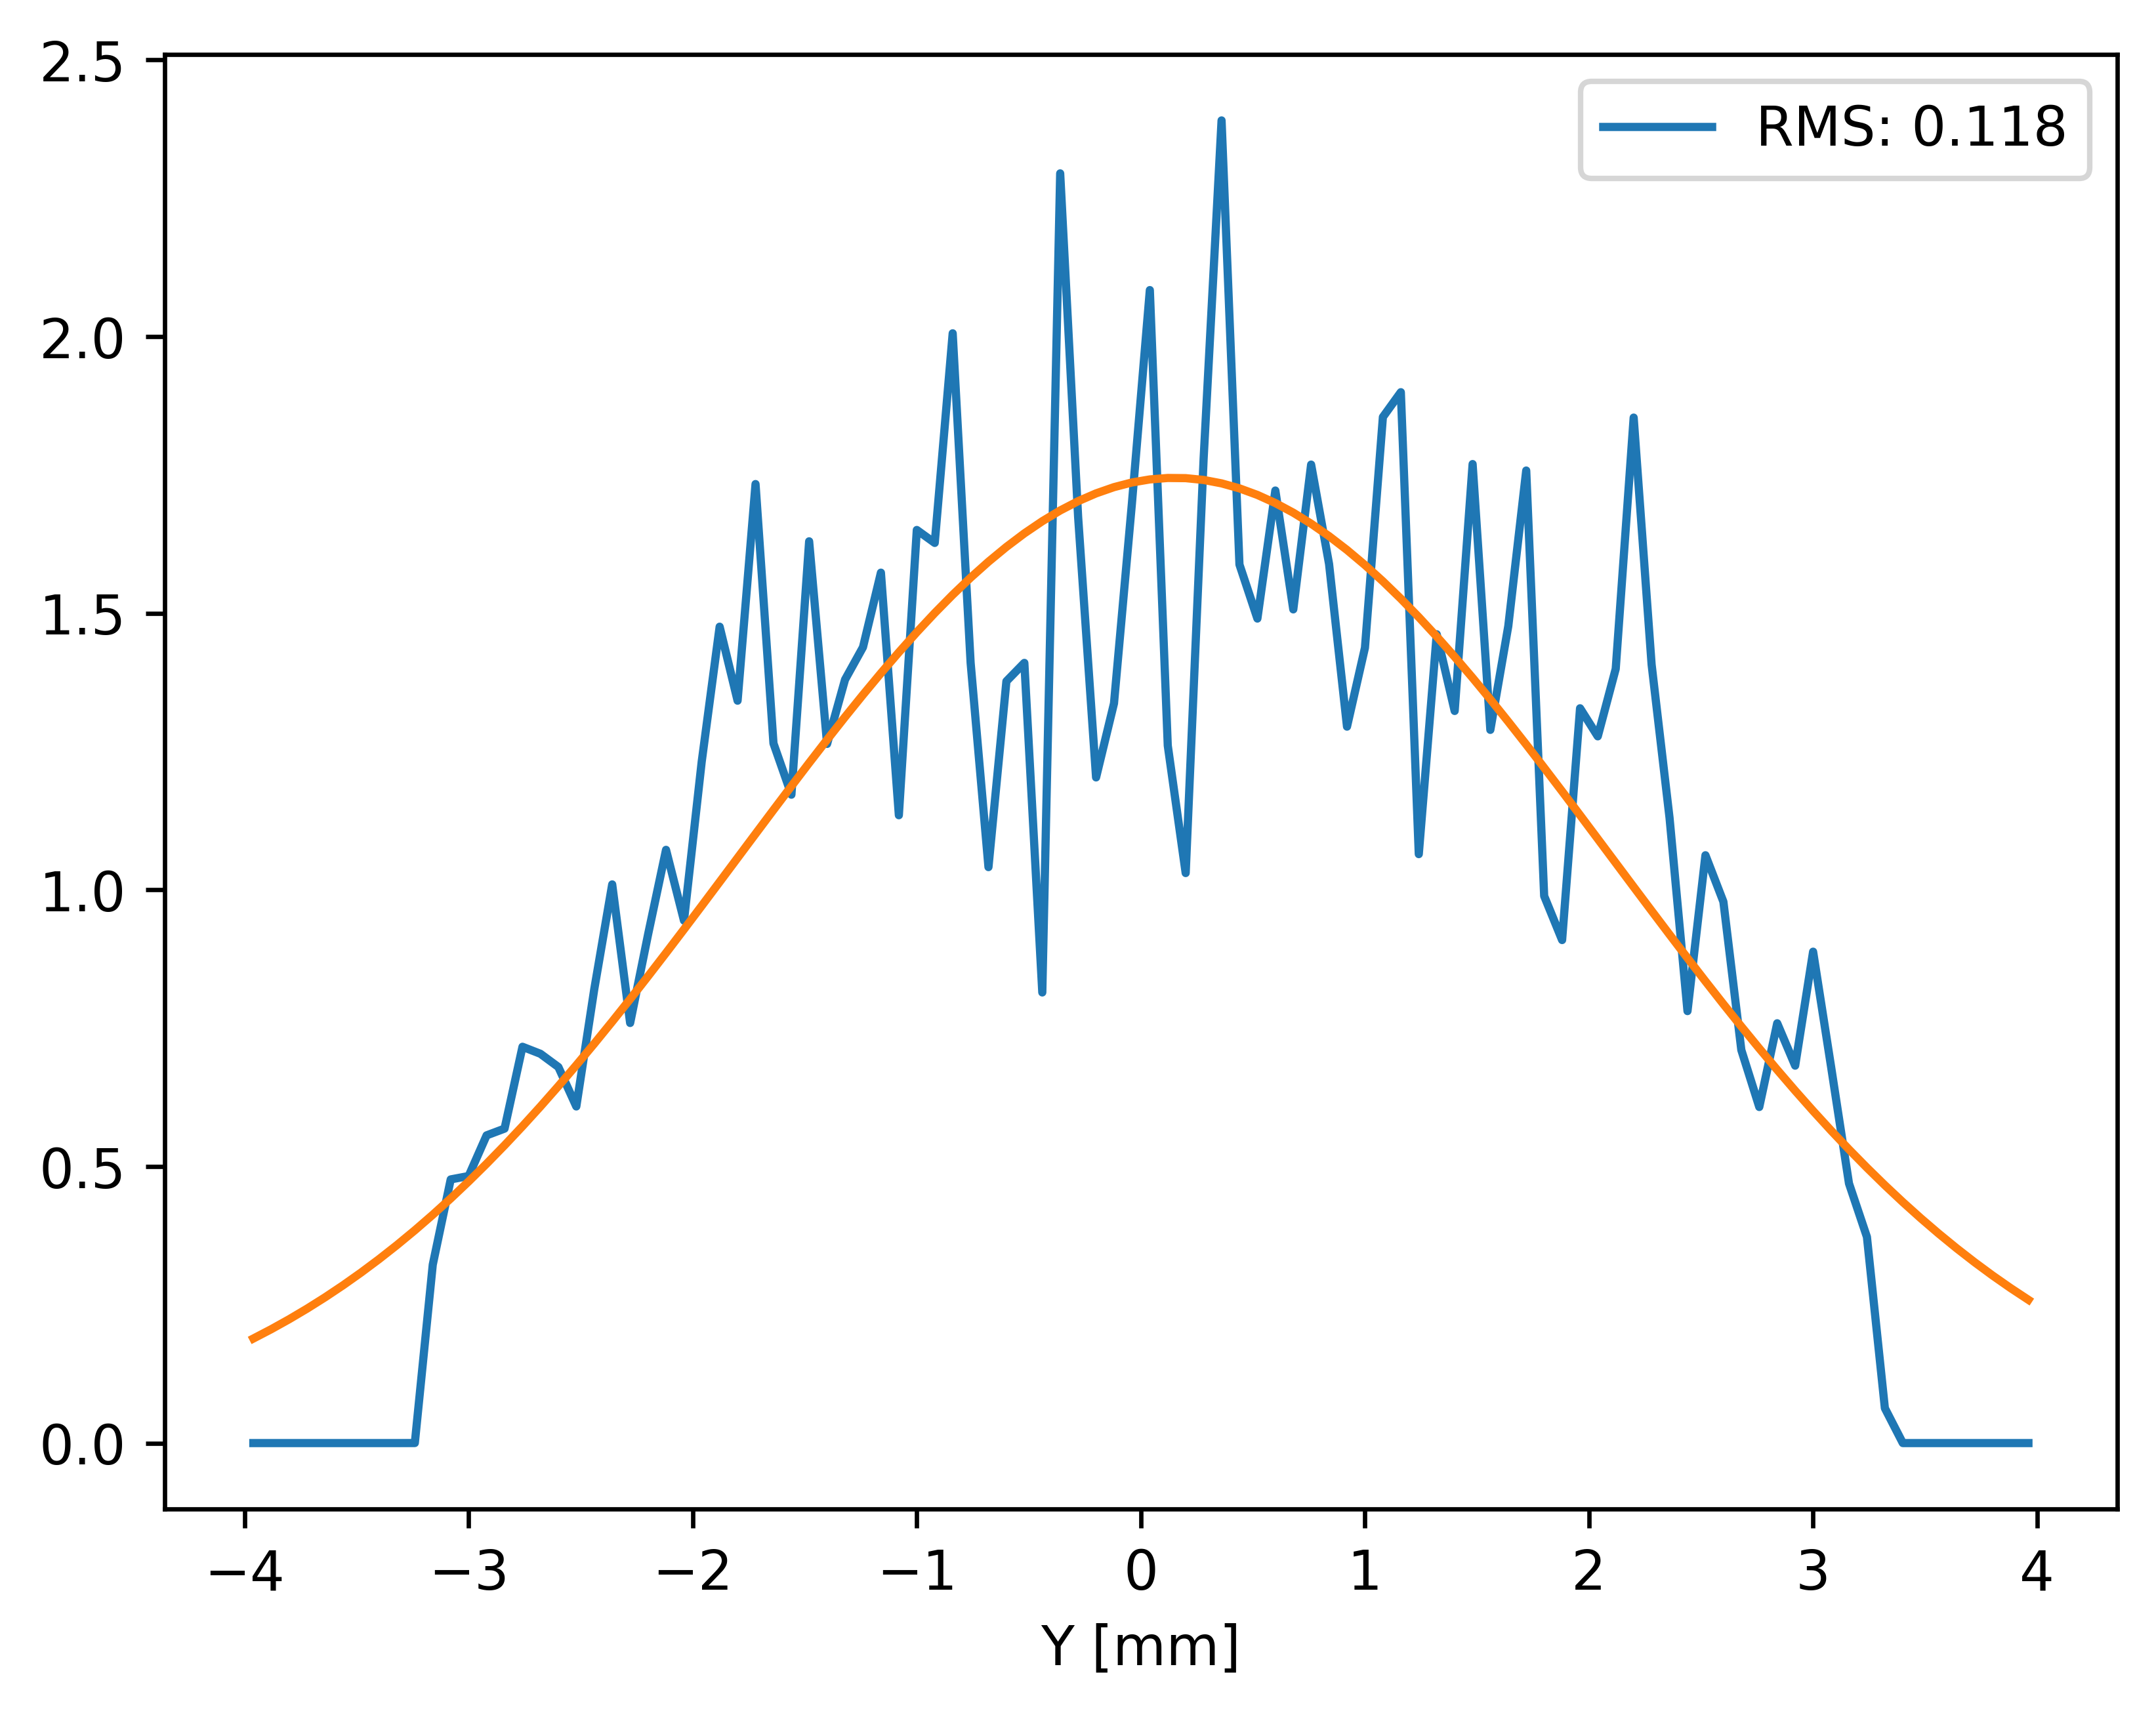
\includegraphics[width=0.9\linewidth]{./../figures/slope_error/WB4C_d30_d-spacing_gradient_45keV_slope_error03urad_Yprofile.png}
\caption{0.3 urad}
\label{fig:03urad}
\end{figure}

%%%%%%%%%%%%%%%%%%%%%%%%%%%%%%%%%%%%%%%%%%%%%%%%%%%%%%%%%%%%%%%%%%%%%%%%%%%%%%%%%%
\clearpage
\subsubsection{0.35 urad}
\begin{figure}[H]
\centering
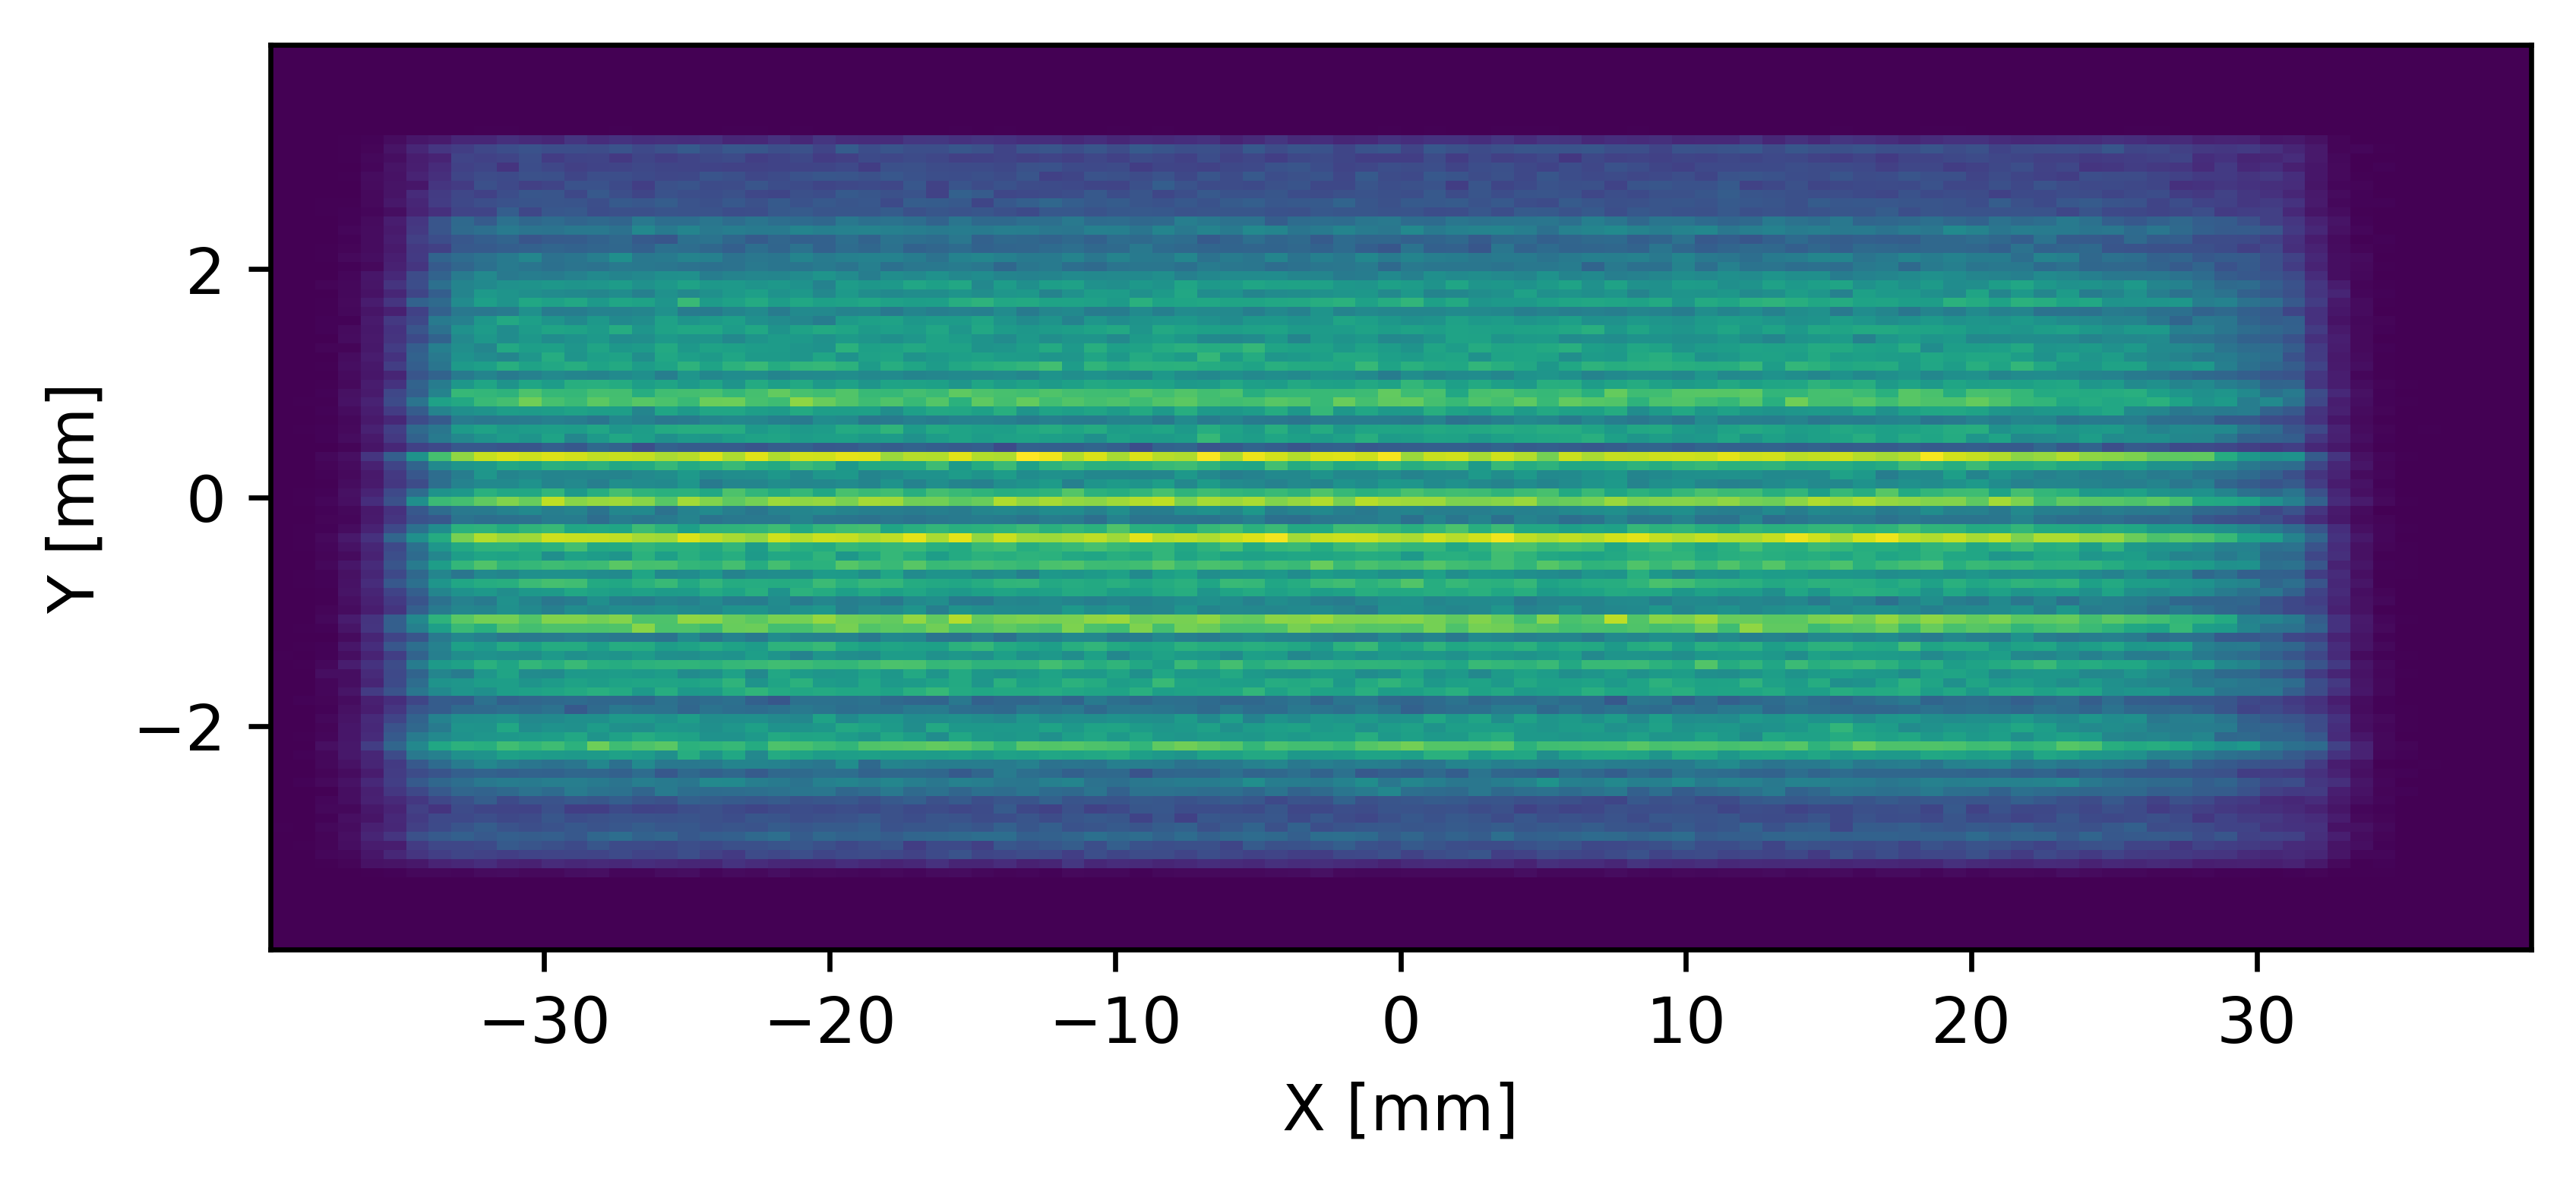
\includegraphics[width=0.9\linewidth]{./../figures/slope_error/WB4C_d30_d-spacing_gradient_45keV_slope_error035urad.png}
\end{figure}

\begin{figure}[H]
\centering
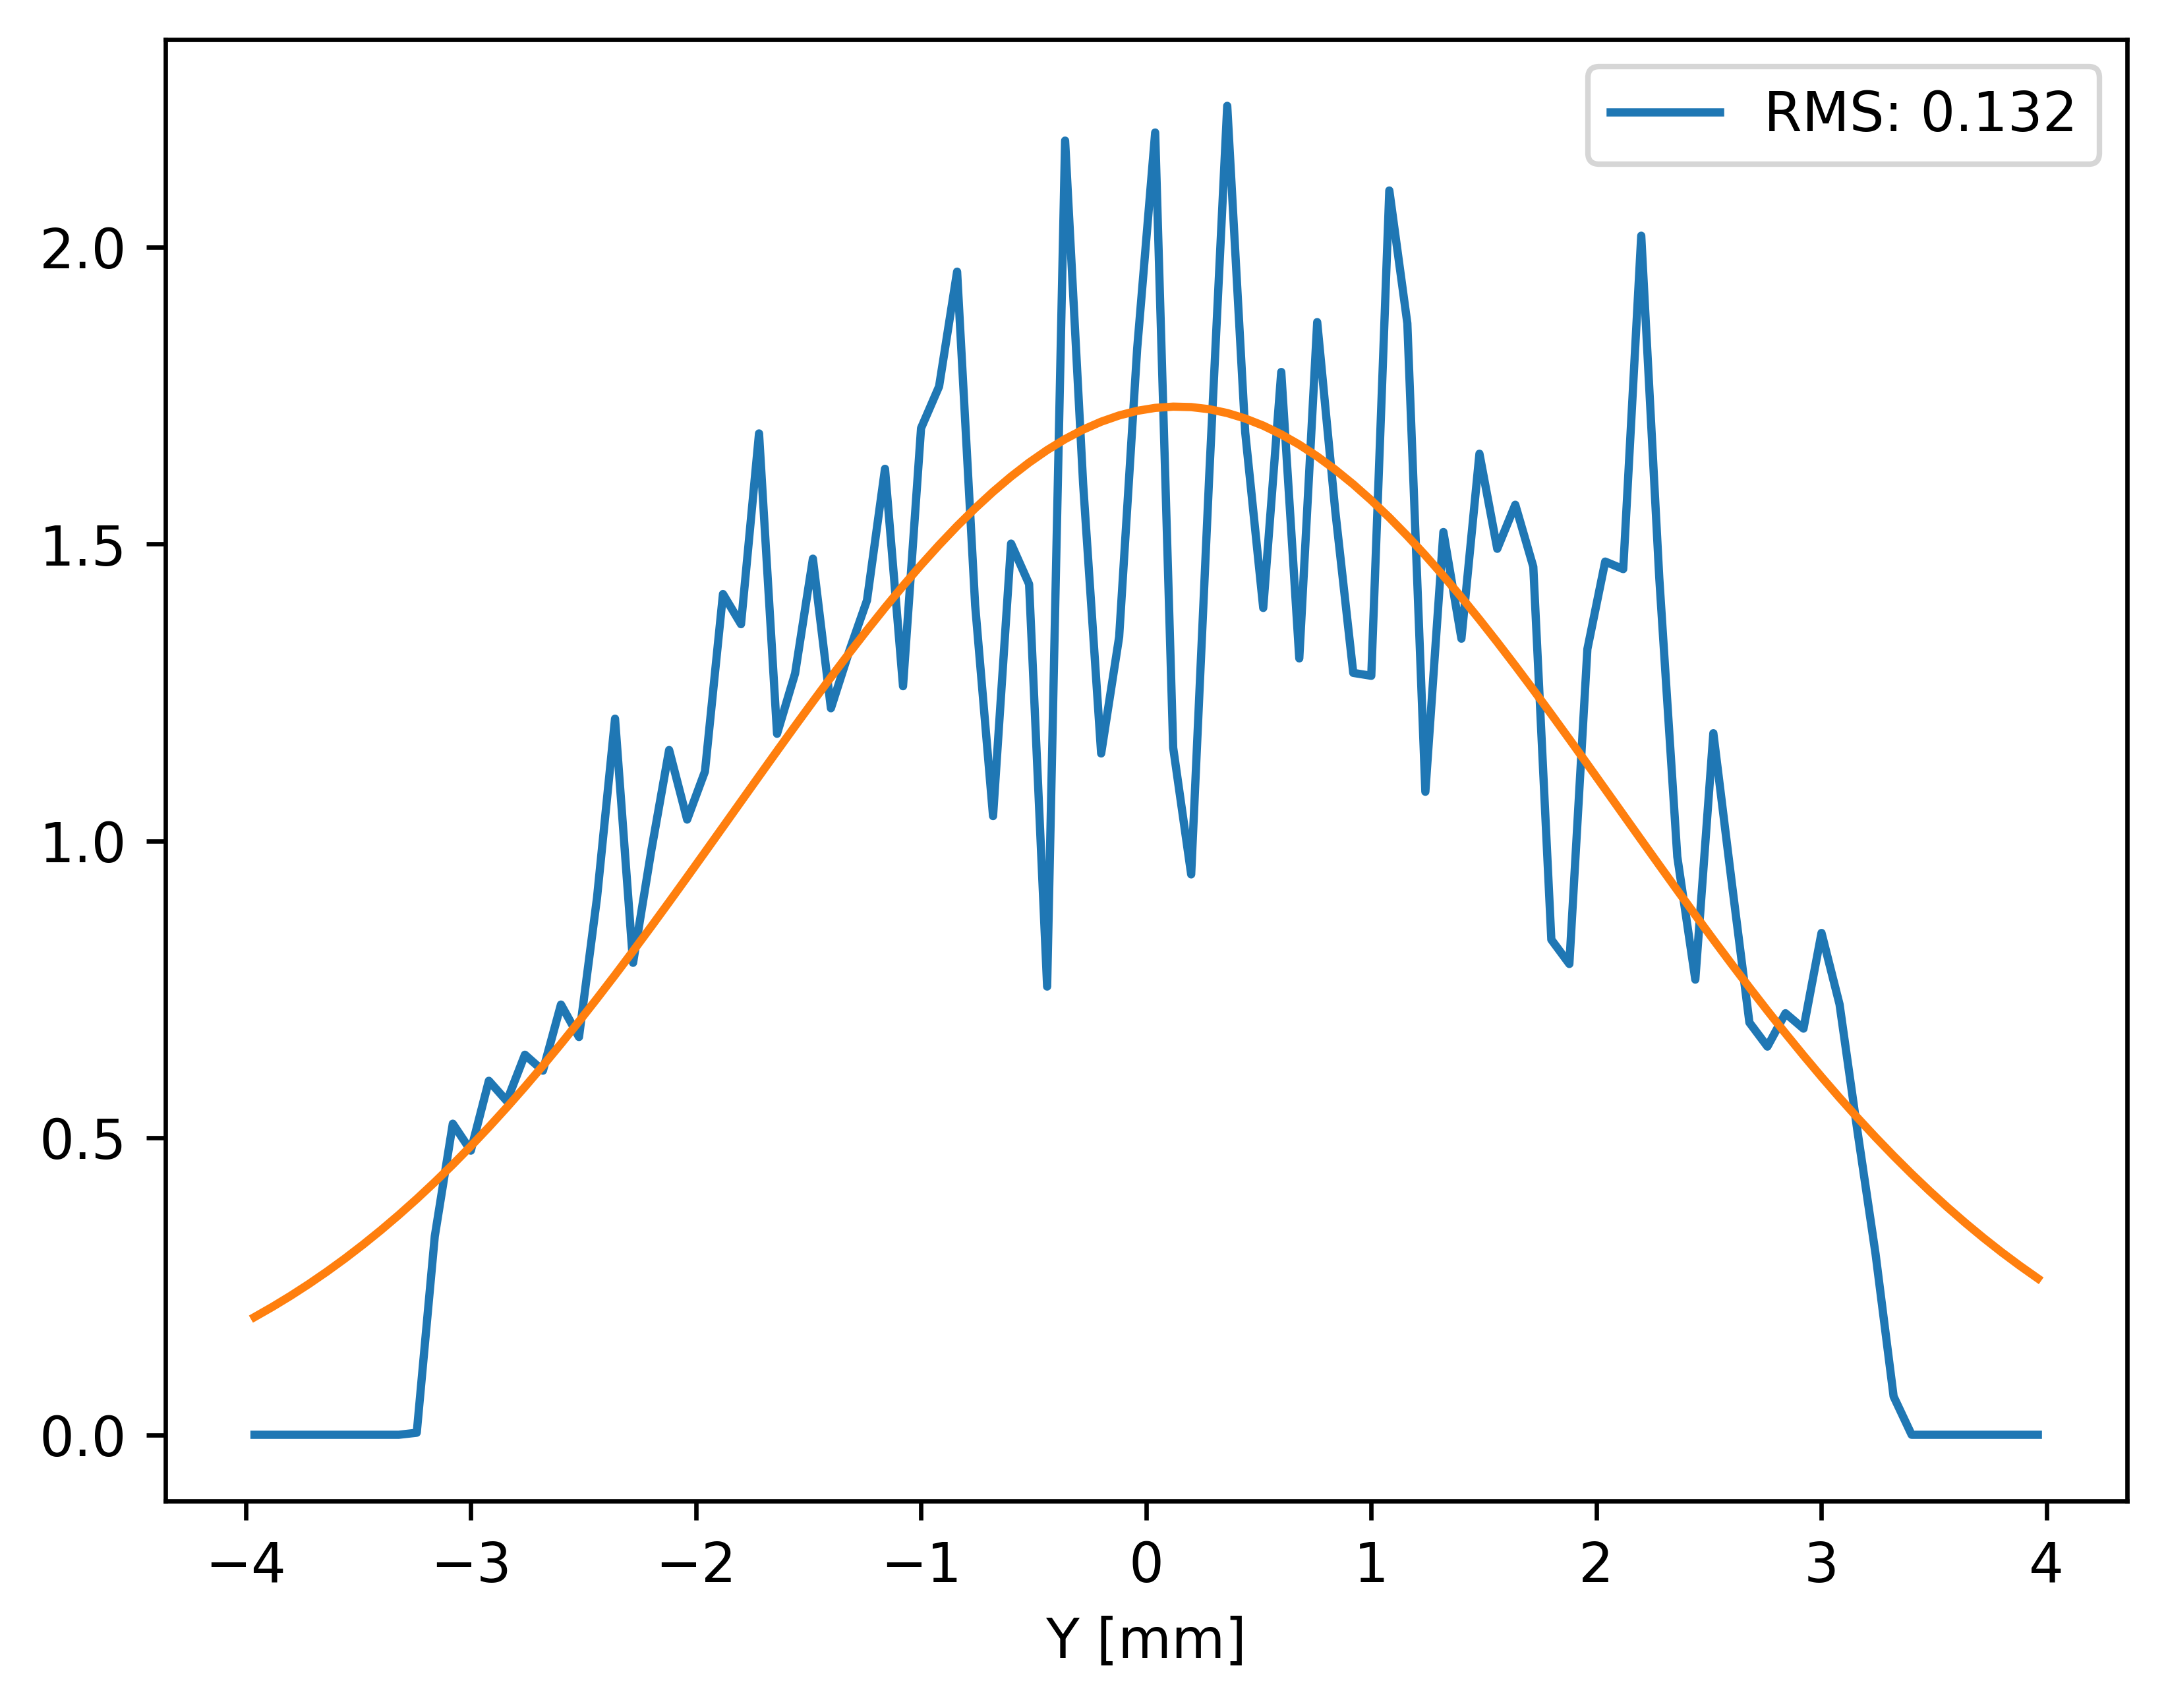
\includegraphics[width=0.9\linewidth]{./../figures/slope_error/WB4C_d30_d-spacing_gradient_45keV_slope_error035urad_Yprofile.png}
\caption{0.35 urad}
\label{fig:035urad}
\end{figure}

%%%%%%%%%%%%%%%%%%%%%%%%%%%%%%%%%%%%%%%%%%%%%%%%%%%%%%%%%%%%%%%%%%%%%%%%%%%%%%%%%%
\clearpage
\subsubsection{0.4 urad}
\begin{figure}[H]
\centering
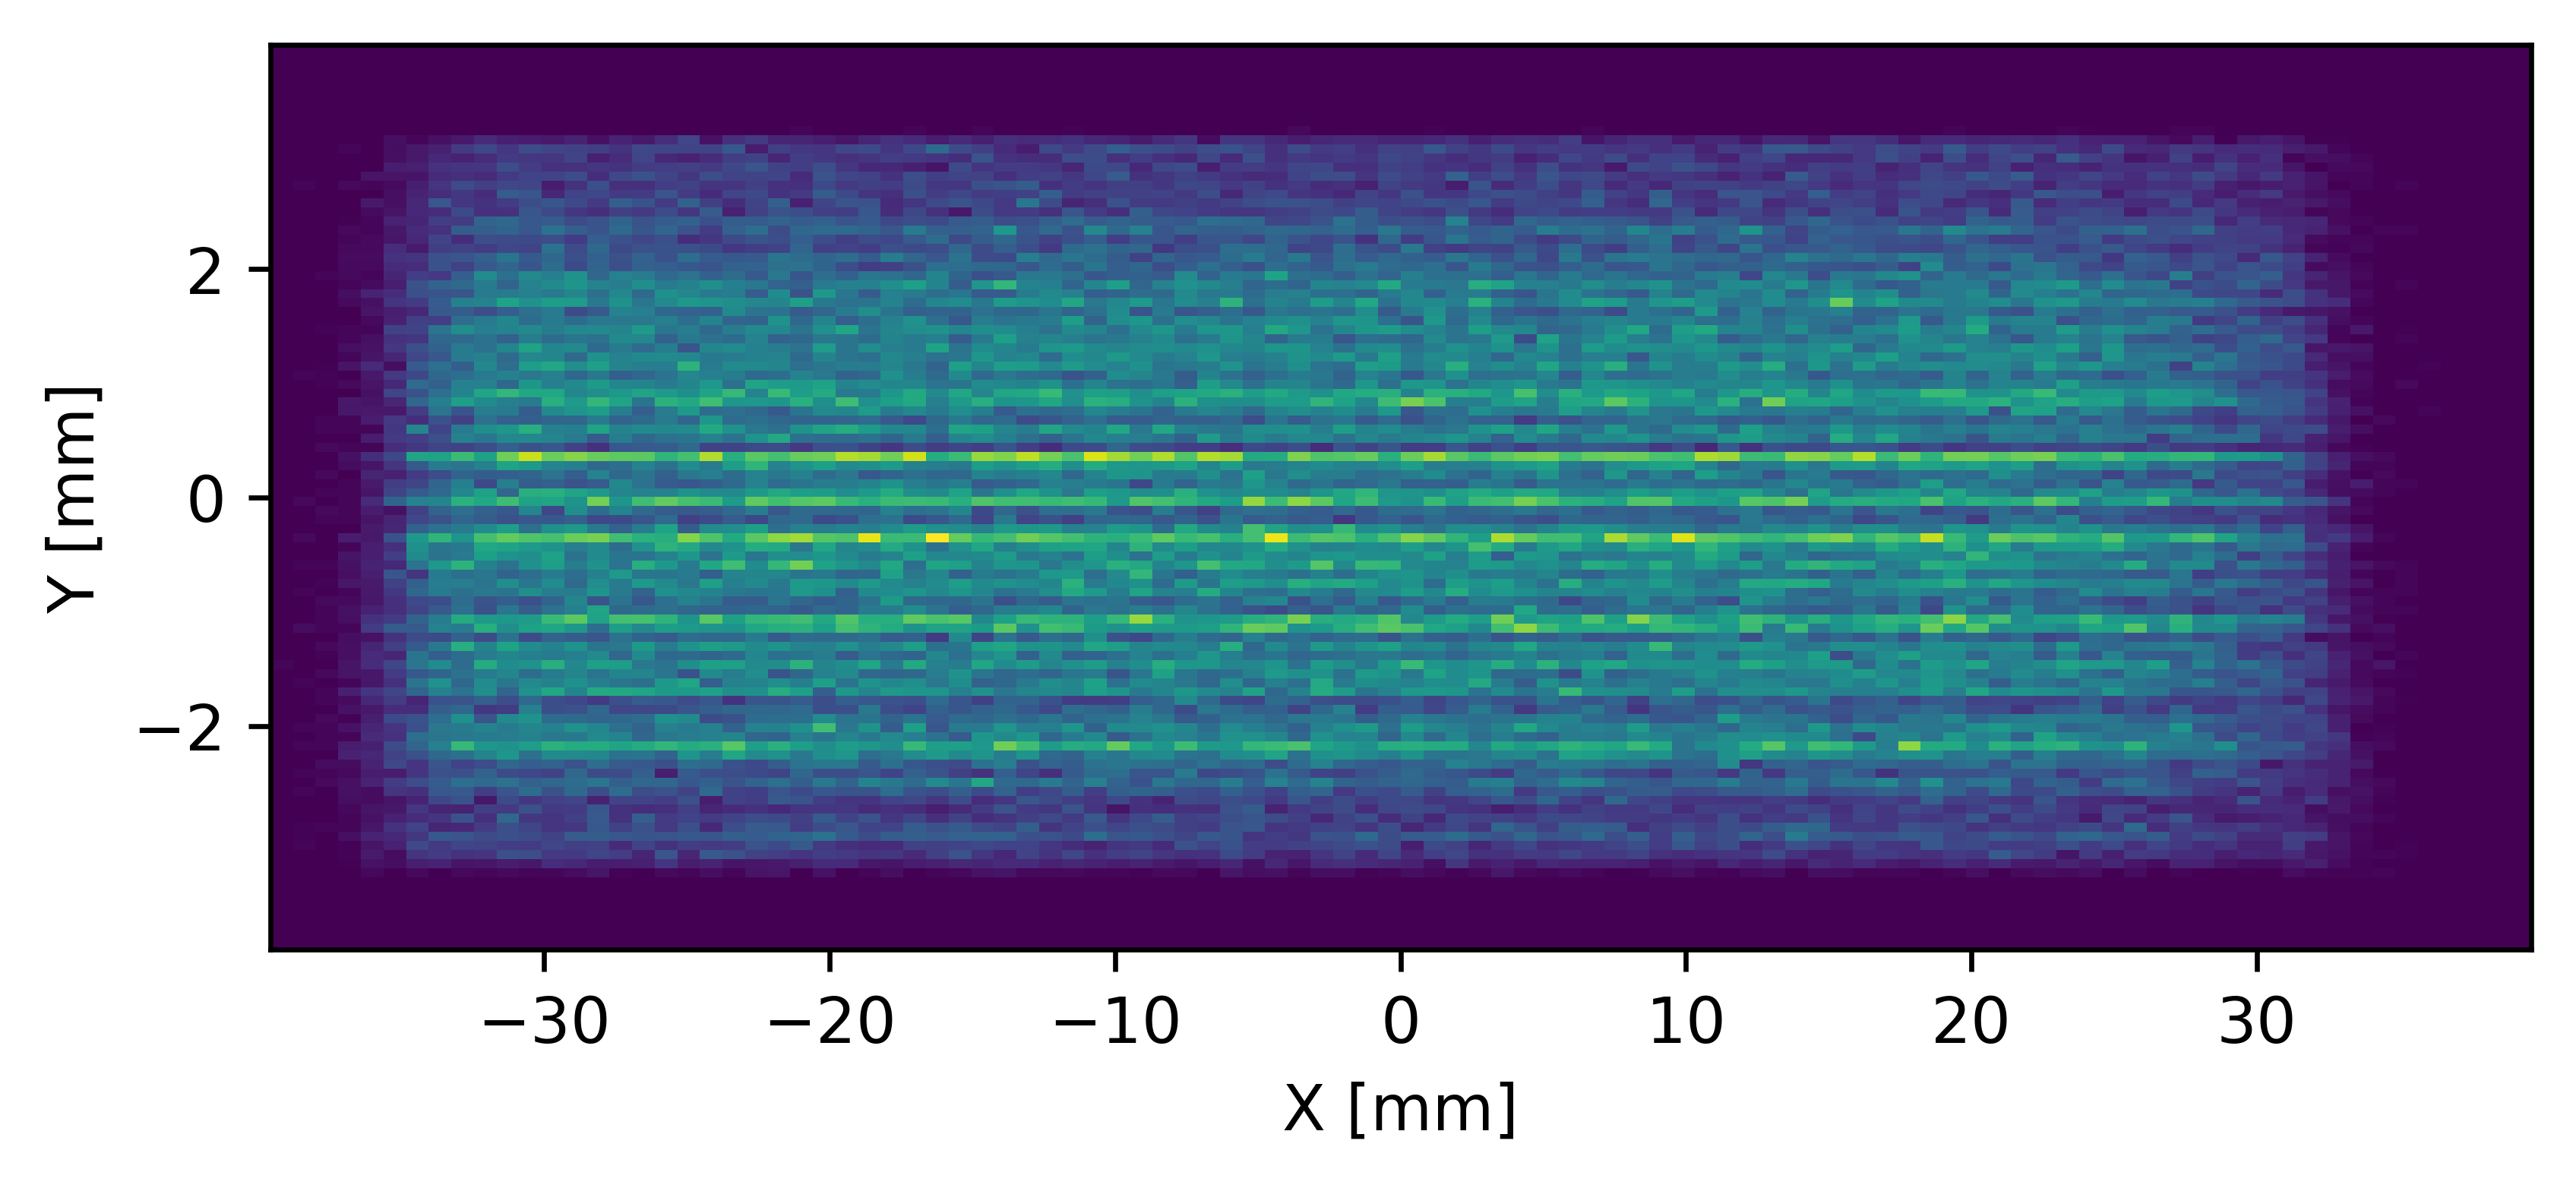
\includegraphics[width=0.9\linewidth]{./../figures/slope_error/WB4C_d30_d-spacing_gradient_45keV_slope_error04urad.png}
\end{figure}

\begin{figure}[H]
\centering
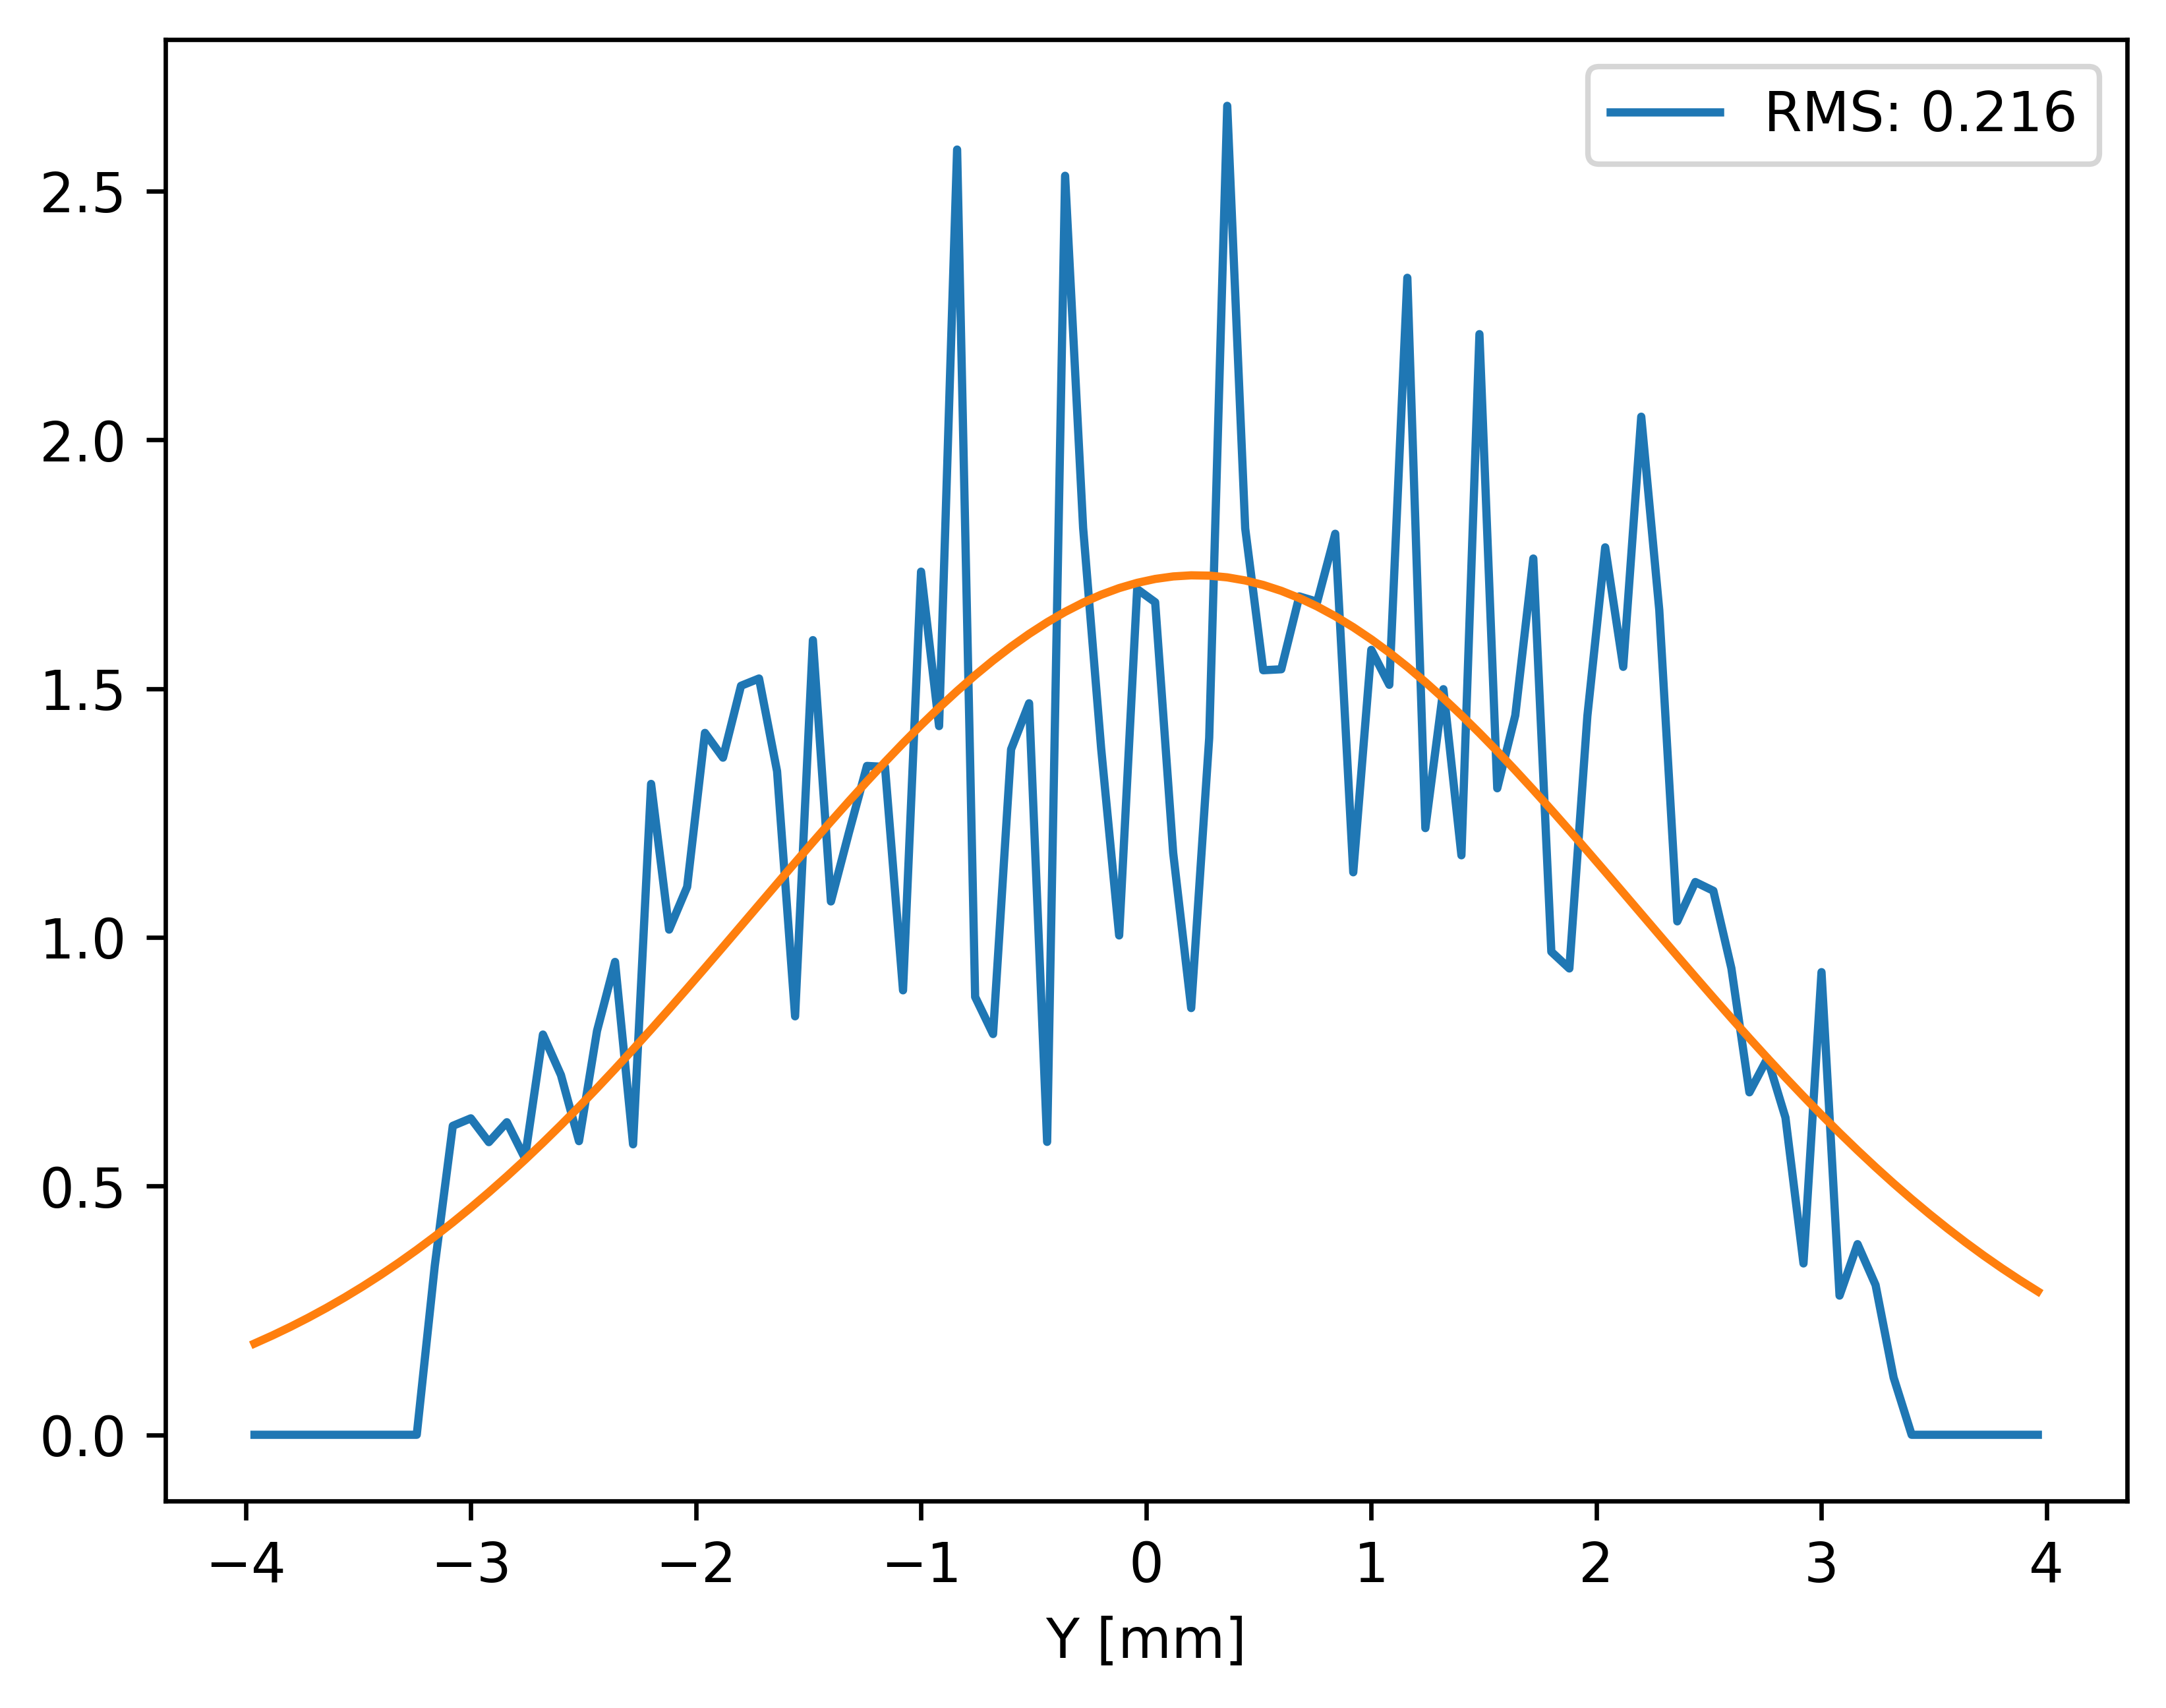
\includegraphics[width=0.9\linewidth]{./../figures/slope_error/WB4C_d30_d-spacing_gradient_45keV_slope_error04urad_Yprofile.png}
\caption{0.4 urad}
\label{fig:04urad}
\end{figure}

%%%%%%%%%%%%%%%%%%%%%%%%%%%%%%%%%%%%%%%%%%%%%%%%%%%%%%%%%%%%%%%%%%%%%%%%%%%%%%%%%%
\clearpage
\subsubsection{0.5 urad}
\begin{figure}[H]
\centering
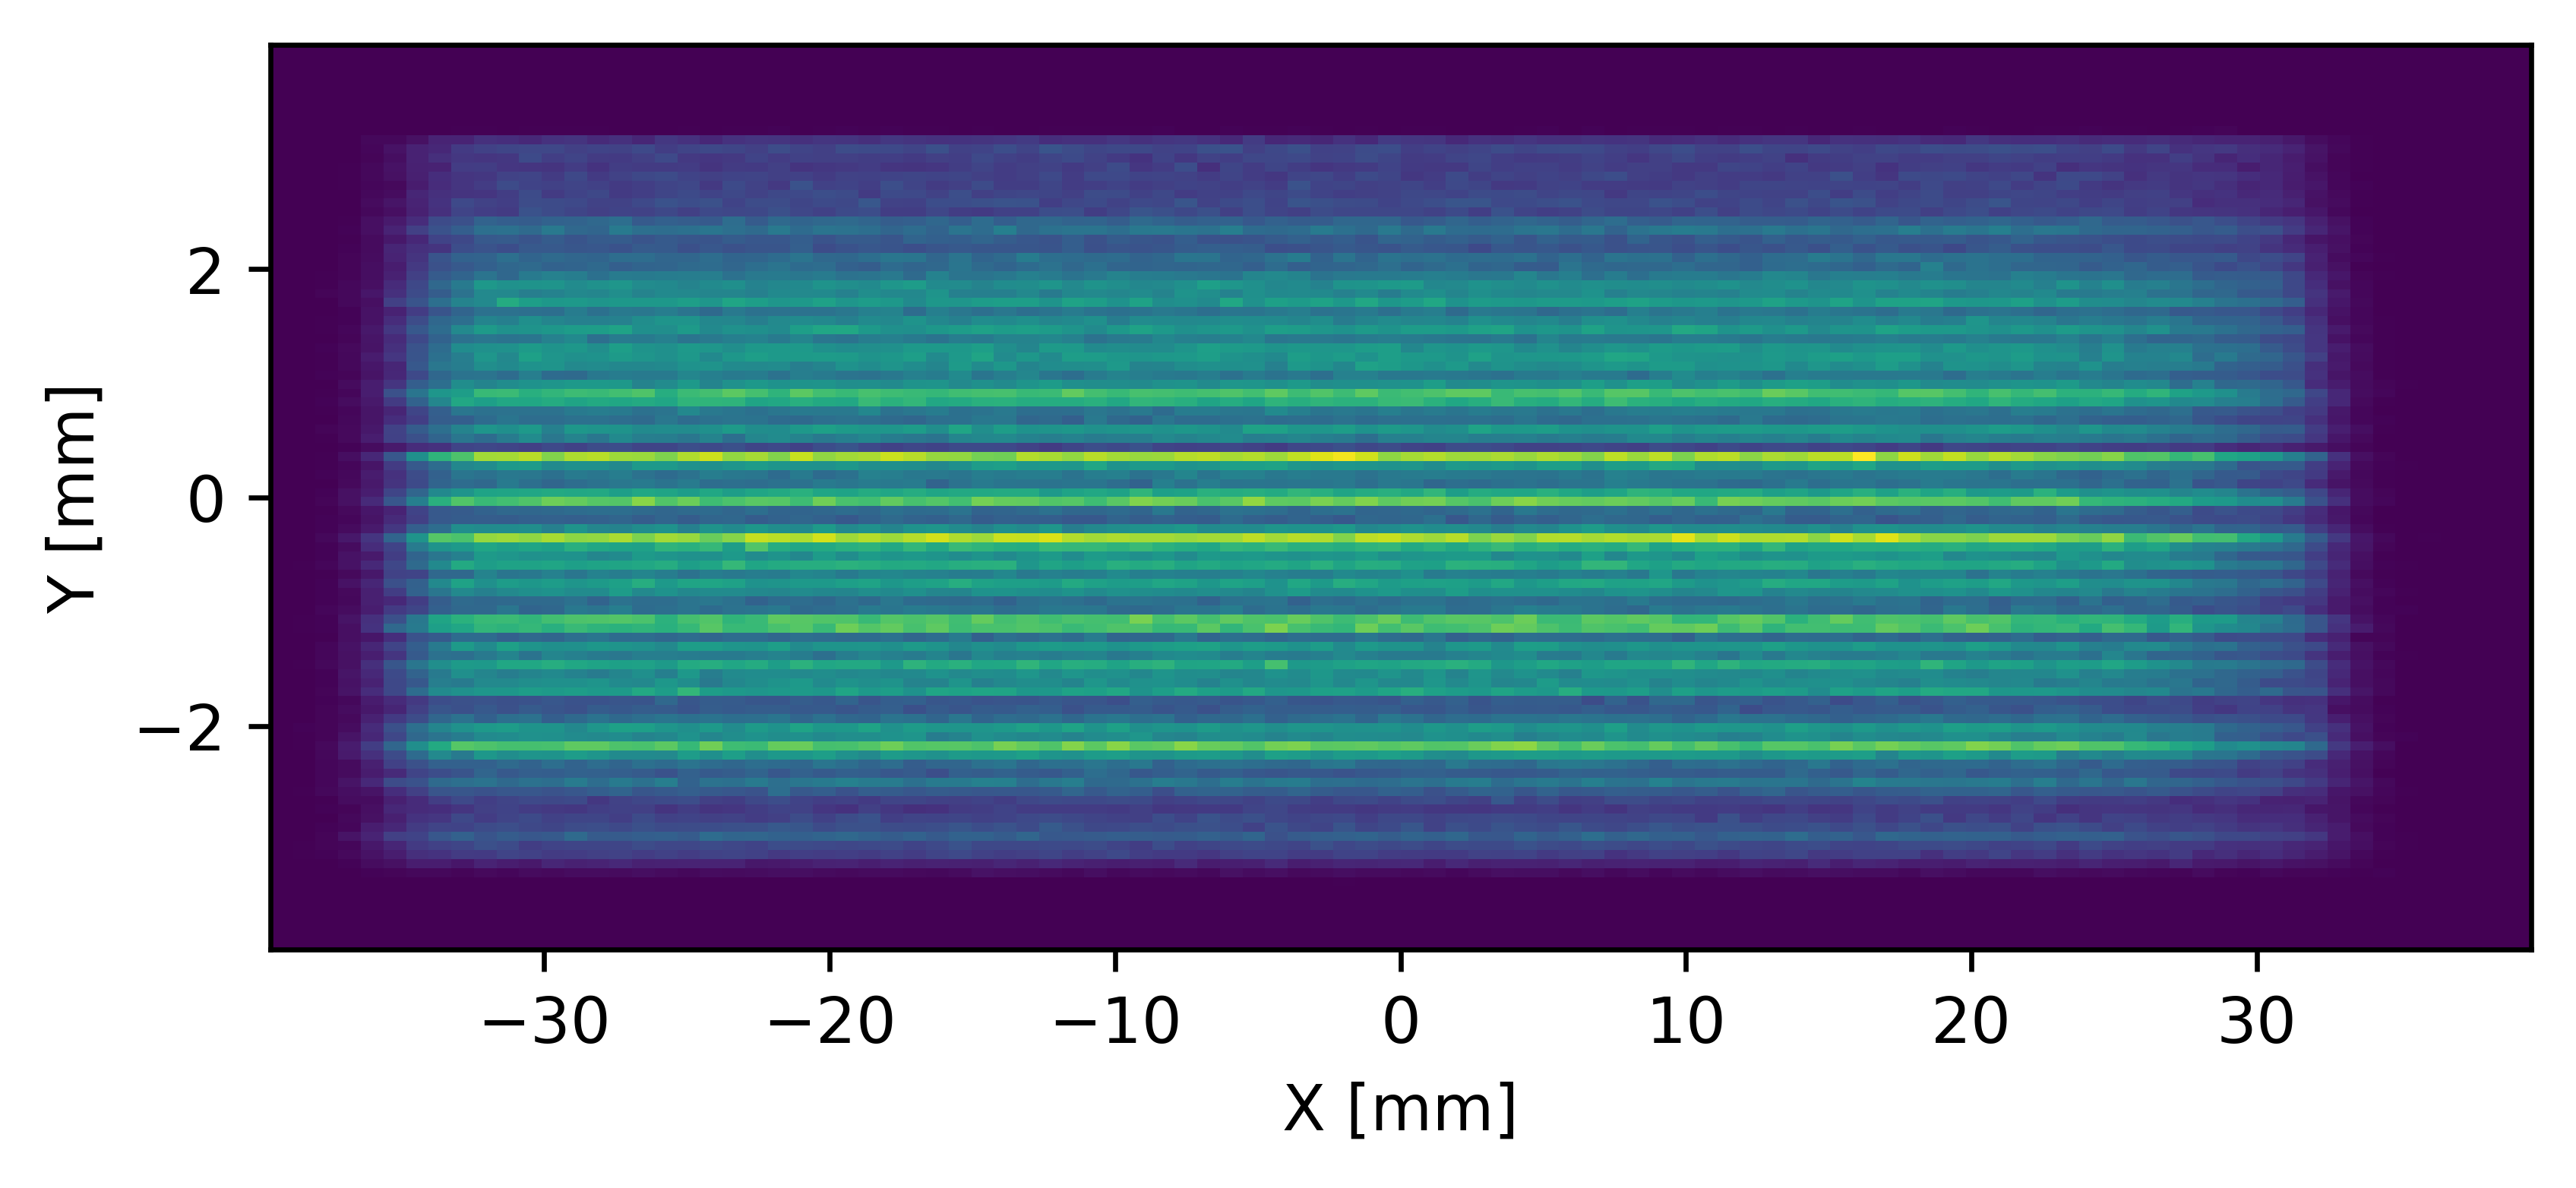
\includegraphics[width=0.9\linewidth]{./../figures/slope_error/WB4C_d30_d-spacing_gradient_45keV_slope_error05urad.png}
\end{figure}

\begin{figure}[H]
\centering
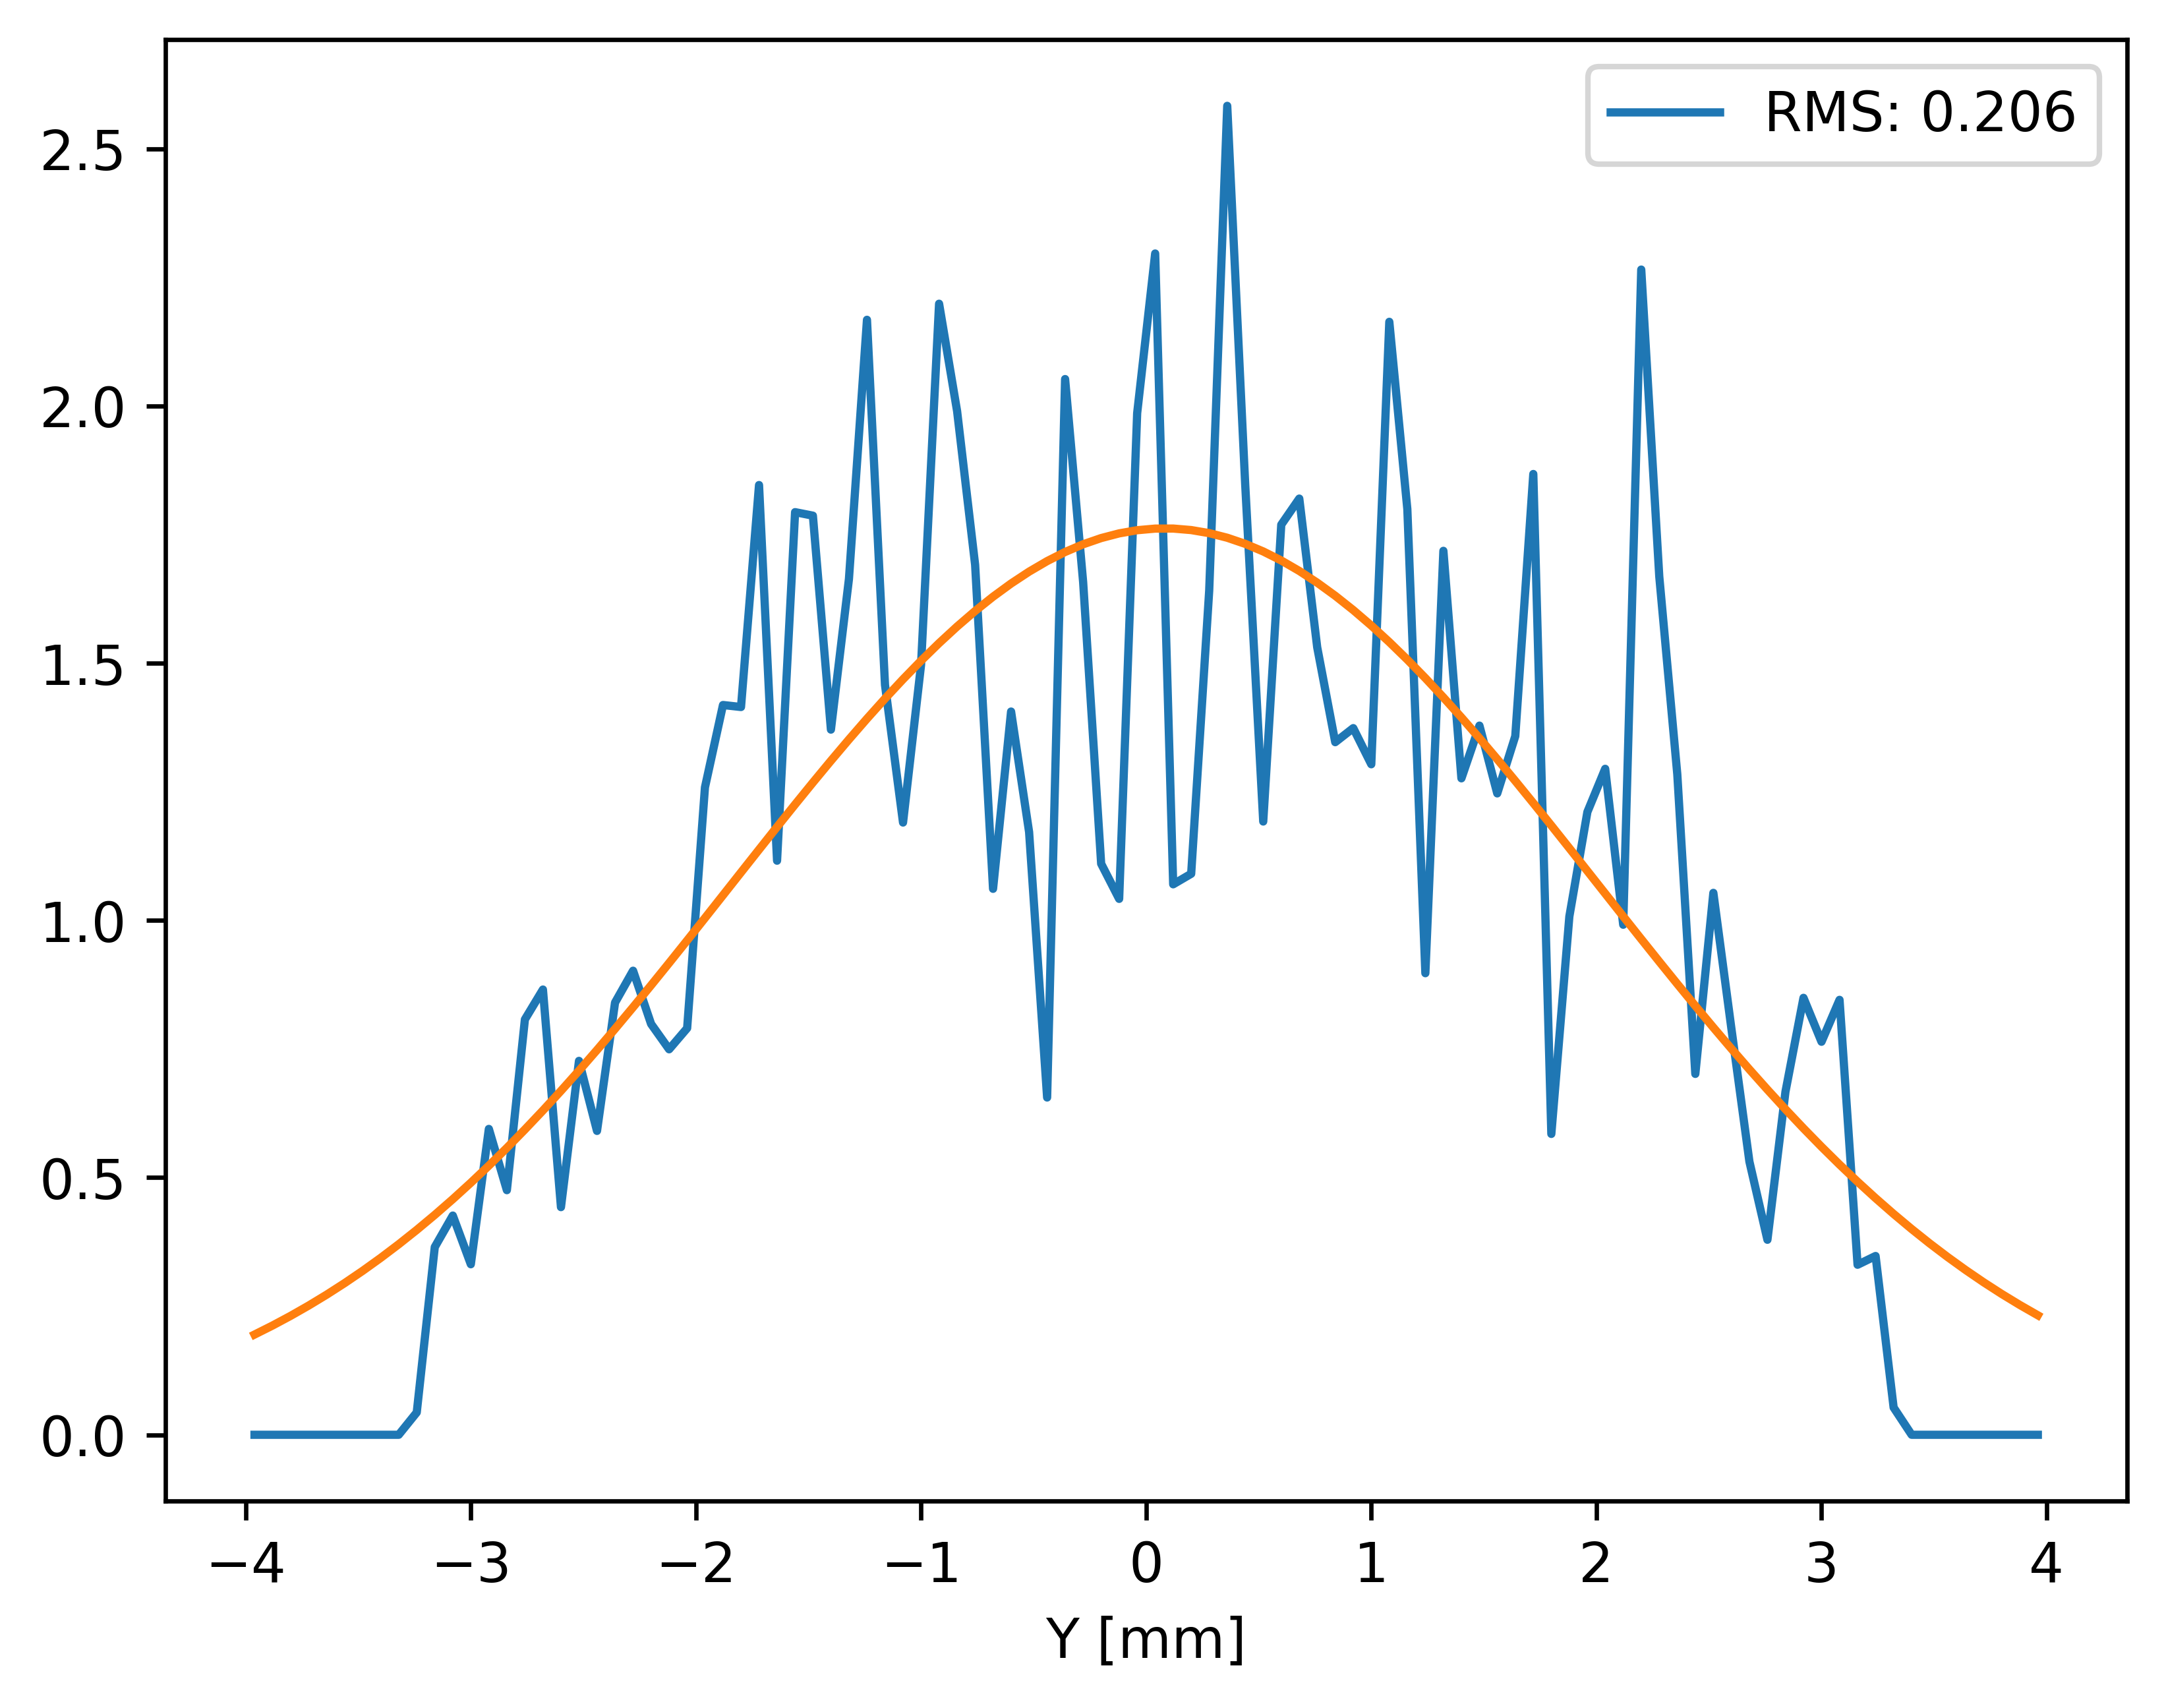
\includegraphics[width=0.9\linewidth]{./../figures/slope_error/WB4C_d30_d-spacing_gradient_45keV_slope_error05urad_Yprofile.png}
\caption{0.5 urad}
\label{fig:05urad}
\end{figure}

% \clearpage
% \subsection{Mirror slope error - ESRF ID19 source}
The ESRF ID19 PW150 source is considered for this paragraph for comparison. All remaining BL and mirror components are identical. 

\subsubsection{0.1 urad}
\begin{figure}[H]
\centering
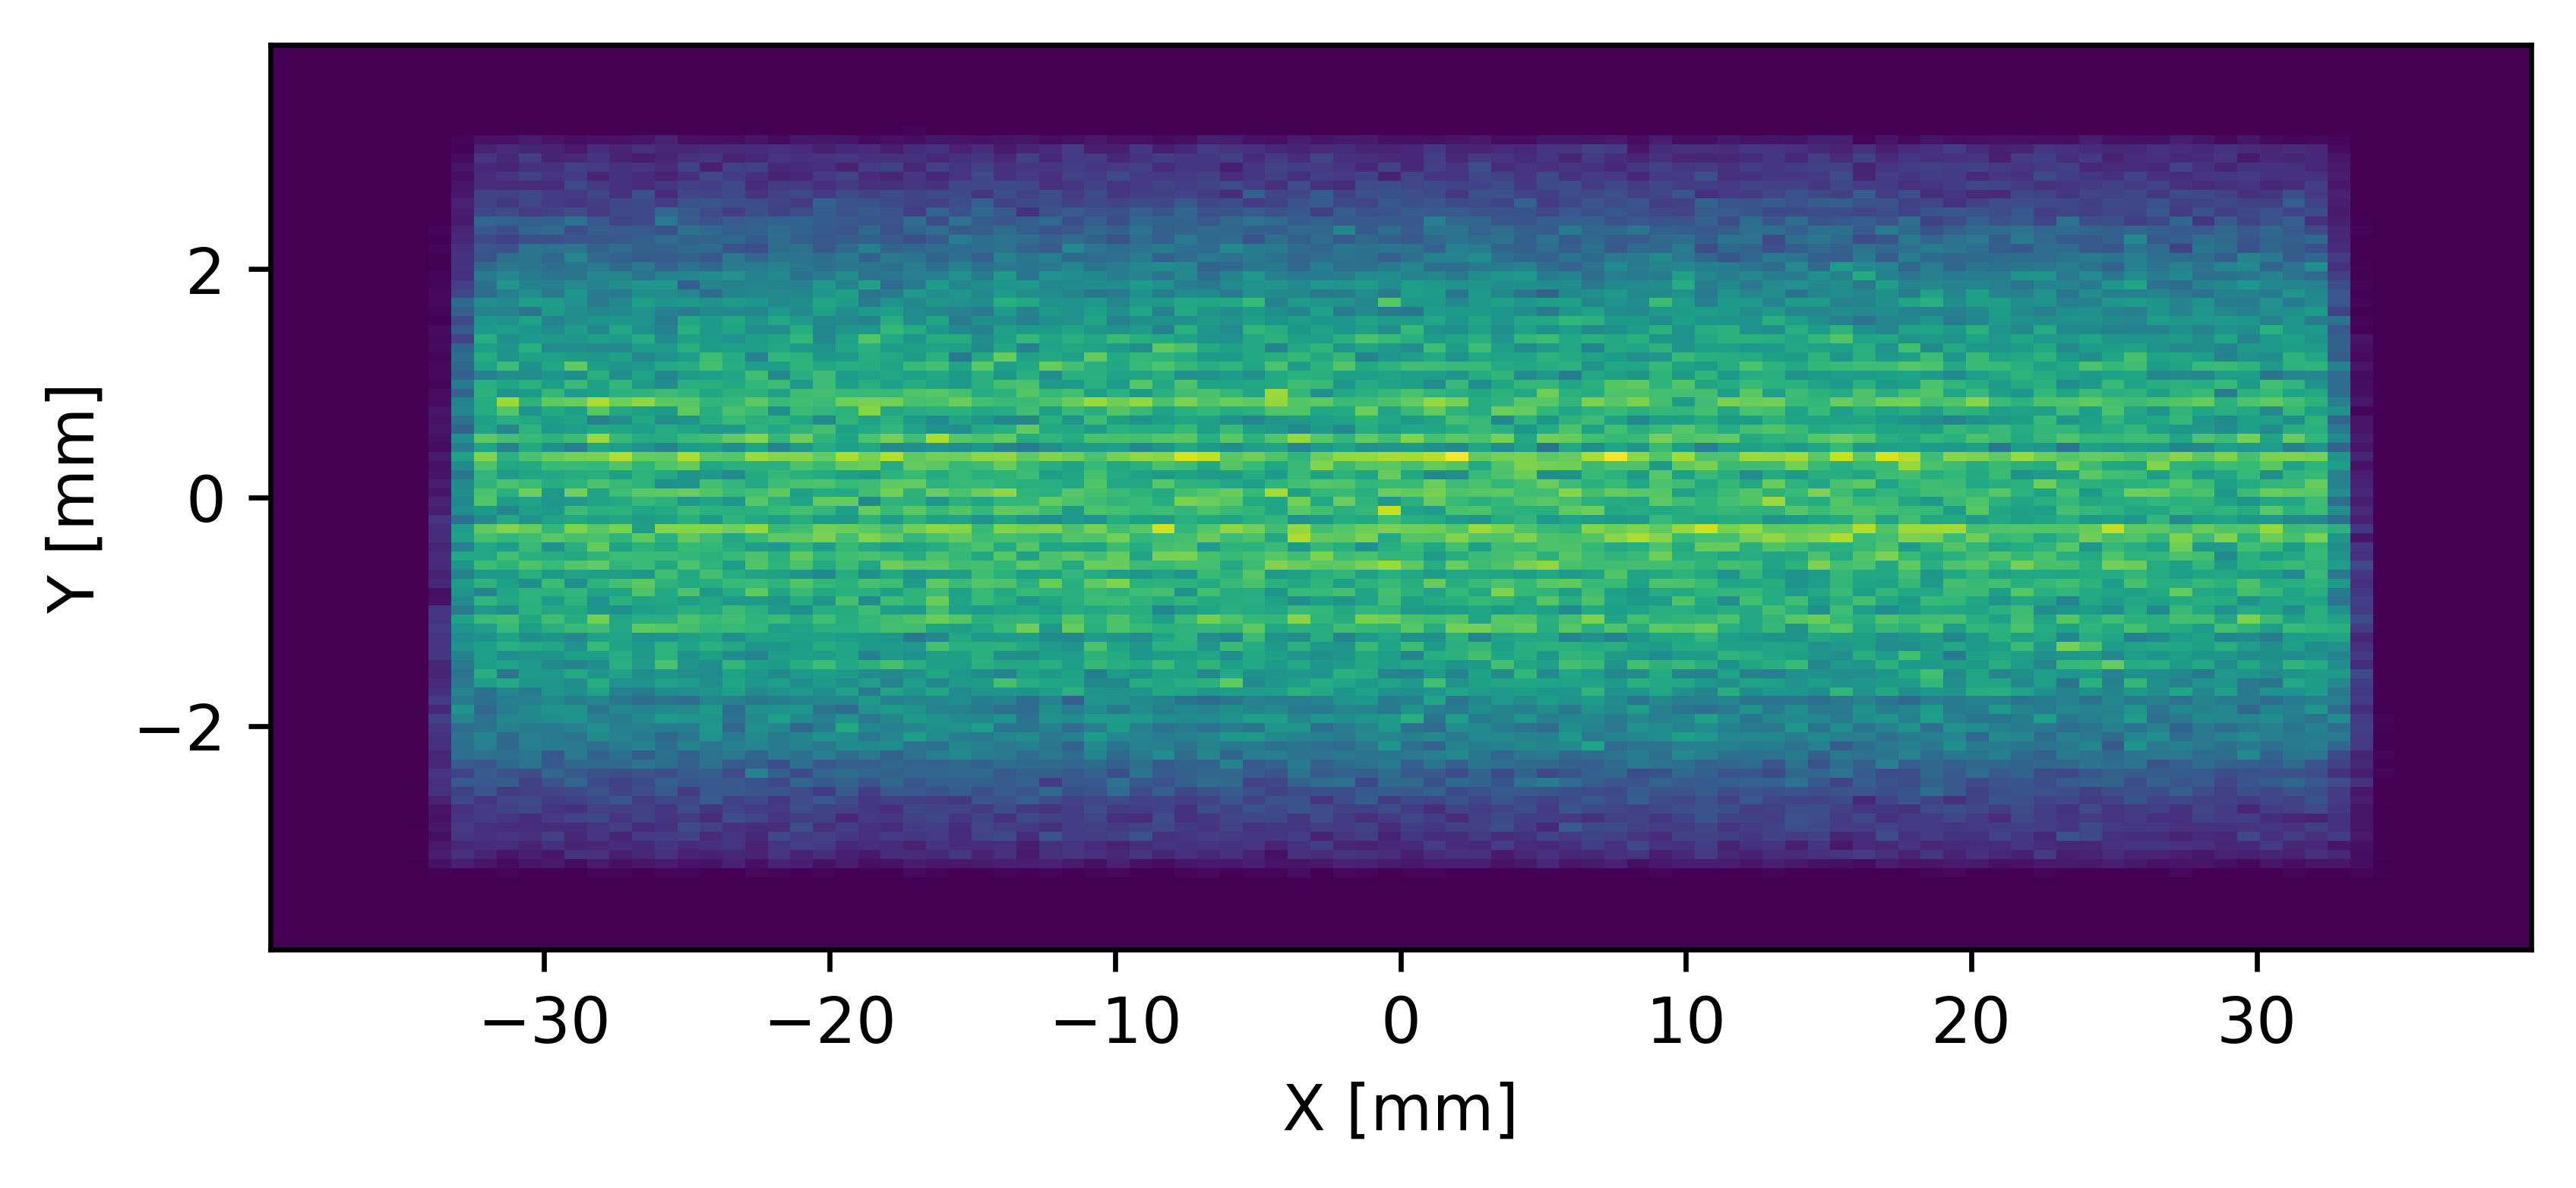
\includegraphics[width=0.85\linewidth]{./../figures/slope_error/WB4C_d30_d-spacing_gradient_45keV_slope_error01urad_ESRFID19PW150.png}
\end{figure}

\begin{figure}[H]
\centering
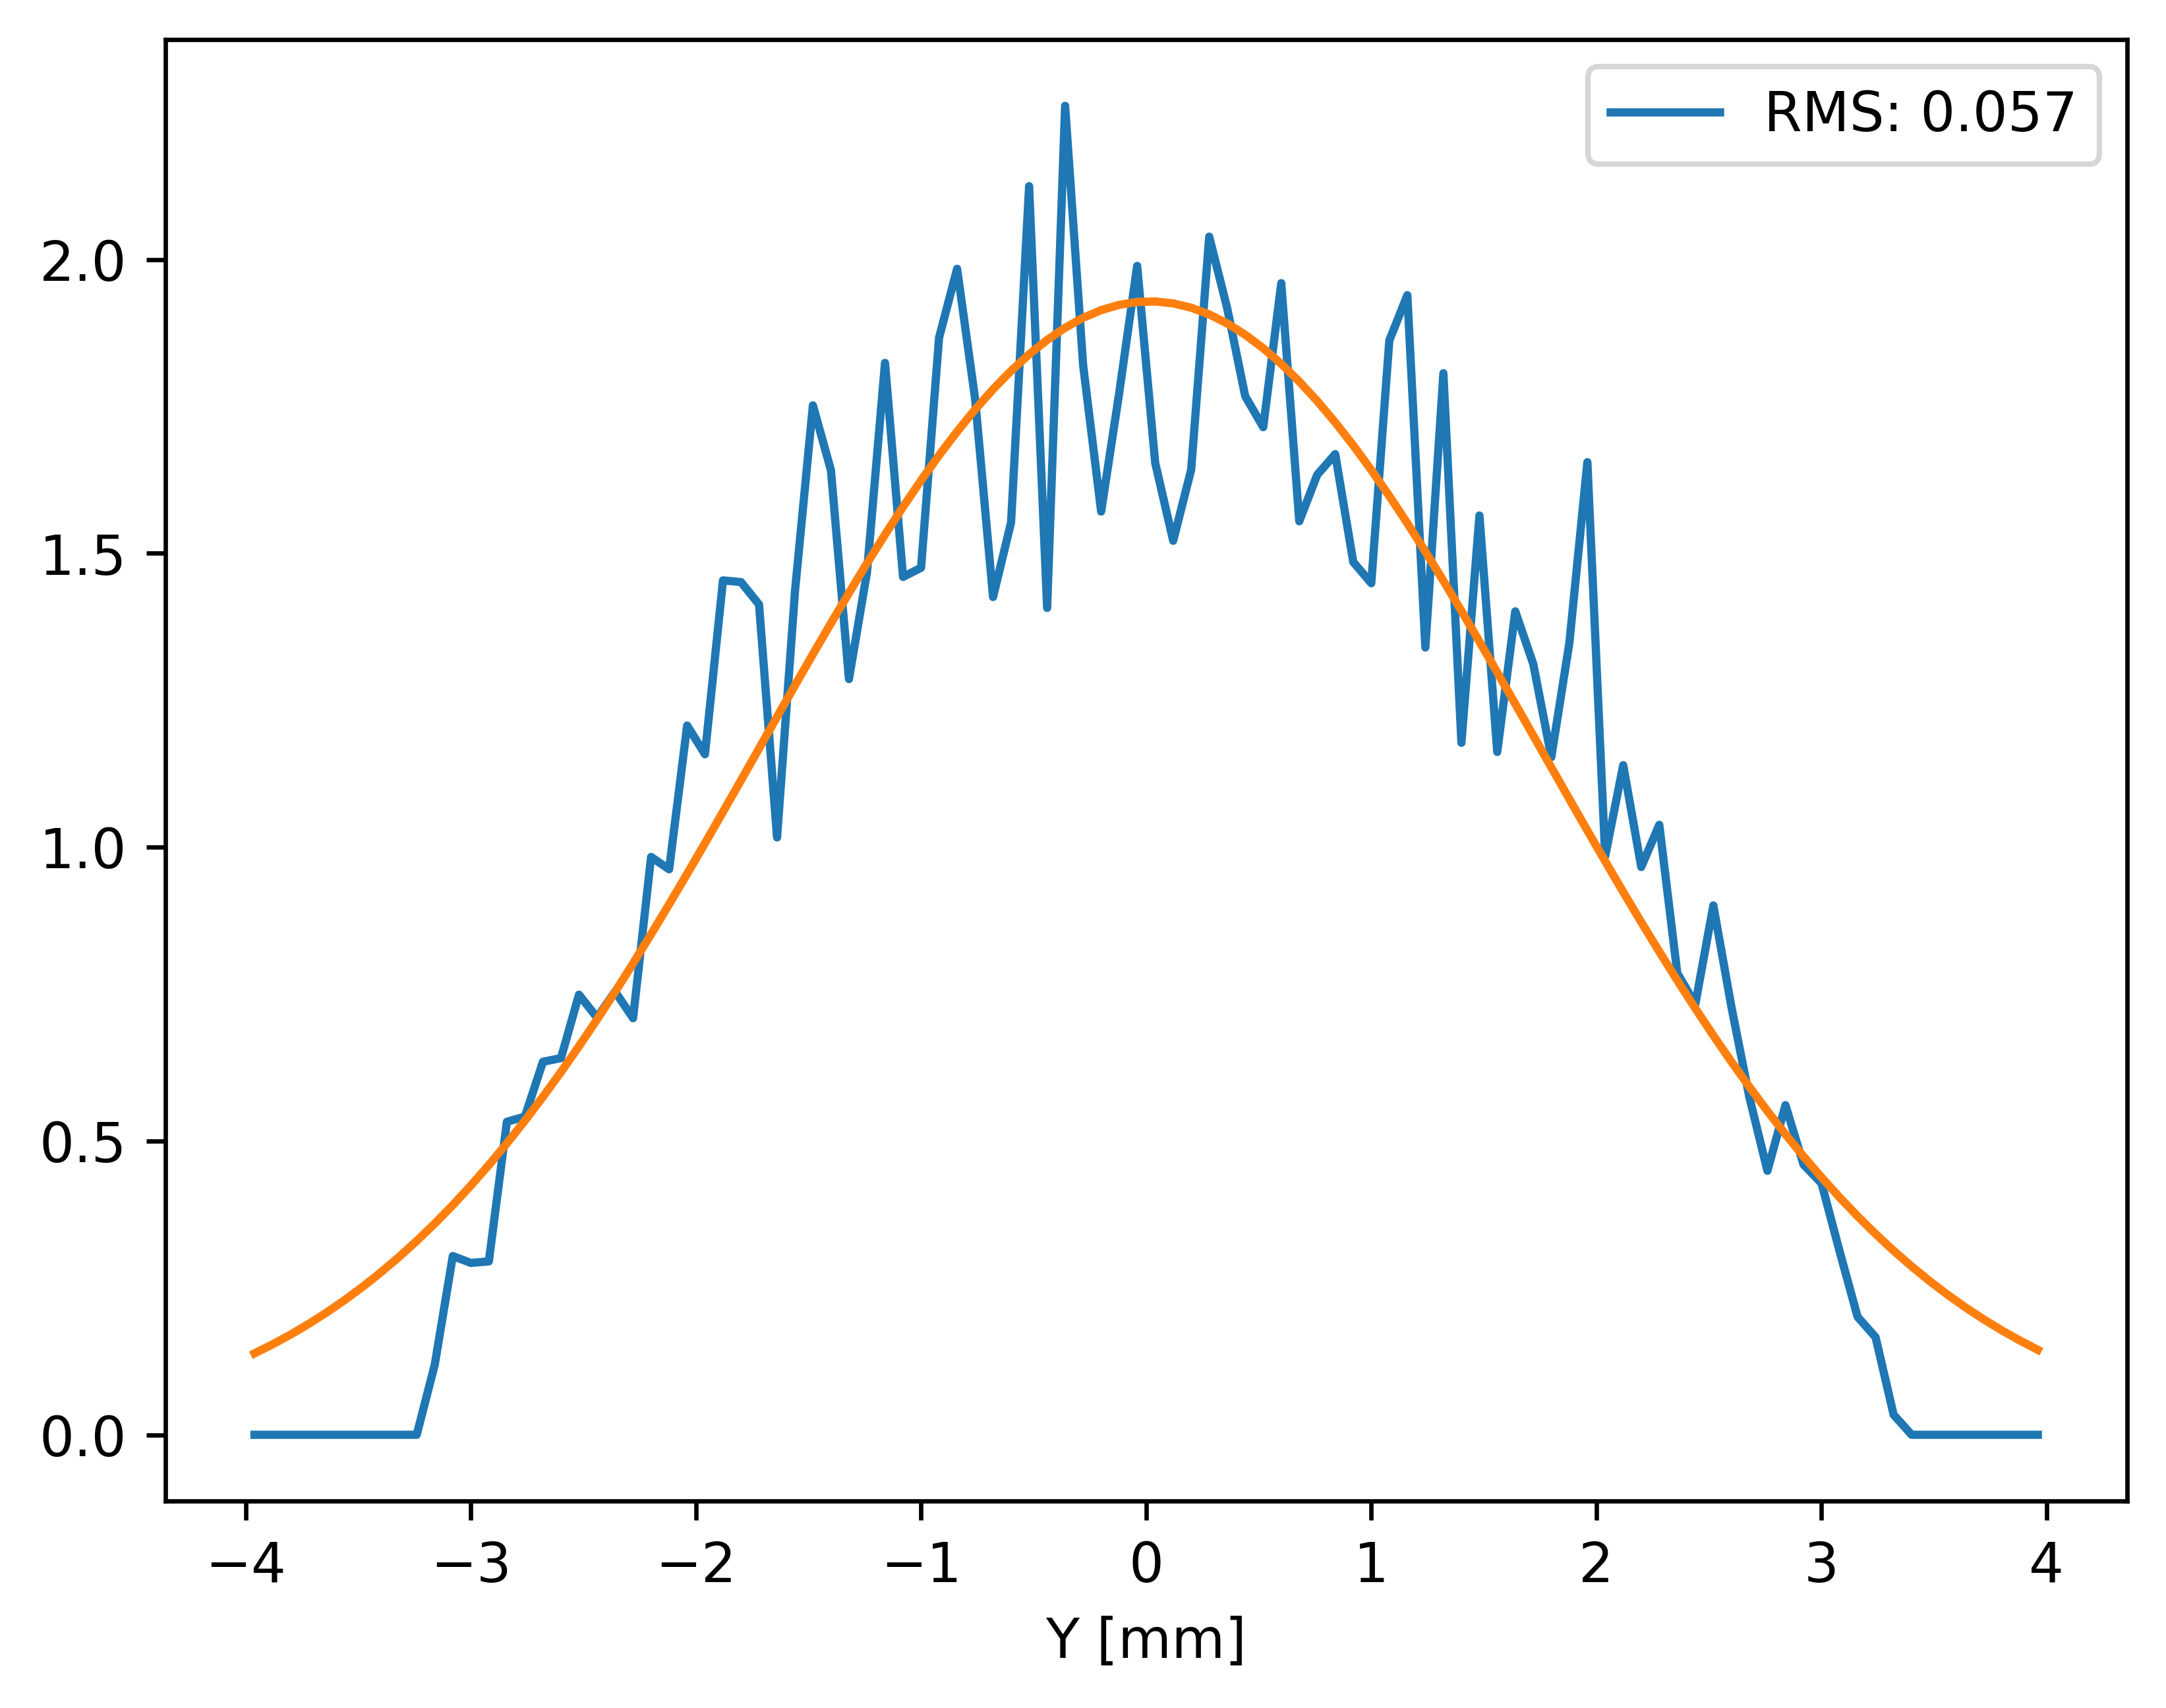
\includegraphics[width=0.85\linewidth]{./../figures/slope_error/WB4C_d30_d-spacing_gradient_45keV_slope_error01urad_ESRFID19PW150_Yprofile.png}
\caption{0.1 urad}
\label{fig:01urad}
\end{figure}

\clearpage
\subsubsection{0.2 urad}
\begin{figure}[H]
\centering
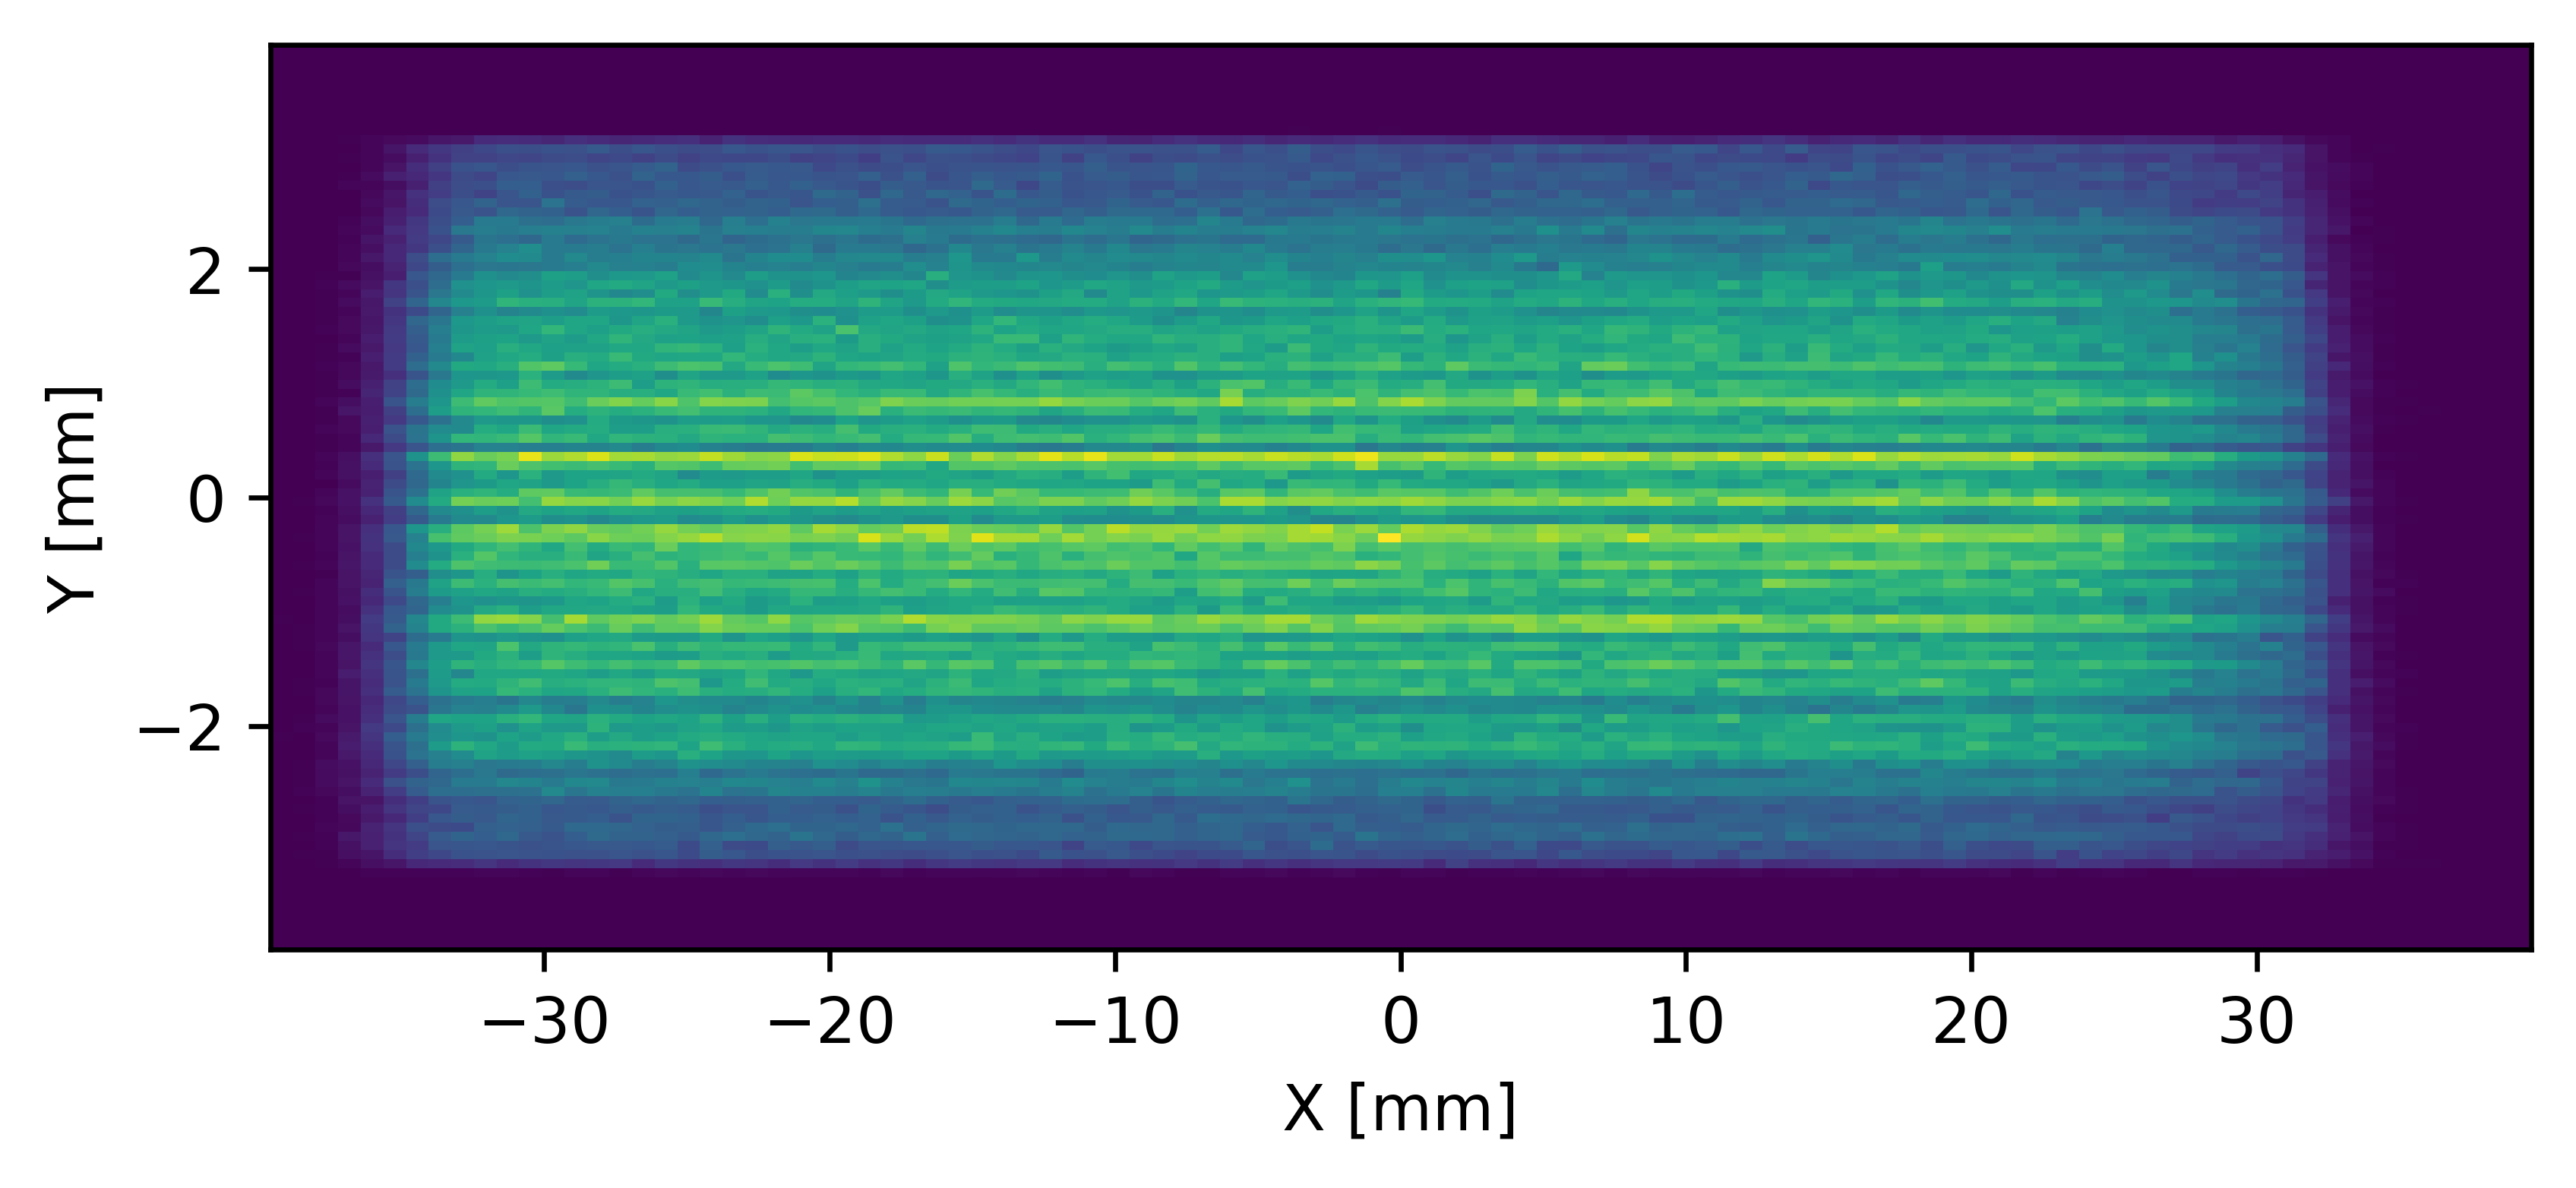
\includegraphics[width=0.9\linewidth]{./../figures/slope_error/WB4C_d30_d-spacing_gradient_45keV_slope_error02urad.png}
\end{figure}

\begin{figure}[H]
\centering
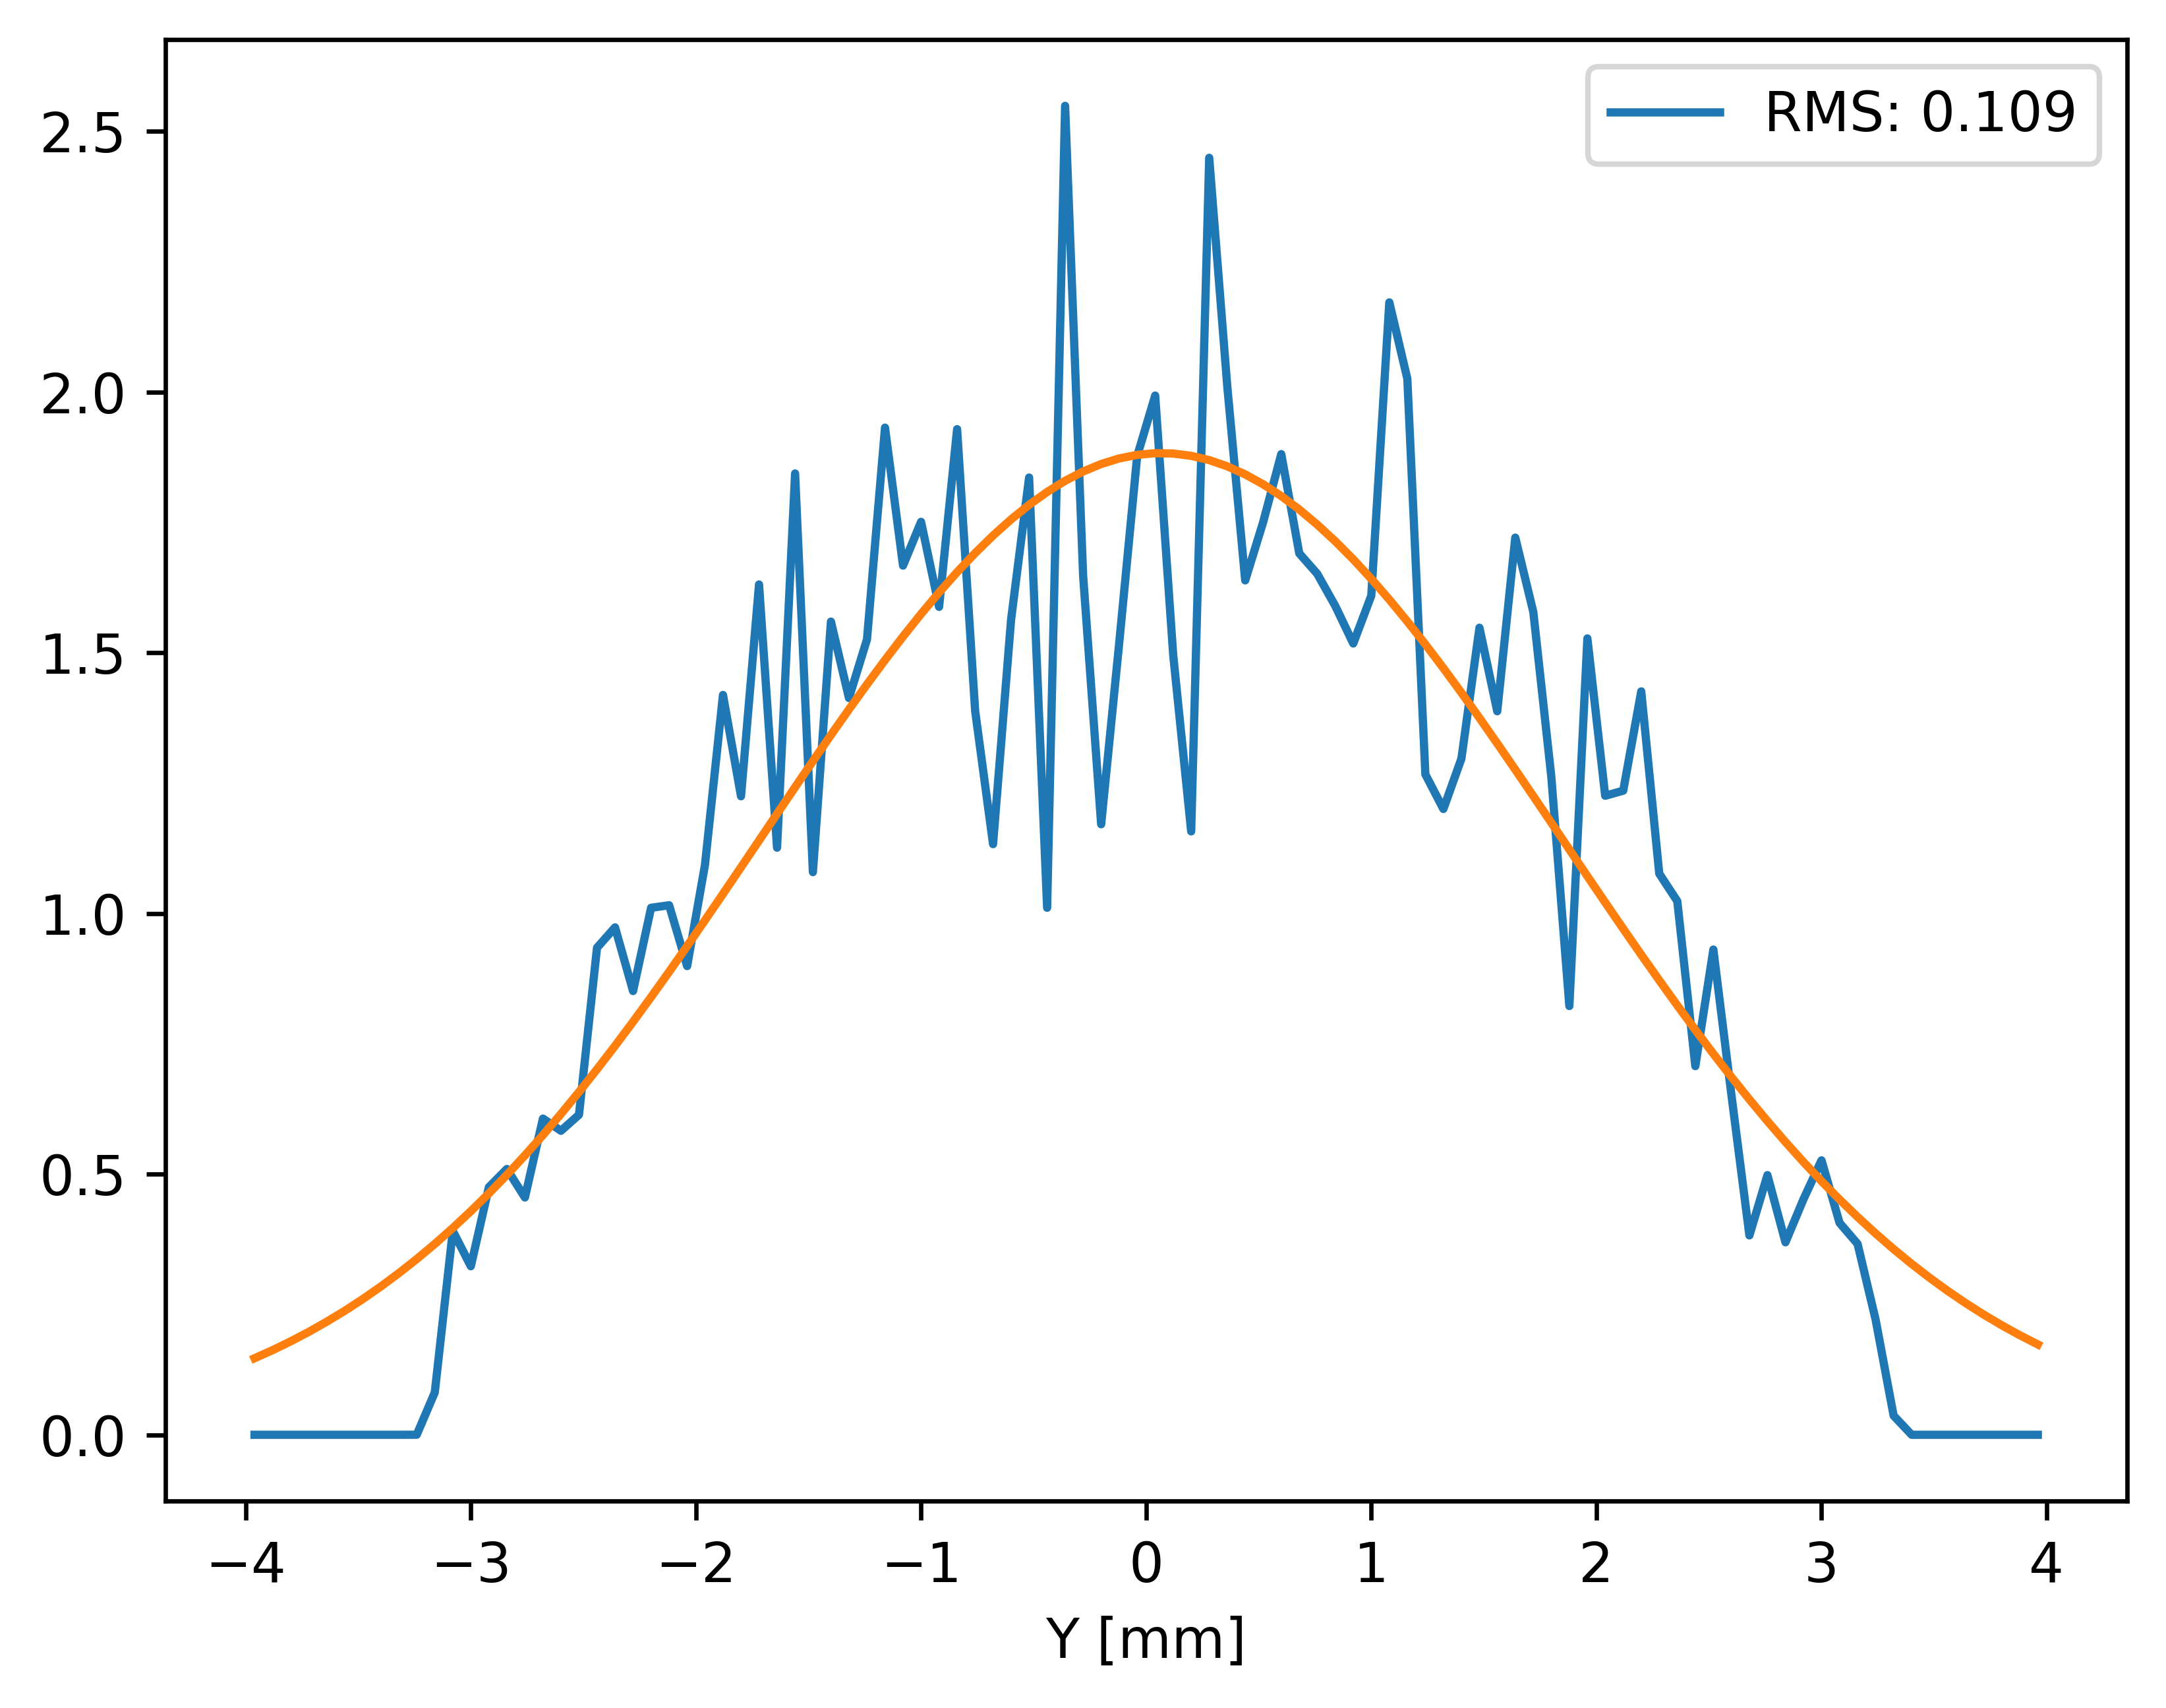
\includegraphics[width=0.9\linewidth]{./../figures/slope_error/WB4C_d30_d-spacing_gradient_45keV_slope_error02urad_ESRFID19PW150_Yprofile.png}
\caption{0.2 urad}
\label{fig:02urad}
\end{figure}

\clearpage
\subsubsection{0.3 urad}
\begin{figure}[H]
\centering
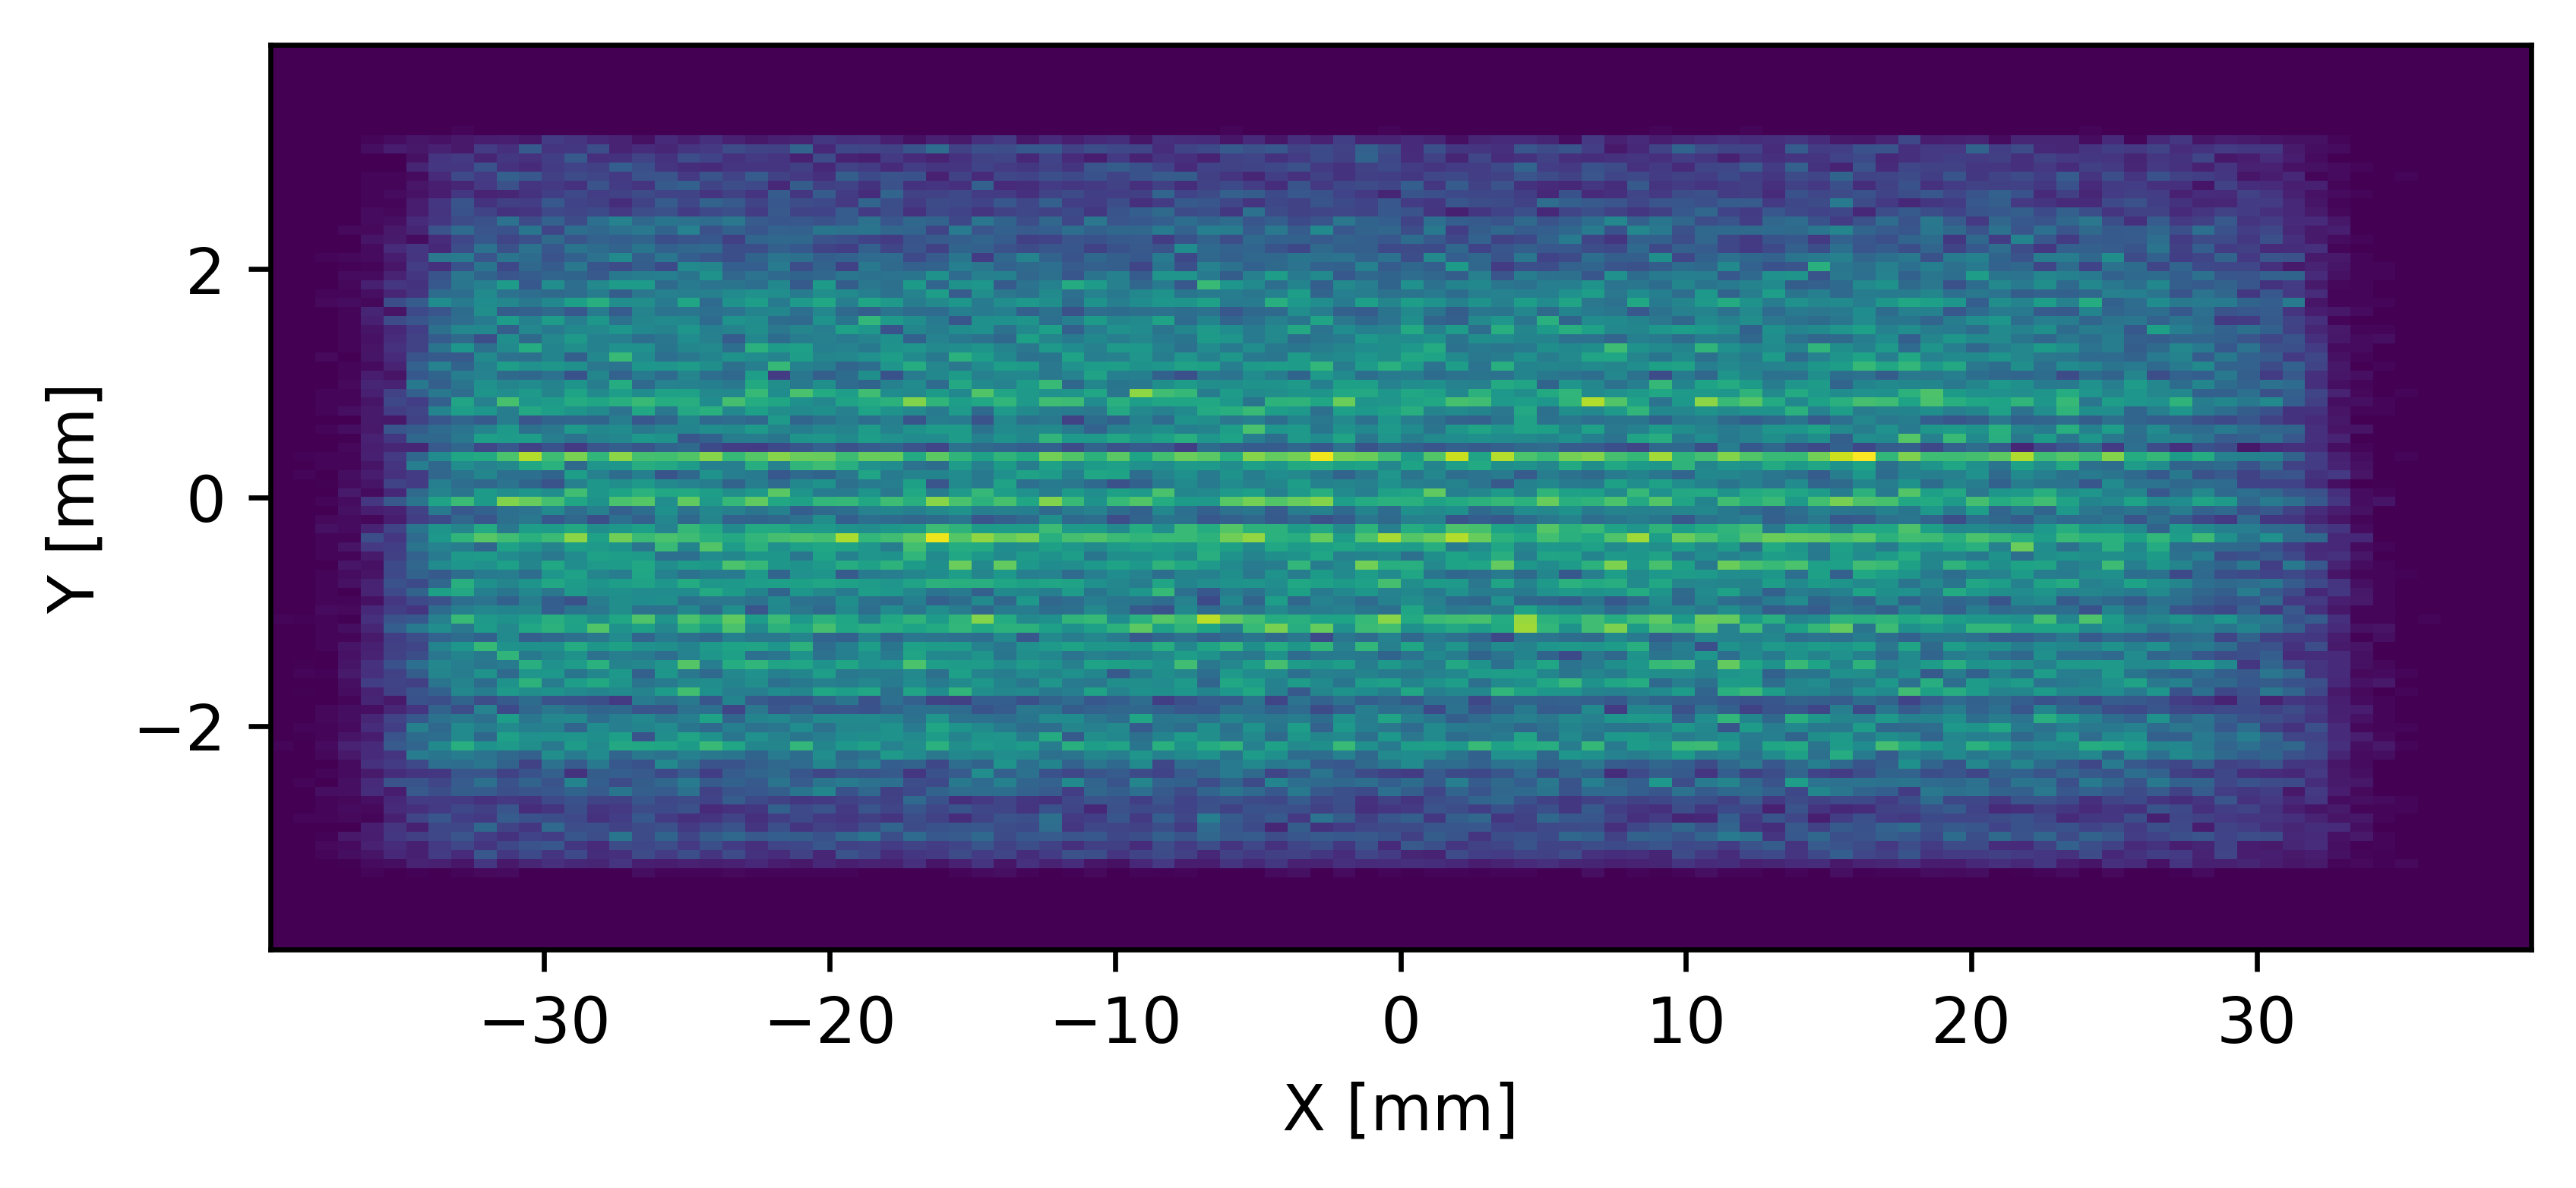
\includegraphics[width=0.9\linewidth]{./../figures/slope_error/WB4C_d30_d-spacing_gradient_45keV_slope_error03urad.png}
\end{figure}

\begin{figure}[H]
\centering
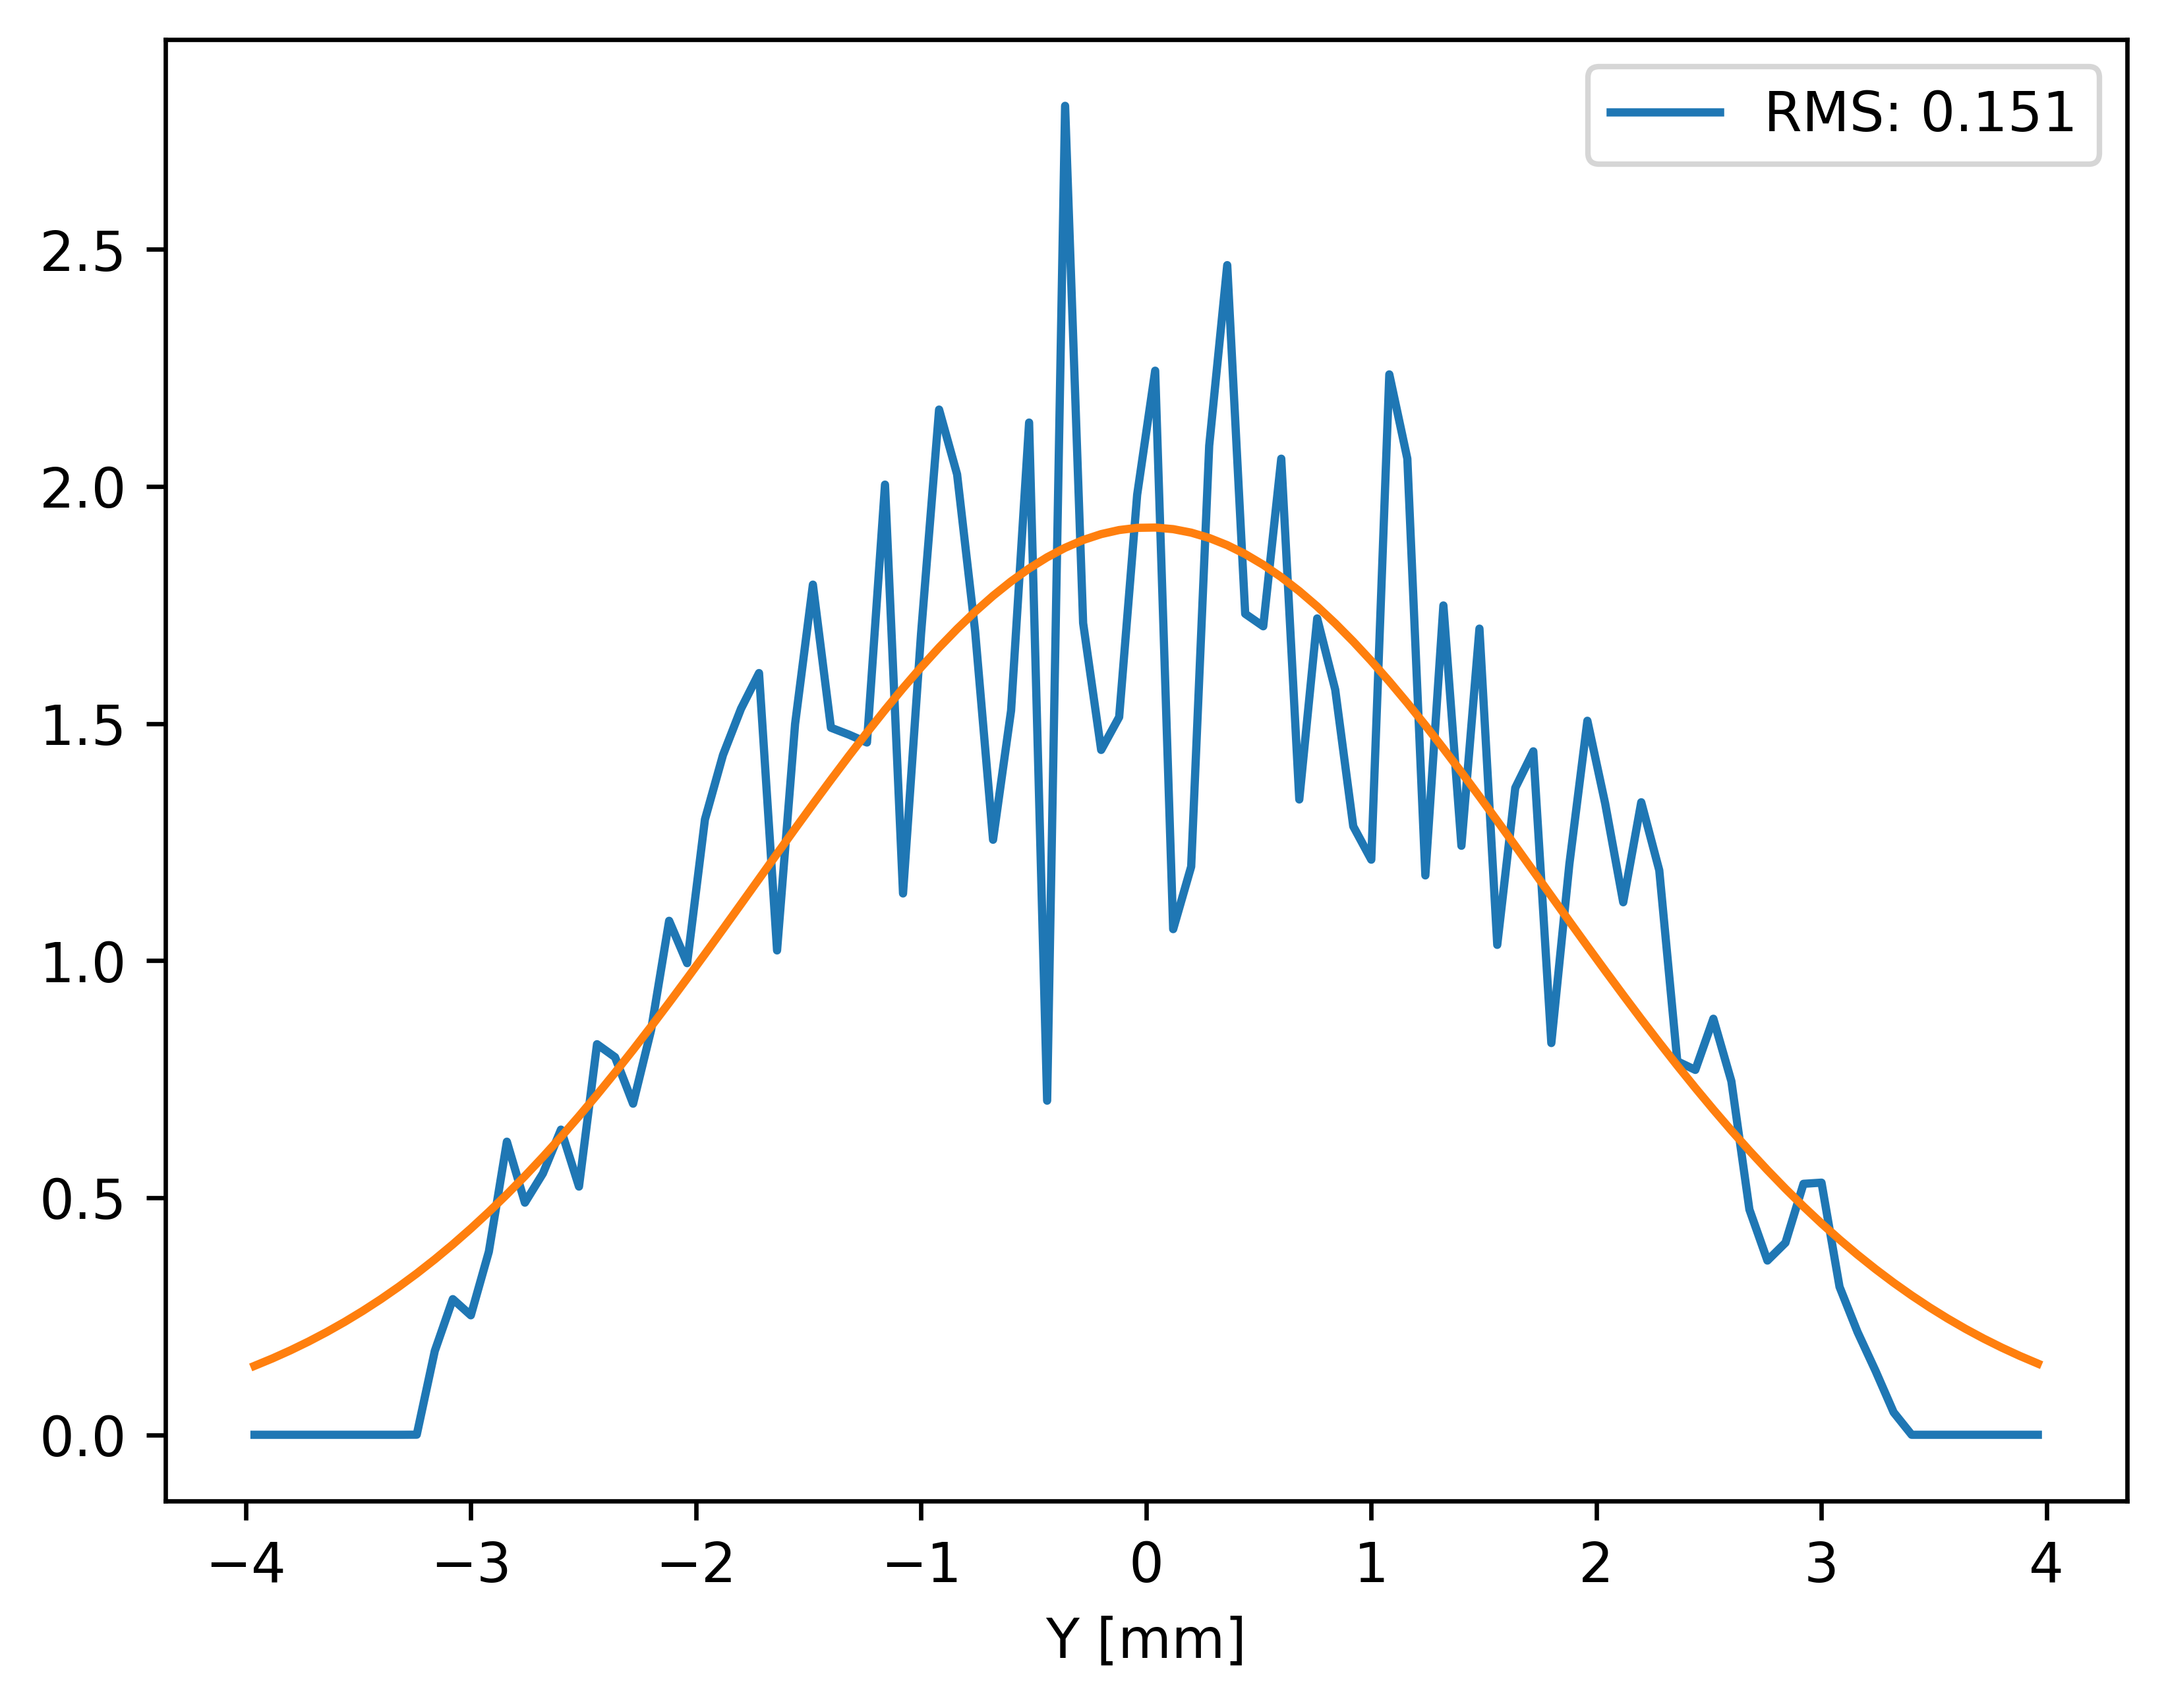
\includegraphics[width=0.9\linewidth]{./../figures/slope_error/WB4C_d30_d-spacing_gradient_45keV_slope_error03urad_ESRFID19PW150_Yprofile.png}
\caption{0.3 urad}
\label{fig:03urad}
\end{figure}

\clearpage
\subsubsection{0.4 urad}
\begin{figure}[H]
\centering
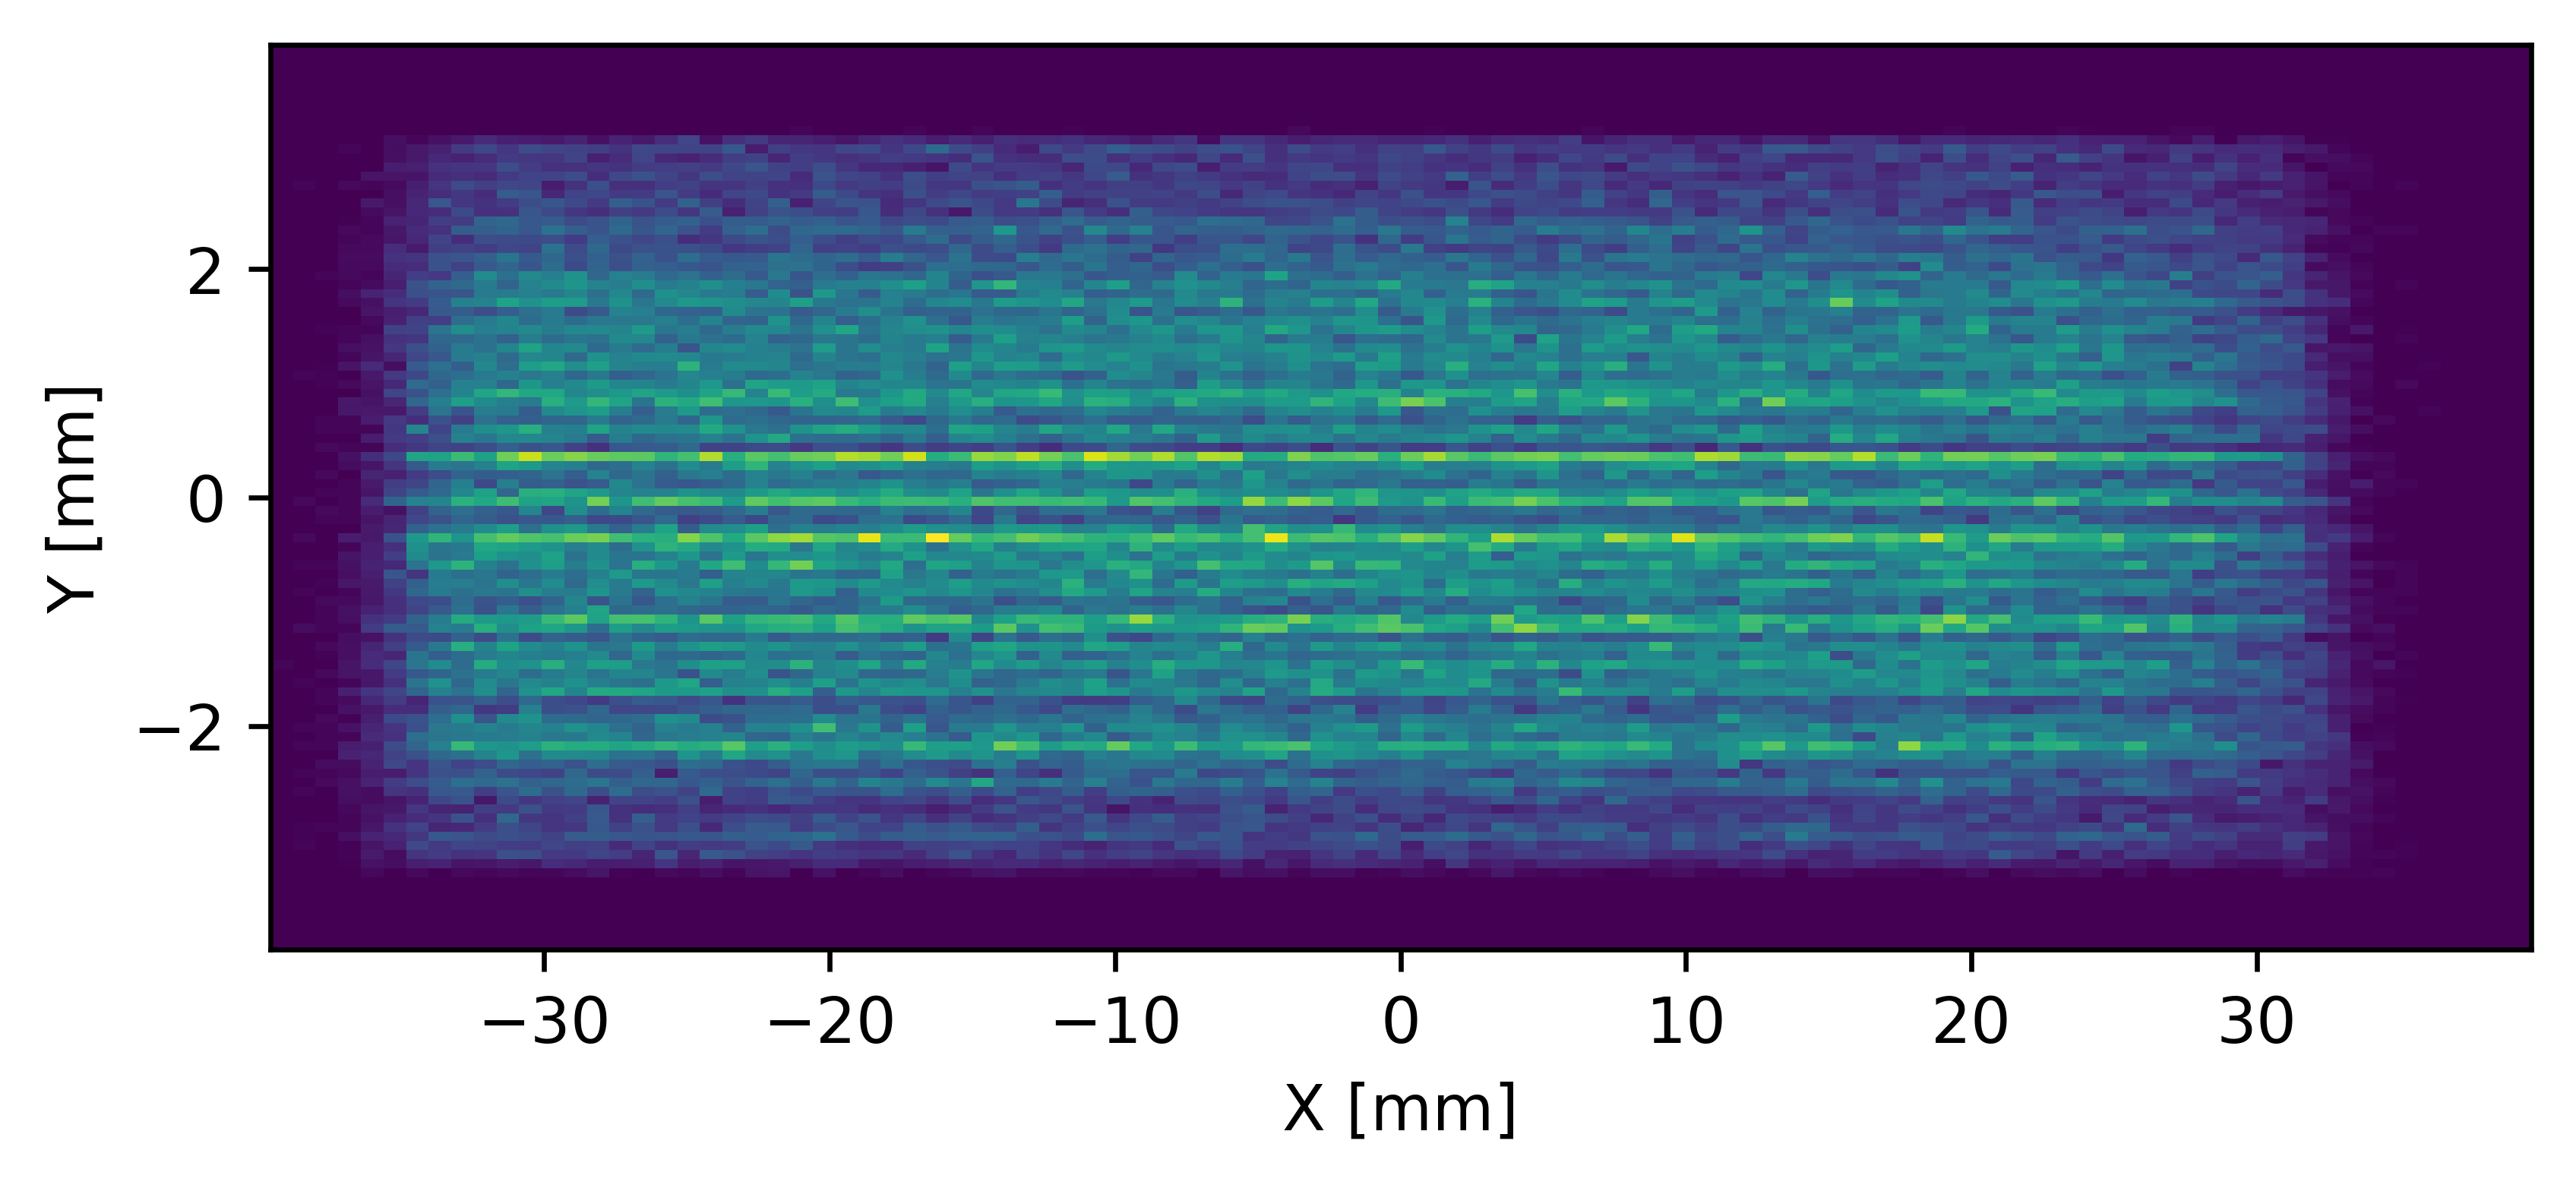
\includegraphics[width=0.9\linewidth]{./../figures/slope_error/WB4C_d30_d-spacing_gradient_45keV_slope_error04urad.png}
\end{figure}

\begin{figure}[H]
\centering
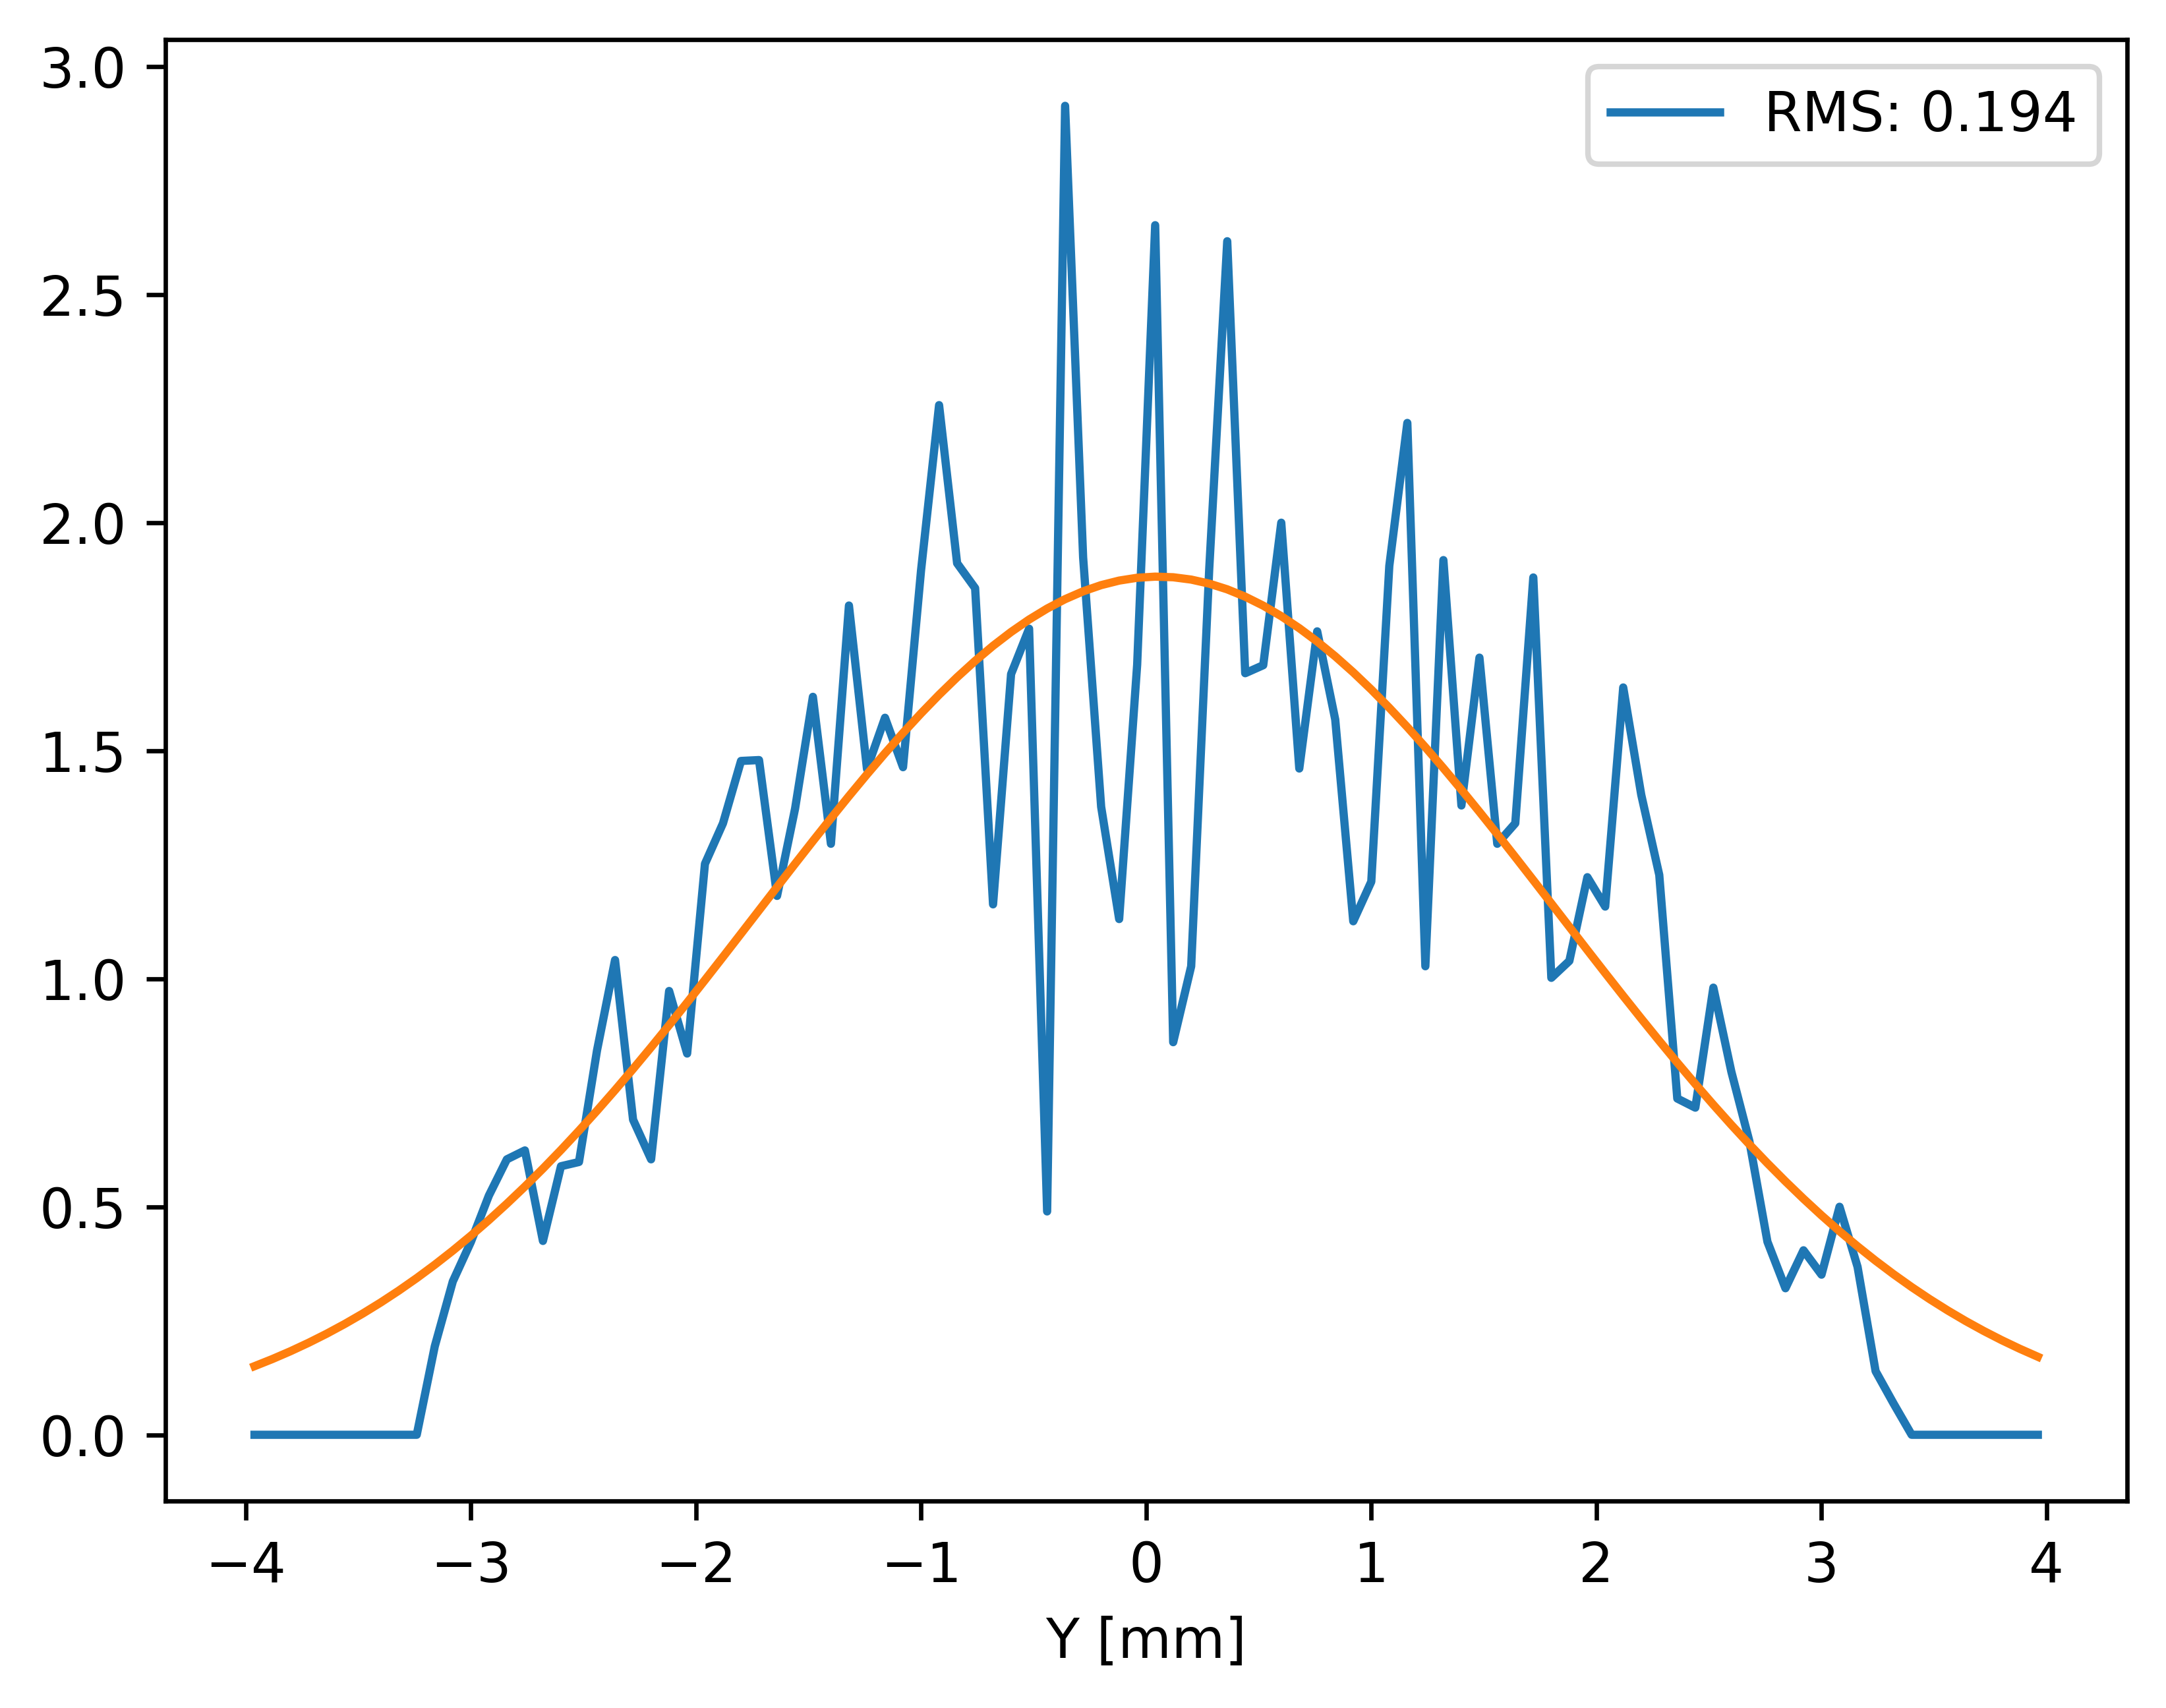
\includegraphics[width=0.9\linewidth]{./../figures/slope_error/WB4C_d30_d-spacing_gradient_45keV_slope_error04urad_ESRFID19PW150_Yprofile.png}
\caption{0.4 urad}
\label{fig:04urad}
\end{figure}

\clearpage
\subsubsection{0.5 urad}
\begin{figure}[H]
\centering
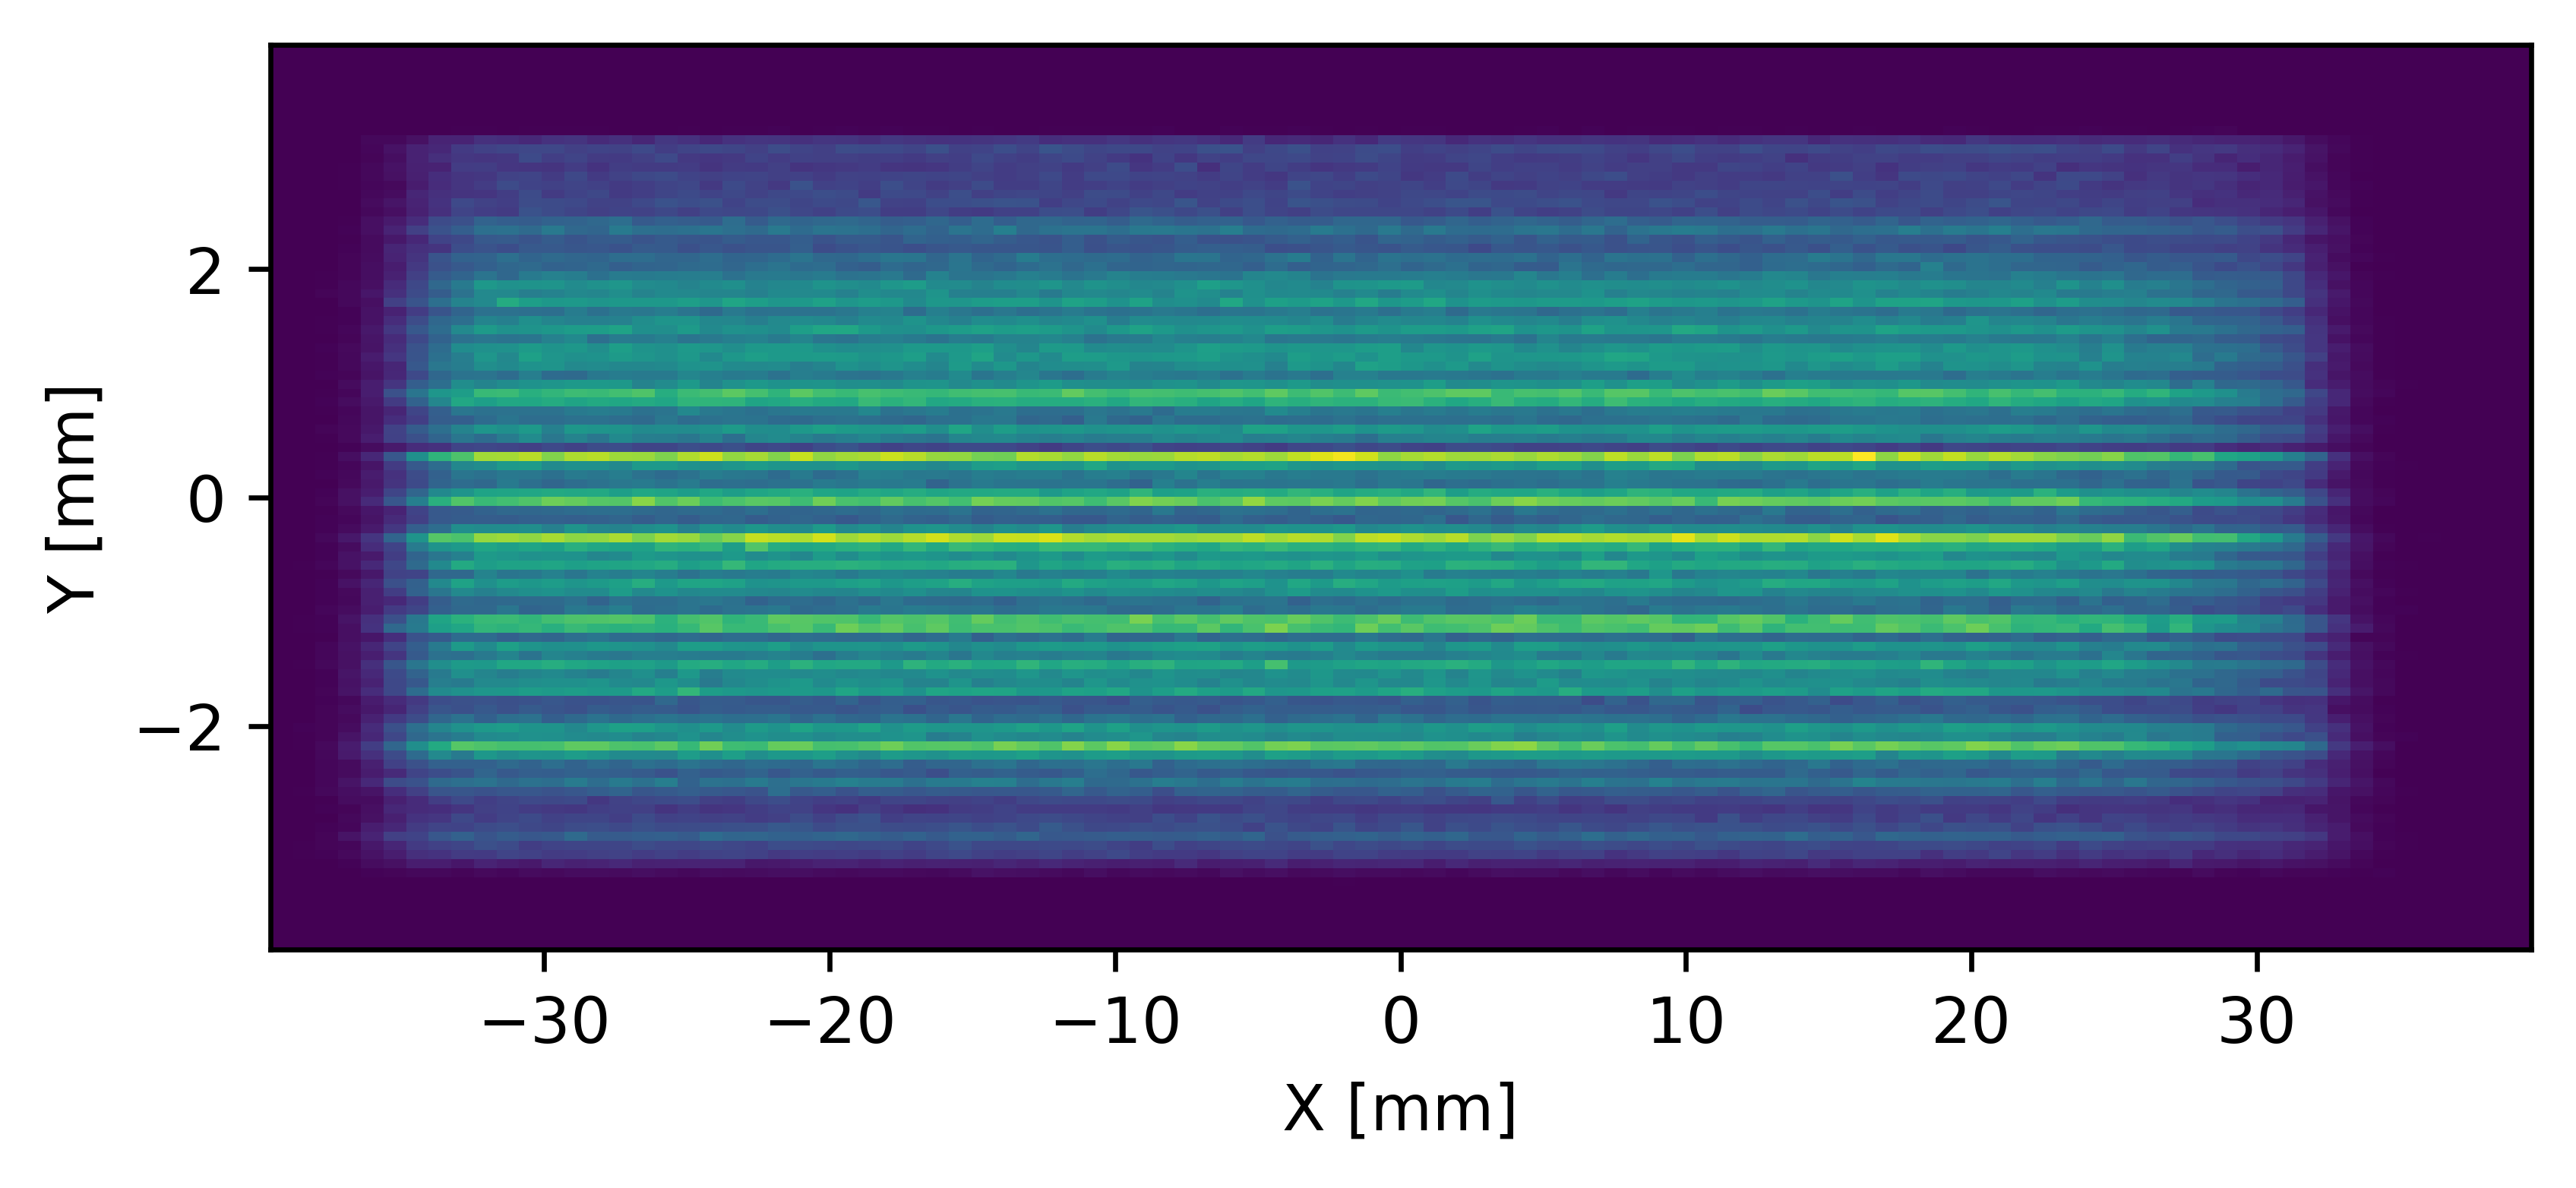
\includegraphics[width=0.9\linewidth]{./../figures/slope_error/WB4C_d30_d-spacing_gradient_45keV_slope_error05urad.png}
\end{figure}

\begin{figure}[H]
\centering
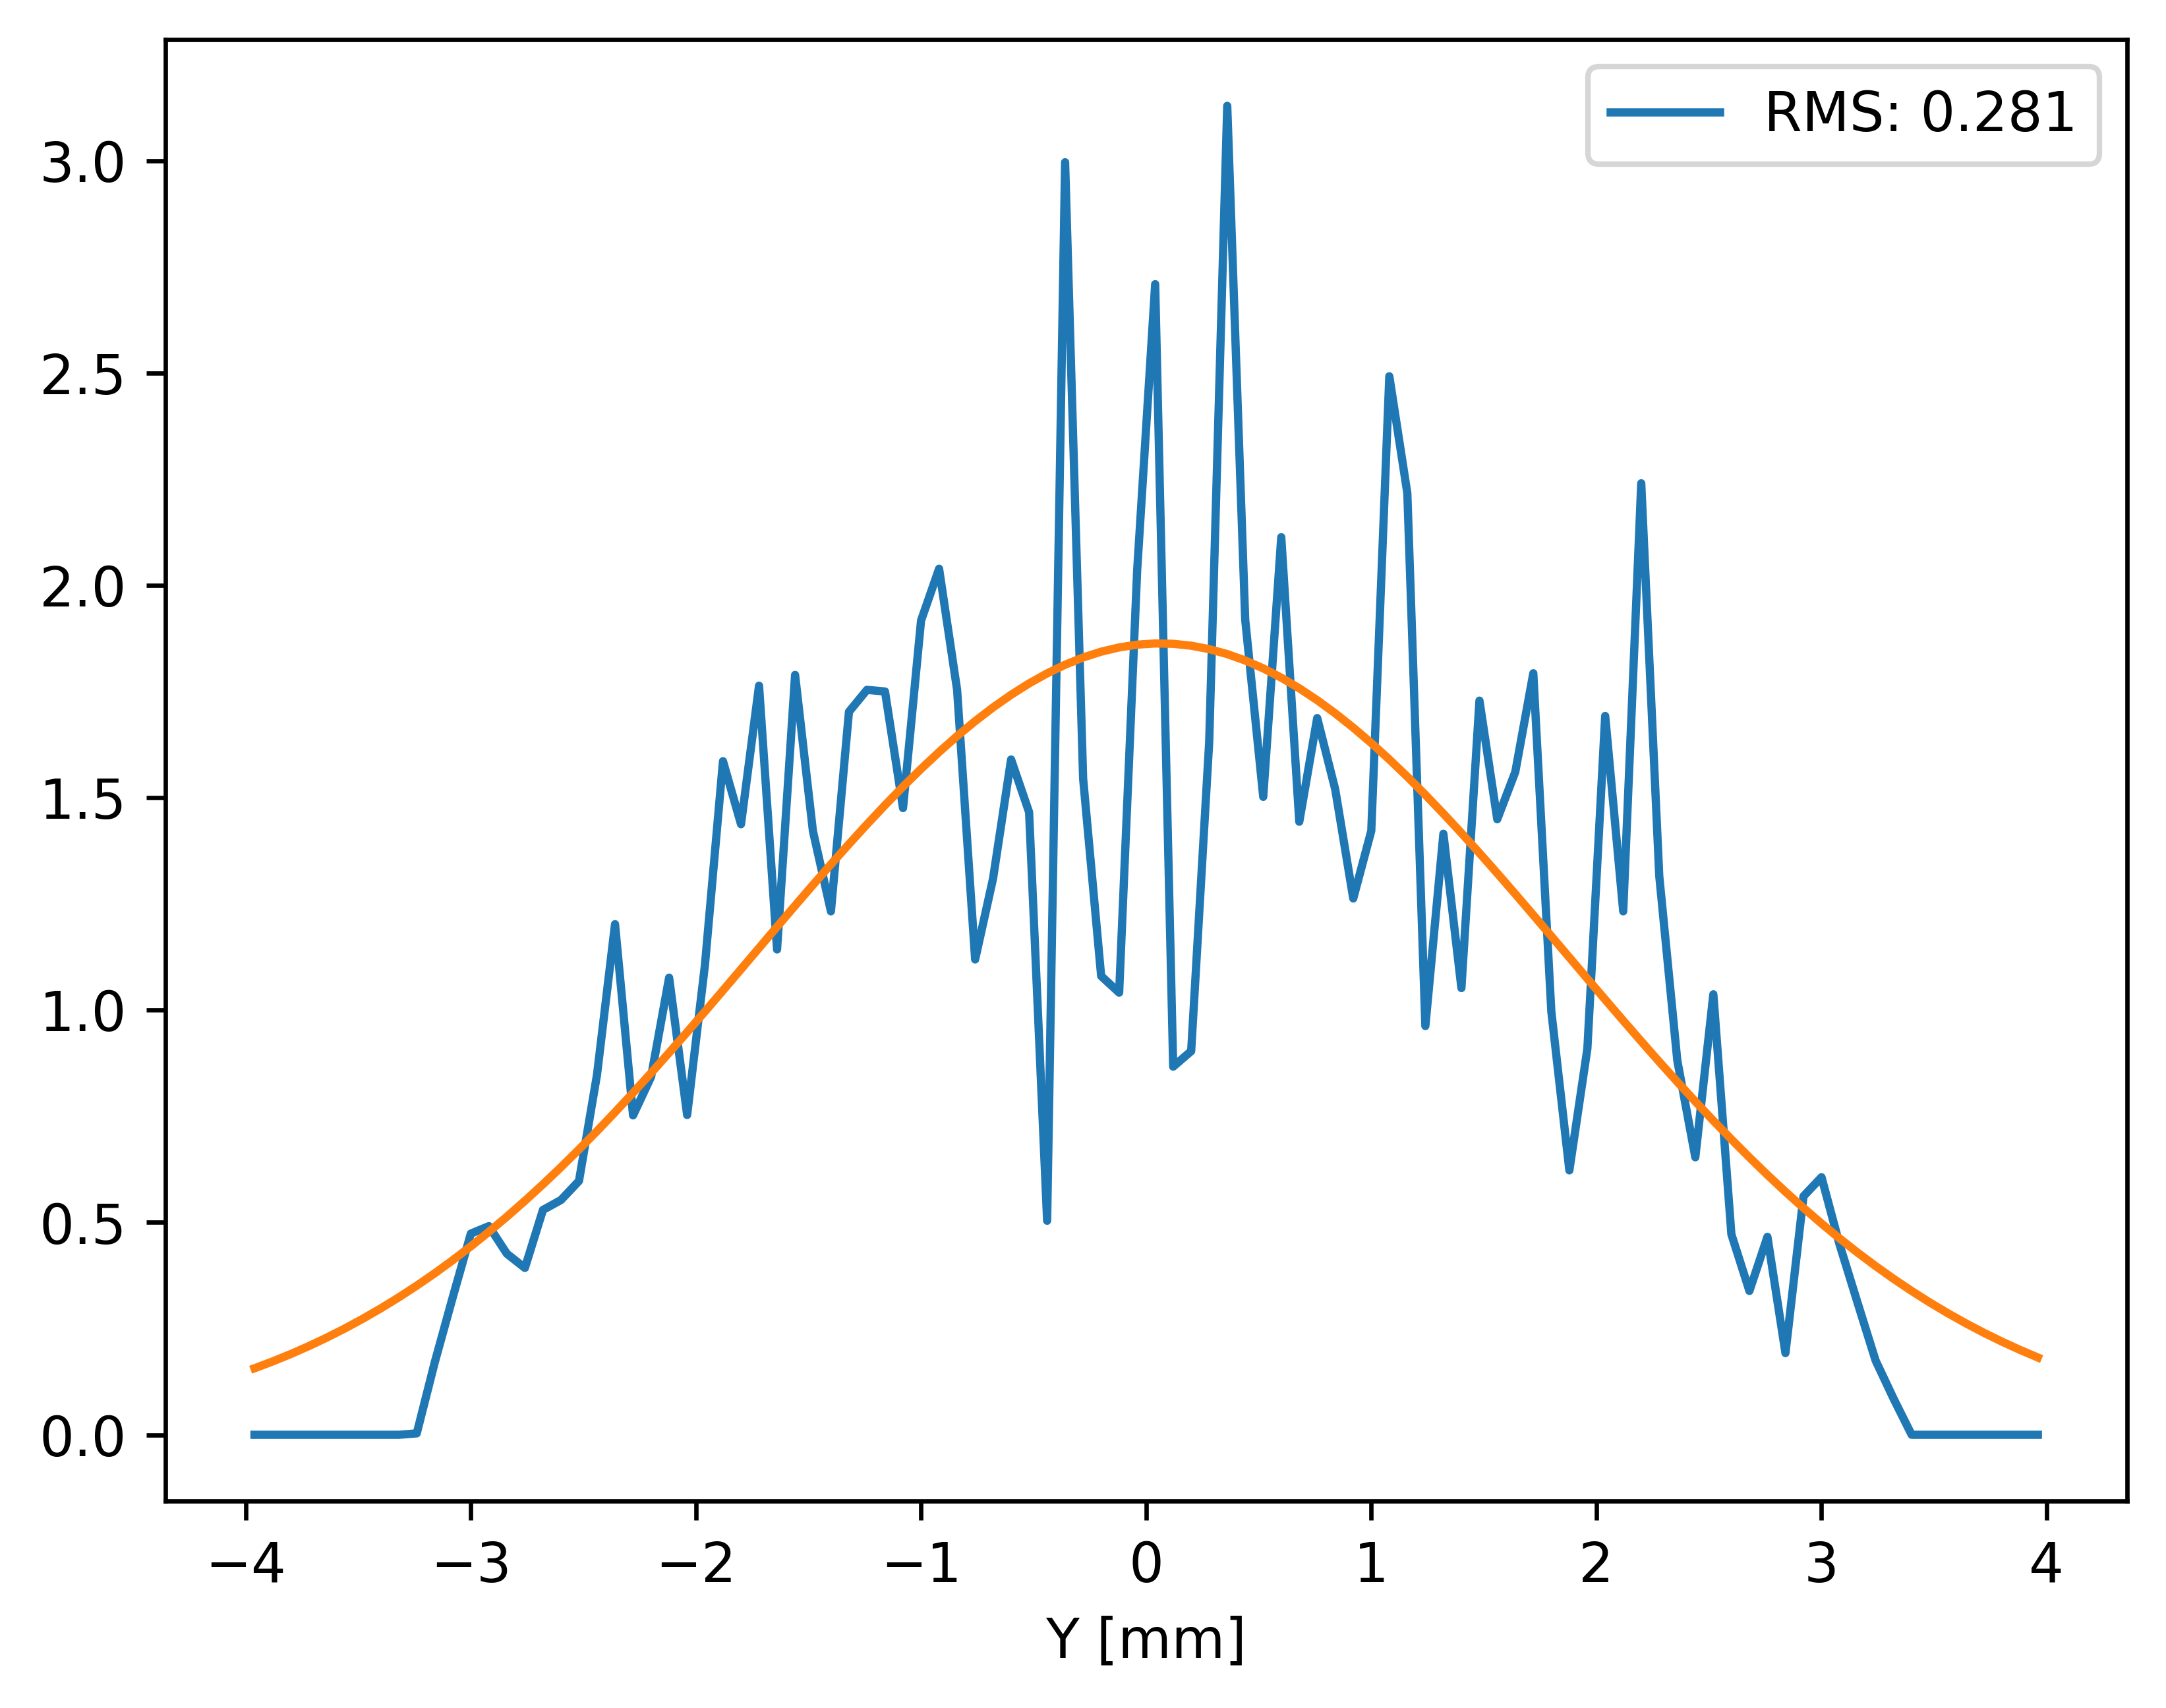
\includegraphics[width=0.9\linewidth]{./../figures/slope_error/WB4C_d30_d-spacing_gradient_45keV_slope_error05urad_ESRFID19PW150_Yprofile.png}
\caption{0.5 urad}
\label{fig:05urad}
\end{figure}


%%%%%%%%%%%%%%%%%%%%%%%%%%%%%%%%%%%%%%%%%%%%%%%%%%%%%%%%%%%%%%%%%%%%%%%%%%%%%%%%%%%%
\clearpage
\subsection{Thermal stability}
The thermal stability of ML1 should be verified with FEA simulations considering the white beam colliding with the mirror at the maximum Bragg angle allowed by the Bragg stage motorization (34.9 mrad). The thermal stability of the cooled mask in front of the ML1 profile shall be also verified.\\

The power density profile at 15.165 m from source is shown in Figure \ref{fig:power_profile_ML1}. Raw data can be found in the \powerprofilesurl. \\

\begin{figure}[ht]  % spans both columns
\begin{subfigure}{0.5\textwidth}
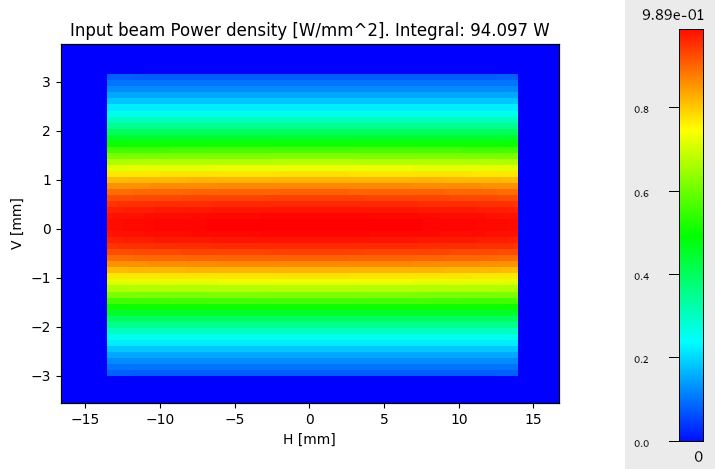
\includegraphics[width=\linewidth]{./../../power_profiles/power_profile_ML1.png}
% \caption{Network 1}
\end{subfigure}
\hfill % maximize the horizontal distance between the graphs
\begin{subfigure}{0.5\textwidth}
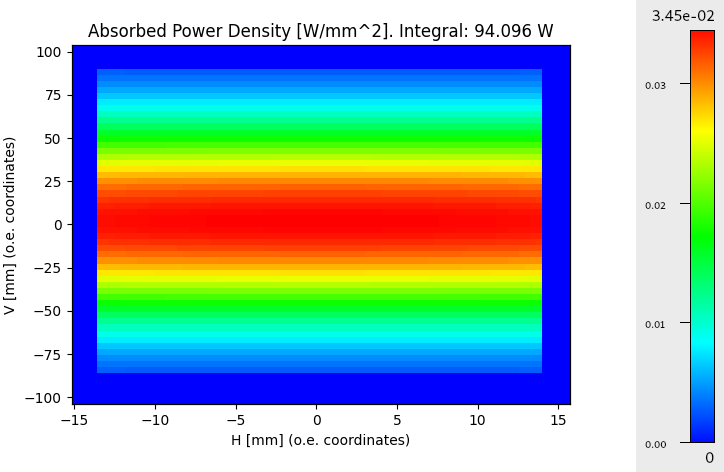
\includegraphics[width=\linewidth]{./../../power_profiles/power_profile_ML1_abs_2deg.png}
% \caption{Network  2}
\end{subfigure}
\caption{\label{fig:power_profile_ML1} Power density profile at 15.165 m from source (center position of ML1). (LEFT) Input beam. (RIGHT) Absorbed by substrate at maximum grazing (2 deg); reflectivity neglected. }
\end{figure}

